\chapter{Des atomes de Rydberg froids en environnement cryogénique}
\label{chapter:setup_coldatoms_Rydberg}
%
%INTRODUCTION DU CHAPITRE\\
%entre autres, longue vie aux Rydberg en environnement cryogénique
\vfill
\minitoc
\newpage

\noindent L'observation d'atomes de Rydberg en interaction sur des temps longs, tant pour la question du mouvement d'un gaz de Rydberg ultra-froids que dans l'optique de la simulation quantique, requiert des conditions expérimentales spécifiques.
D'une part, il est souhaitable que la durée de vie des niveaux de Rydberg soit la plus longue possible, ce qui nous pousse à travailler en environnement cryogénique.
Les calculs menés dans le chapitre \ref{chapter:Rydberg} nous montrent l'importance de la température de l'environnement sur la durée de vie des atomes de Rydberg, plus cruciale encore si l'on souhaite travailler avec des atomes de Rydberg circulaires.

D'autre part, il est nécessaire, étant donnés nos objectifs, que nos atomes de Rydberg soient aussi froids que possible.
L'on pourrait imaginer piéger et refroidir des atomes qui auraient été préalablement excités dans des niveaux de Rydberg à partir d'un jet atomique chaud.
Cependant, il n'y a pas de technique connue à ce jour qui permette cela, et la durée de vie des niveaux de Rydberg en limiterait très certainement les possibilités.
Or les techniques de piégeage et de refroidissement des atomes alcalins non excités sont des outils bien maîtrisés.
Voilà donc une piste bien plus prometteuse.

Une première difficulté se présente ici : les techniques d'atomes ultra-froids sont pour la plupart développées au sein de dispositifs à température ambiante.
Il s'agira donc ici de les concilier avec un environnement cryogénique.
Avec cette contrainte à l'esprit, et dans l'optique d'obtenir des nuages atomiques très confinés, il a été choisi de centrer le dispositif autour d'une puce à atomes supraconductrice.
Prenons note dès maintenant d'une deuxième difficulté technique posée par un tel dispositif :
les atomes de Rydberg sont extrêmement sensibles au champ électromagnétique, et nous souhaitons les exciter et les observer au voisinage de la surface conductrice qu'est notre puce atomique.

Ce chapitre sera donc dédié à la description du dispositif expérimental sur lequel nous avons effectué nos travaux.
Nous nous intéresserons d'abord à l'aspect du dispositif qui nous sert à piéger et refroidir des atomes de \Rb{87} sur une puce atomique supraconductrice.
Nous nous attacherons ensuite à décrire comment nous excitons, manipulons et détectons les atomes de Rydberg au sein de ce dispositif.

%\clearpage
\section{Un nuage d'atomes ultra-froids sur puce, du MOT de capture au condensat de Bose-Einstein}
\noindent Le développement de notre plateforme d'atomes froids autour d'une puce supraconductrice a été l'objet de plusieurs thèse de doctorat précédant celle-ci.
Les thèses de Thomas Nirrengarten \cite{PHD_NIRRENGARTEN}, de Cédric Roux \cite{PHD_ROUX} et d'Andreas Emmert \cite{PHD_EMMERT} sont dédiées à la question du piégeage et du refroidissement jusqu'au BEC d'atomes de \Rb{87} près d'une surface à l'aide de fils supraconducteurs.
La thèse de Raul Celistrino Teixeira \cite{PHD_CELISTRINO} détaille la fabrication et les caractéristiques de la puce atomique que nous avons utilisée pour nos expériences.

Nous ferons donc ici une présentation rapide du cryostat et de la puce à atomes que nous utilisons, puis nous détaillerons la suite d'étapes que nécessite le piégeage et le refroidissement des atomes de rubidium au sein de notre dispositif.
Enfin, après avoir présenté la technique d'imagerie atomique par absorption, nous présenterons quelques chiffres typiques de nos nuages atomiques.


\subsection{L'environnement cryogénique : cryostat et puce à atomes supraconductrice}\label{subsec:cryopuce}
\noindent L'environnement cryogénique présente un avantage incomparable pour la durée de vie des atomes de Rydberg, mais impose aussi quelques spécificités à notre dispositif d'atomes froids.
Le piégeage d'atomes froids pendant des durées suffisantes à leur manipulation exige un vide très poussé dans l'enceinte expérimentale, car les collisions avec les molécules de gaz résiduel éjectent les atomes hors de leur piège.
Les chambres de piégeage d'atomes neutres à température ambiante sont généralement étuvées pendant plusieurs semaines afin d'atteindre des pressions de gaz résiduel suffisamment faibles.
Dans un environnement cryogénique au contraire, les parois froides de l'enceinte adsorbent une grande partie du gaz résiduel, et des pressions très inférieures à \SIvv{1e-10}{\milli\bar} sont obtenues sans étuvage.
Travailler en environnement cryogénique permet en outre l'utilisation de fils et de bobines supraconducteurs pour le passage des courants électriques qui génèrent les champs magnétiques nécessaires au piégeage des atomes.
Des courants de quelques Ampères sont ainsi passés sans dissipation et à proximité des atomes piégés, alors qu'une expérience d'atomes froids à température ambiante nécessite des bobines qui soient placées en-dehors de la chambre et refroidies par des circuits d'eau dédiés.

L'environnement cryogénique pour les atomes froids a cependant quelques inconvénients :
en premier lieu, l'accès optique est limité car les parois de l'enceinte doivent être opaques pour le rayonnement du corps noir et donc métalliques, chaque hublot de verre réduisant l'isolation thermique du c\oe ur de l'expérience.
En second lieu, l'utilisation d'hélium et d'azote liquide à proximité d'un vide poussé présente une lourdeur technique supplémentaire au quotidien.

\subsubsection*{Le cryostat}
\noindent Notre expérience est placée au c\oe ur du cryostat représenté en figure \eqref{fig:cryo}.
%
\begin{figure}
\centering
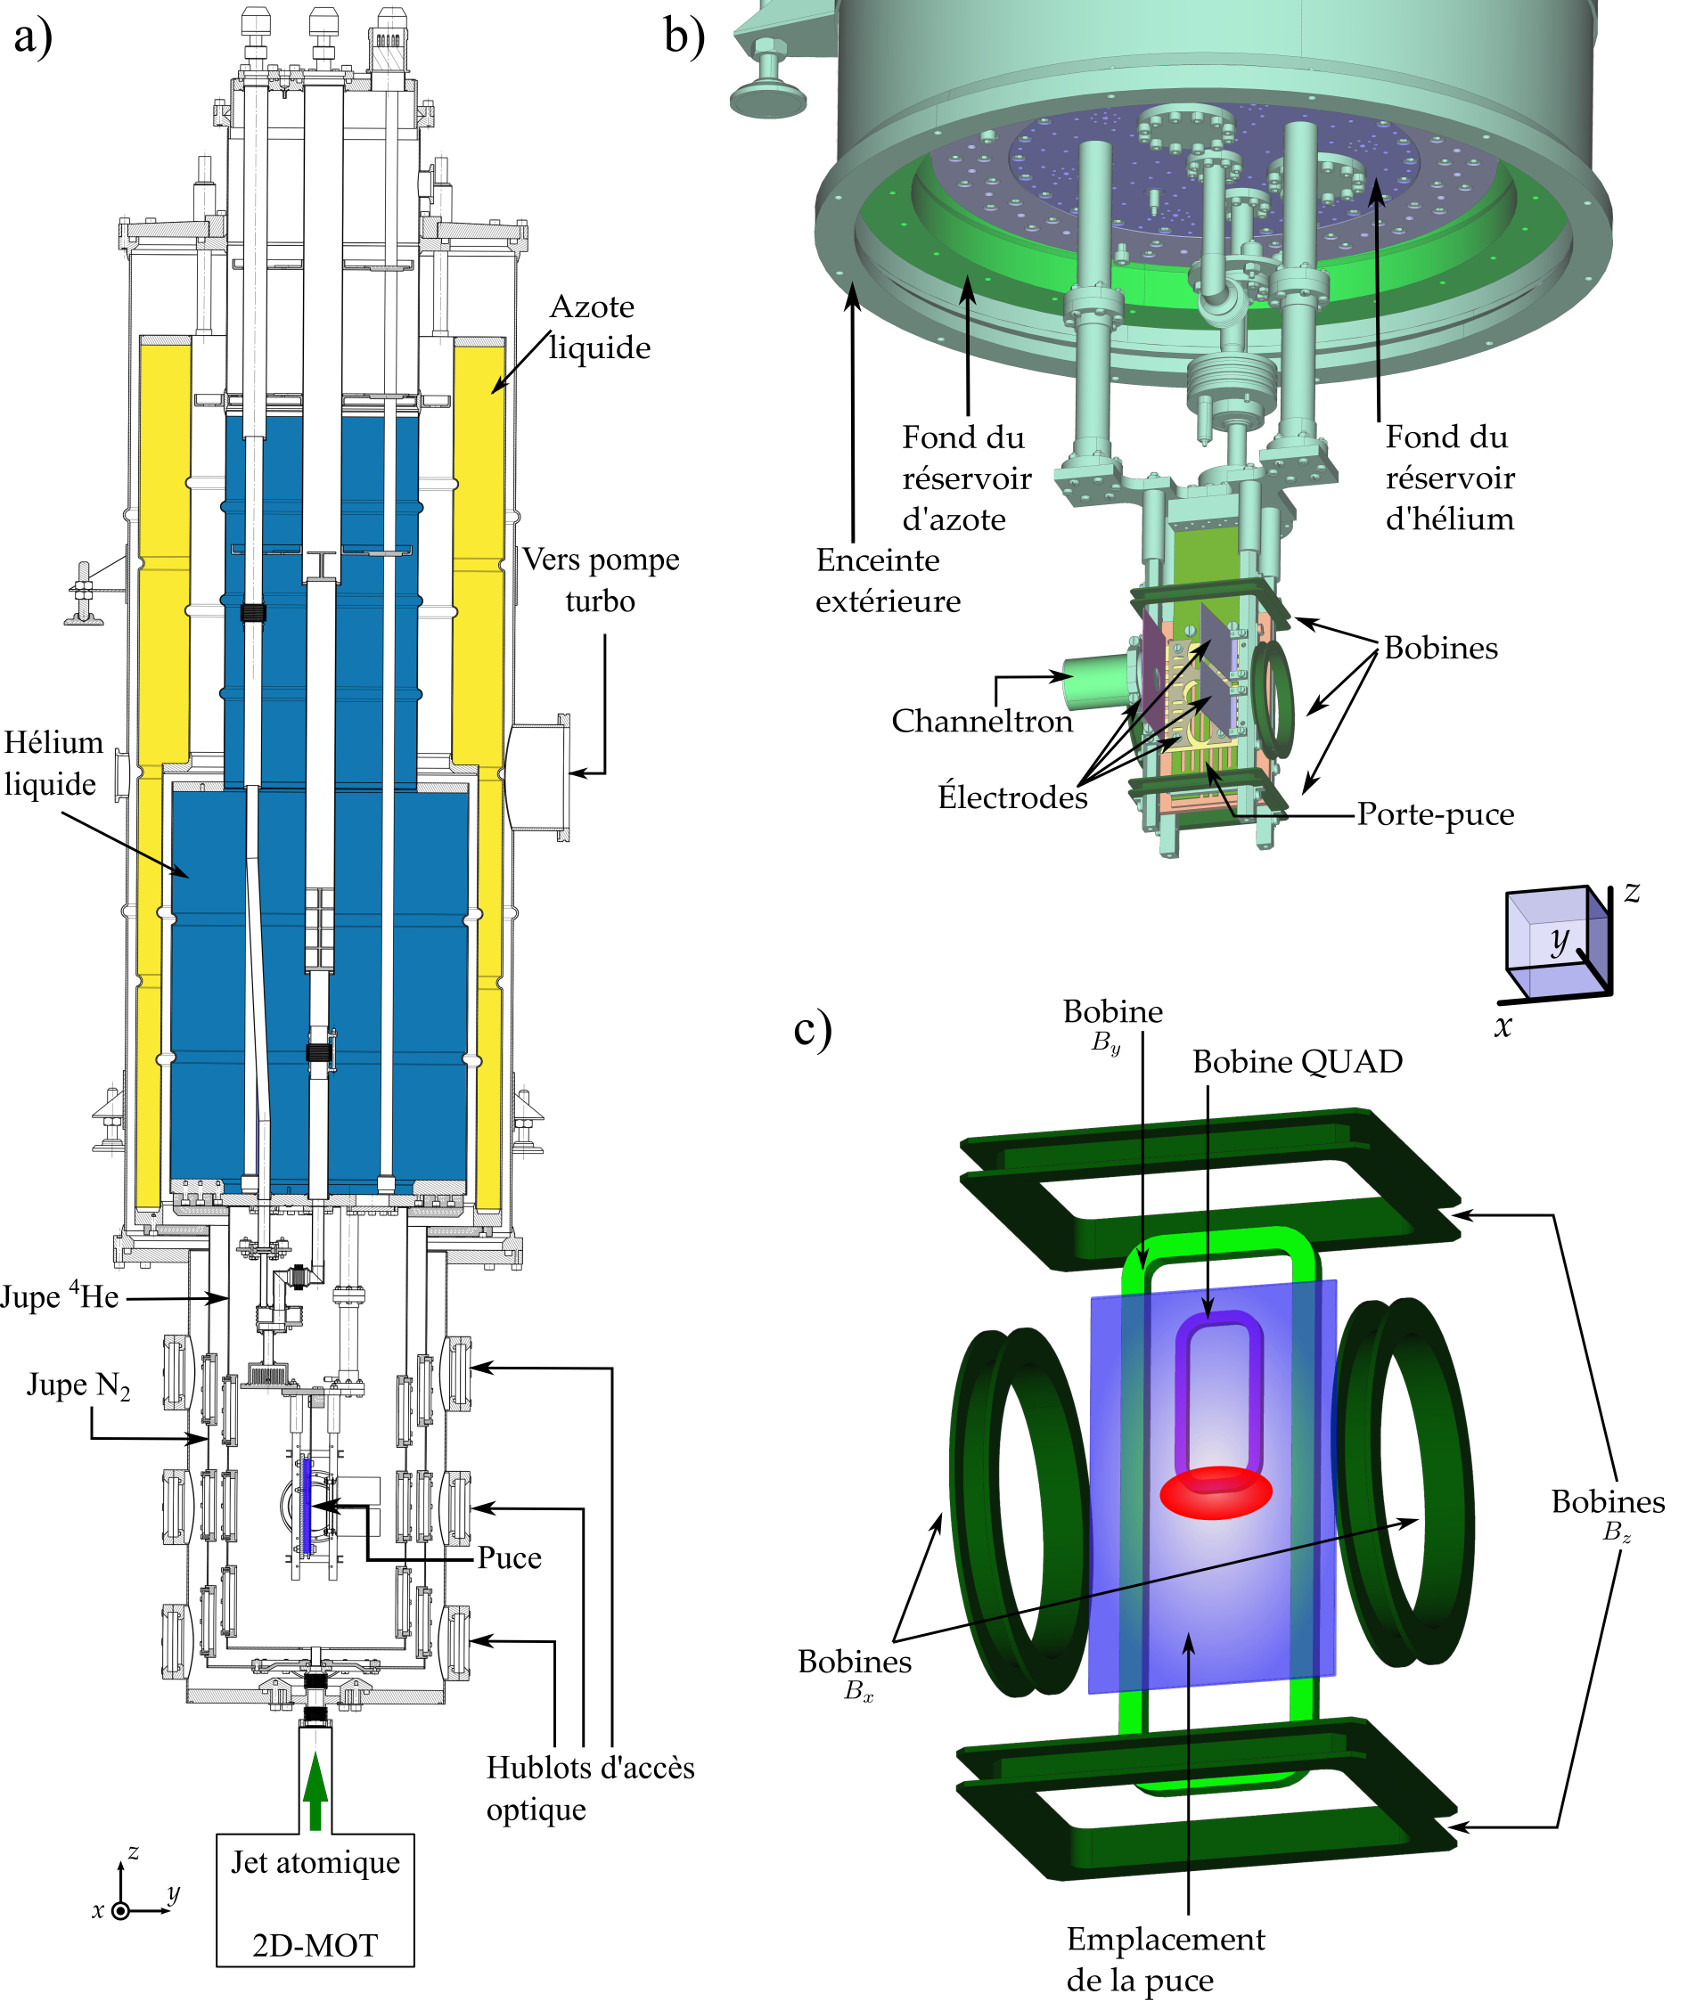
\includegraphics[width=\linewidth]{figures/setup/coldatoms/cryo_vect2.jpg}
\caption[Schéma du cryostat]{Schéma du dispositif cryogénique :
\textbf{a)} Coupe du du cryostat, avec la puce (colorée en violet) tournée vers le côté droit.
Le réservoir d'azote liquide est indiqué en jaune, le réservoir d'hélium liquide en bleu.
Le c\oe ur de l'expérience est visible, ainsi que les deux \og jupes \fg{} et l'enceinte extérieure à température ambiante.
Cinq hublots, trois en face de la puce et un sur chaque côté, sont installés sur chacune de ces jupes pour l'accès optiques.
Derrière la puce, du côté gauche du schéma, les hublots optiques sont remplacés par des disques métalliques.
Les atomes proviennent du \og 2D-MOT \fg{}, une enceinte externe située sous le cryostat, où l'on réalise un piège magnéto-optique à deux dimensions.
\textbf{b)} Vue schématique du c\oe ur de l'expérience. La puce est fixée sur le porte-puce et fait face à la direction $y$. Les bobines (vert foncé) servent à créer des champs magnétiques pour le piégeage des atomes de rubidium.
Le channeltron et les différentes électrodes représentées servent à la détection des atomes de Rydberg. On ne voit pas les \og jupes \fg{} d'azote et d'hélium, ni l'enceinte extérieure.
\textbf{c)} Vue de près des bobines : la bobine QUAD (mauve) génère un champ quadrupolaire pour faire un MOT sur puce. L'emplacement de la puce est représenté par le rectangle bleu devant la bobine QUAD et la bobine $B_y$ (vert clair).
La zone rouge indique l'endroit où les atomes de rubidium sont piégés, devant la puce.
Les axes sont les mêmes qu'en \textbf{b)}.
}
\label{fig:cryo}
\end{figure}
%
La conception de ce cryostat a été évoquée dans la thèse de Raul Celistrino Teixeira \cite{PHD_CELISTRINO}  et discutée plus en détail dans les thèses de Thomas Nirrengarten \cite{PHD_NIRRENGARTEN} et Cédric Roux \cite{PHD_ROUX}.
Le c\oe ur de l'expérience est protégé de la radiation extérieure par des écrans thermiques (\og jupes \fg{}) en cuivre doré. Ce sont des cylindres ouverts en haut et vissés sur le fond des réservoirs de liquides cryogéniques.
La jupe $^4 \text{He}$ est vissée sur le fond du réservoir d'hélium 4 et la jupe $\text{N}_2$ est vissée au fond du réservoir d'azote liquide.
Elles sont donc respectivement thermalisées à \SIvv{4.2}{\K} et \SIvv{77}{\K}.
Sur chaque jupe, cinq hublots sont installés pour l'accès optique à la zone de piégeage :
deux sur les directions $\pm x$, un dans la direction $+y$ qui fait face à la puce, et deux  dans le plan $yz$, de part et d'autre du hublot de face sur les bissectrices des axes $+y$ et $\pm z$, appelées direction $\pm\SIvv{45}{\degree}$ respectivement.
Par ces hublots, tous les faisceaux laser atteignent la zone de piégeage au c\oe ur de l'expérience.
Tous les éléments qui sont installés à l'intérieur de la jupe hélium sont thermalisés à \SIvv{4.2}{K} par contact thermique avec le réservoir d'hélium liquide.

L'intérieur de la jupe hélium est revêtu d'une couche de plomb, supraconducteur à \Khe. Cette couche de plomb écrante les champs magnétiques extérieurs par effet Meissner \cite{MX_MEISSNEREFFECT}, et évite les courants de Foucault qui se créeraient dans les jupes en cuivre à l'allumage ou à l'extinction des courants dans les bobines. 
Il reste nécessaire cependant d'imposer un champ extérieur de compensation au moment du refroidissement, afin que la couche de plomb ne piège pas de lignes de champ magnétique provenant de l'environnement.
Cette compensation du champ constant de l'environnement est réalisée à l'aide de grandes bobines placées à l'extérieur du crysotat.

Enfin, bien que les jupes ne soient pas parfaitement étanches, elles garantissent un vide différentiel entre la partie du cryostat à \SIvv{300}{\K}, où la pression vaut \SIvv{1.5e-7}{\milli\bar}, et la partie à \Khe, où la pression est inférieure à \SIvv{1e-10}{\milli\bar}\footnote{
Cette valeur n'est pas mesurée en raison de l'absence de sonde de pression dans cette région du cryostat, mais inférée à partir du temps de vie des nuages d'atomes piégés, qui est de l'ordre de la minute \cite{ENS_CHIPLIFETIME}.}.

%\clearpage
\subsubsection*{La puce à atomes}
\noindent La puce à atome qui siège au c\oe ur de notre expérience est représentée en figure \eqref{fig:chip}.
C'est une puce assez simple, conçue autour de trois fils supraconducteurs : le fil (LJ), en forme de \mcal{U}, le fil (LG) en forme de \mcal{Z}, et le fil (KM) droit.
Ces fils sont fabriqués par dépôt de niobium d'une épaisseur de \SIvv{2}{\um} sur un substrat de silicium recouvert d'une couche d'oxyde SiO$_2$.
Le dépôt de niobium est ensuite gravé, et l'ensemble de la puce est recouvert d'une couche d'or de \SIvv{200}{\nm} d'épaisseur afin de rendre la surface réfléchissante.
Le niobium étant supraconducteur à $\SI{4.2}{\K}$, les courants électrique pourront toujours passer par les fils de la puce et non par la couche d'or qui reste dans un de état conducteur normal.
Les détails de la fabrication de la puce sont présentés en annexe dans la thèse de Raul Celistrino Teixeira \cite{PHD_CELISTRINO}.
%
\begin{figure}[!h]
\centering
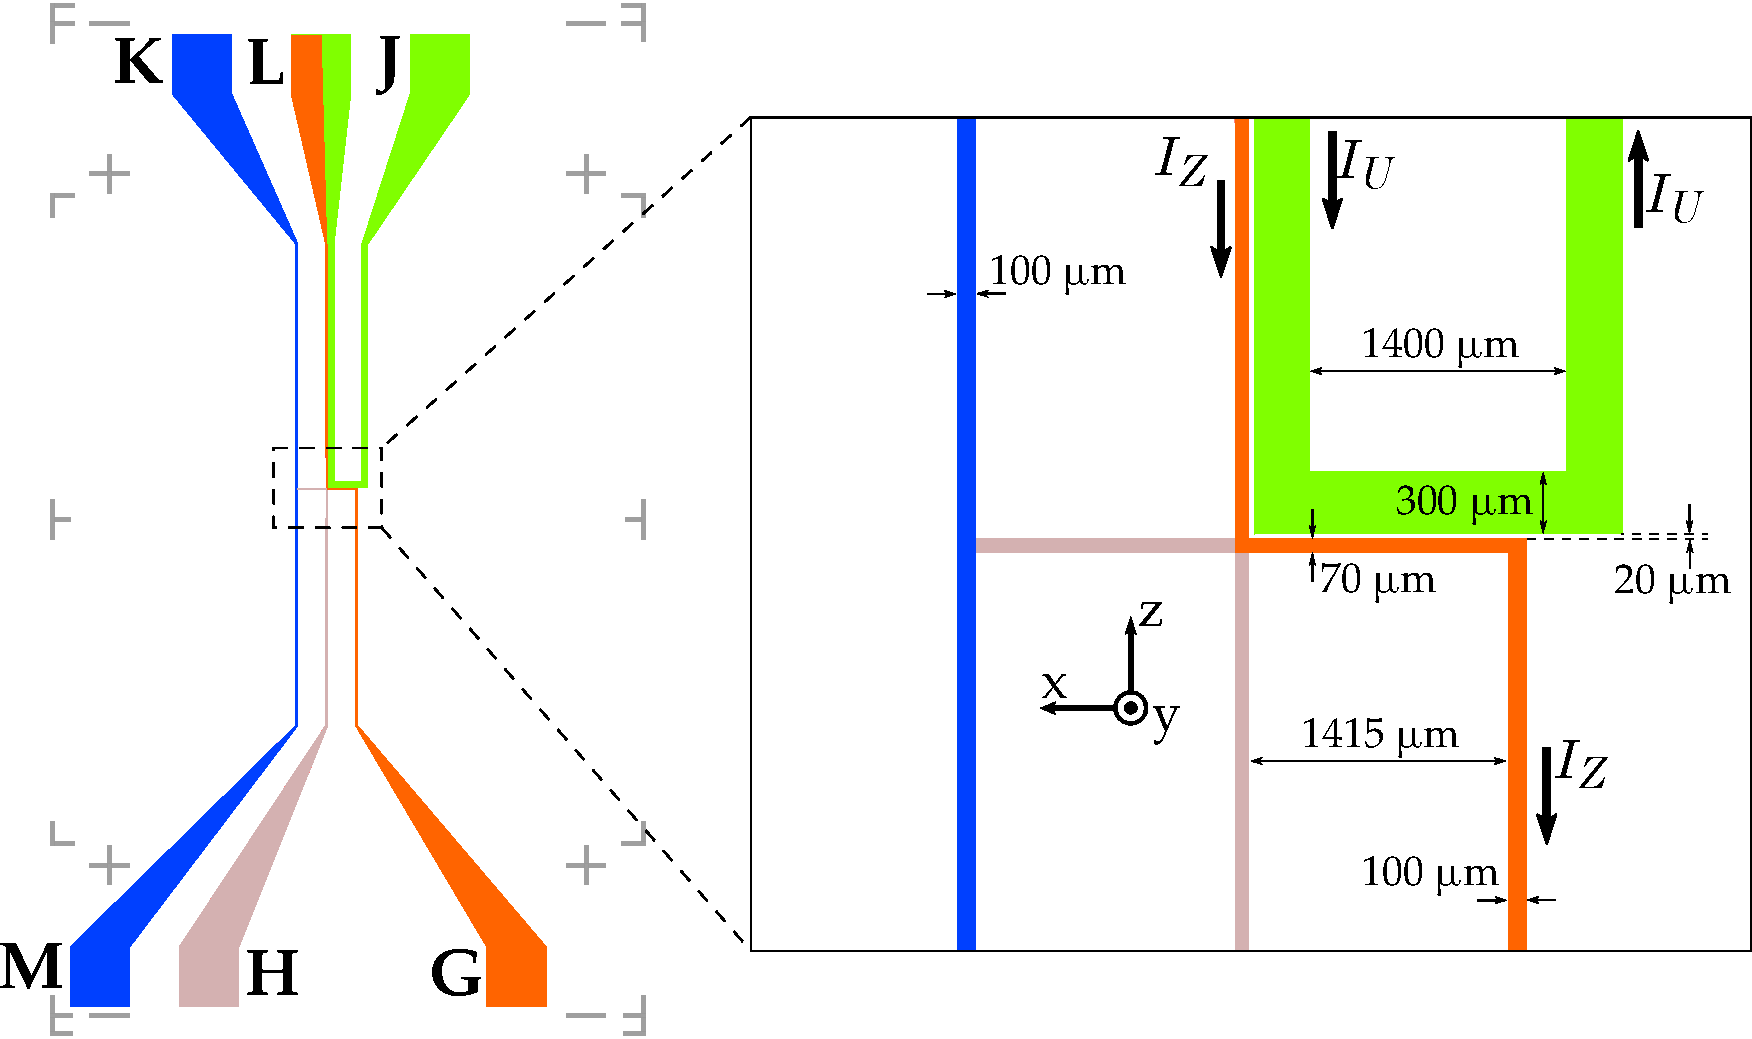
\includegraphics[width=\linewidth]{figures/setup/coldatoms/chip}
\caption[Schéma de la puce à atomes supraconductrice]{Schéma de la puce supraconductrice.
Les lettres étiquettent les pattes d'entrée/sortie des courants électriques sur la puce.
Les couleurs sont une aide visuelle pour mieux suivre les fils : en vert, le \og fil \mcal{U}\fg{}, en orange le \og fil \mcal{Z}\fg{} et en bleu le \og fil RF \fg{}.
\`A droite, vue de près du centre de la puce, qui détaille la largeur des fils, la distance entre eux et le sens de circulation des courants.
Les axes $x,y$ et $z$ coïncident avec ceux de la figure \eqref{fig:cryo}.
}
\label{fig:chip}
\end{figure}
%

Les fils en \mcal{U} et en \mcal{Z} sont la simplification d'un dispositif en forme de $\mathcal{H}$ qui repose sur la circulation d'un premier courant perpendiculairement à deux autres courants qui sont parallèles entre eux.
La figure \eqref{fig:magfields_chip} représente les différentes configurations de champ magnétique créées par les fils \mcal{U} et \mcal{Z} de la puce.

Le passage d'un courant dans la partie horizontale du fil \mcal{U}(segment parallèle à l'axe $x$) crée un champ contenu orienté dans le plan $yz$, que l'on peut approximer au champ créé par un fil infini.
L'ajout d'un champ de biais $B_z$ selon l'axe $z$ permet alors de créer un zéro de champ, là où le champ de biais compense exactement le champ créé par le fil.
Autour de ce zéro, le champ magnétique est quadrupolaire dans le plan $yz$ (cf figure \ref{fig:magfields_chip}b)).
Afin de compléter ce champ quadrupolaire dans la direction $x$, un courant parcourt les bras verticaux du fil en \mcal{U} : le sens opposé de circulation dans ces deux bras crée directement un champ quadrupolaire dans la direction $x$ avec un minimum nul (cf figure \ref{fig:magfields_chip}d)).
La composante de champ résiduelle selon $y$ est compensée par un champ de biais $B_y$.
En fin de compte, le champ magnétique présente un comportement quadrupolaire dans les trois directions, autour d'un minimum nul dans les trois directions.
Le champ total permet ici la réalisation d'un piège magnéto-optique sur puce en trois dimensions (\og 3D-MOT miroir\fg{}).

Lors du passage d'un courant $I$ dans le fil \mcal{Z}, le champ créé dans le plan $yz$ est similaire au cas du fil en \mcal{U}.
Cependant, le courant dans les deux bras verticaux circule dans le même sens et crée ainsi un champ quadrupolaire dans le plan $xy$.
Le champ magnétique présente donc aussi un comportement quadrupolaire dans les trois directions, mais autour d'un minimum qui est cette fois non-nul (cf figure \ref{fig:magfields_chip}c)).
Le champ total forme alors un piège magnétique de Ioffe-Pritchard.

\begin{figure}[!h]
\centering
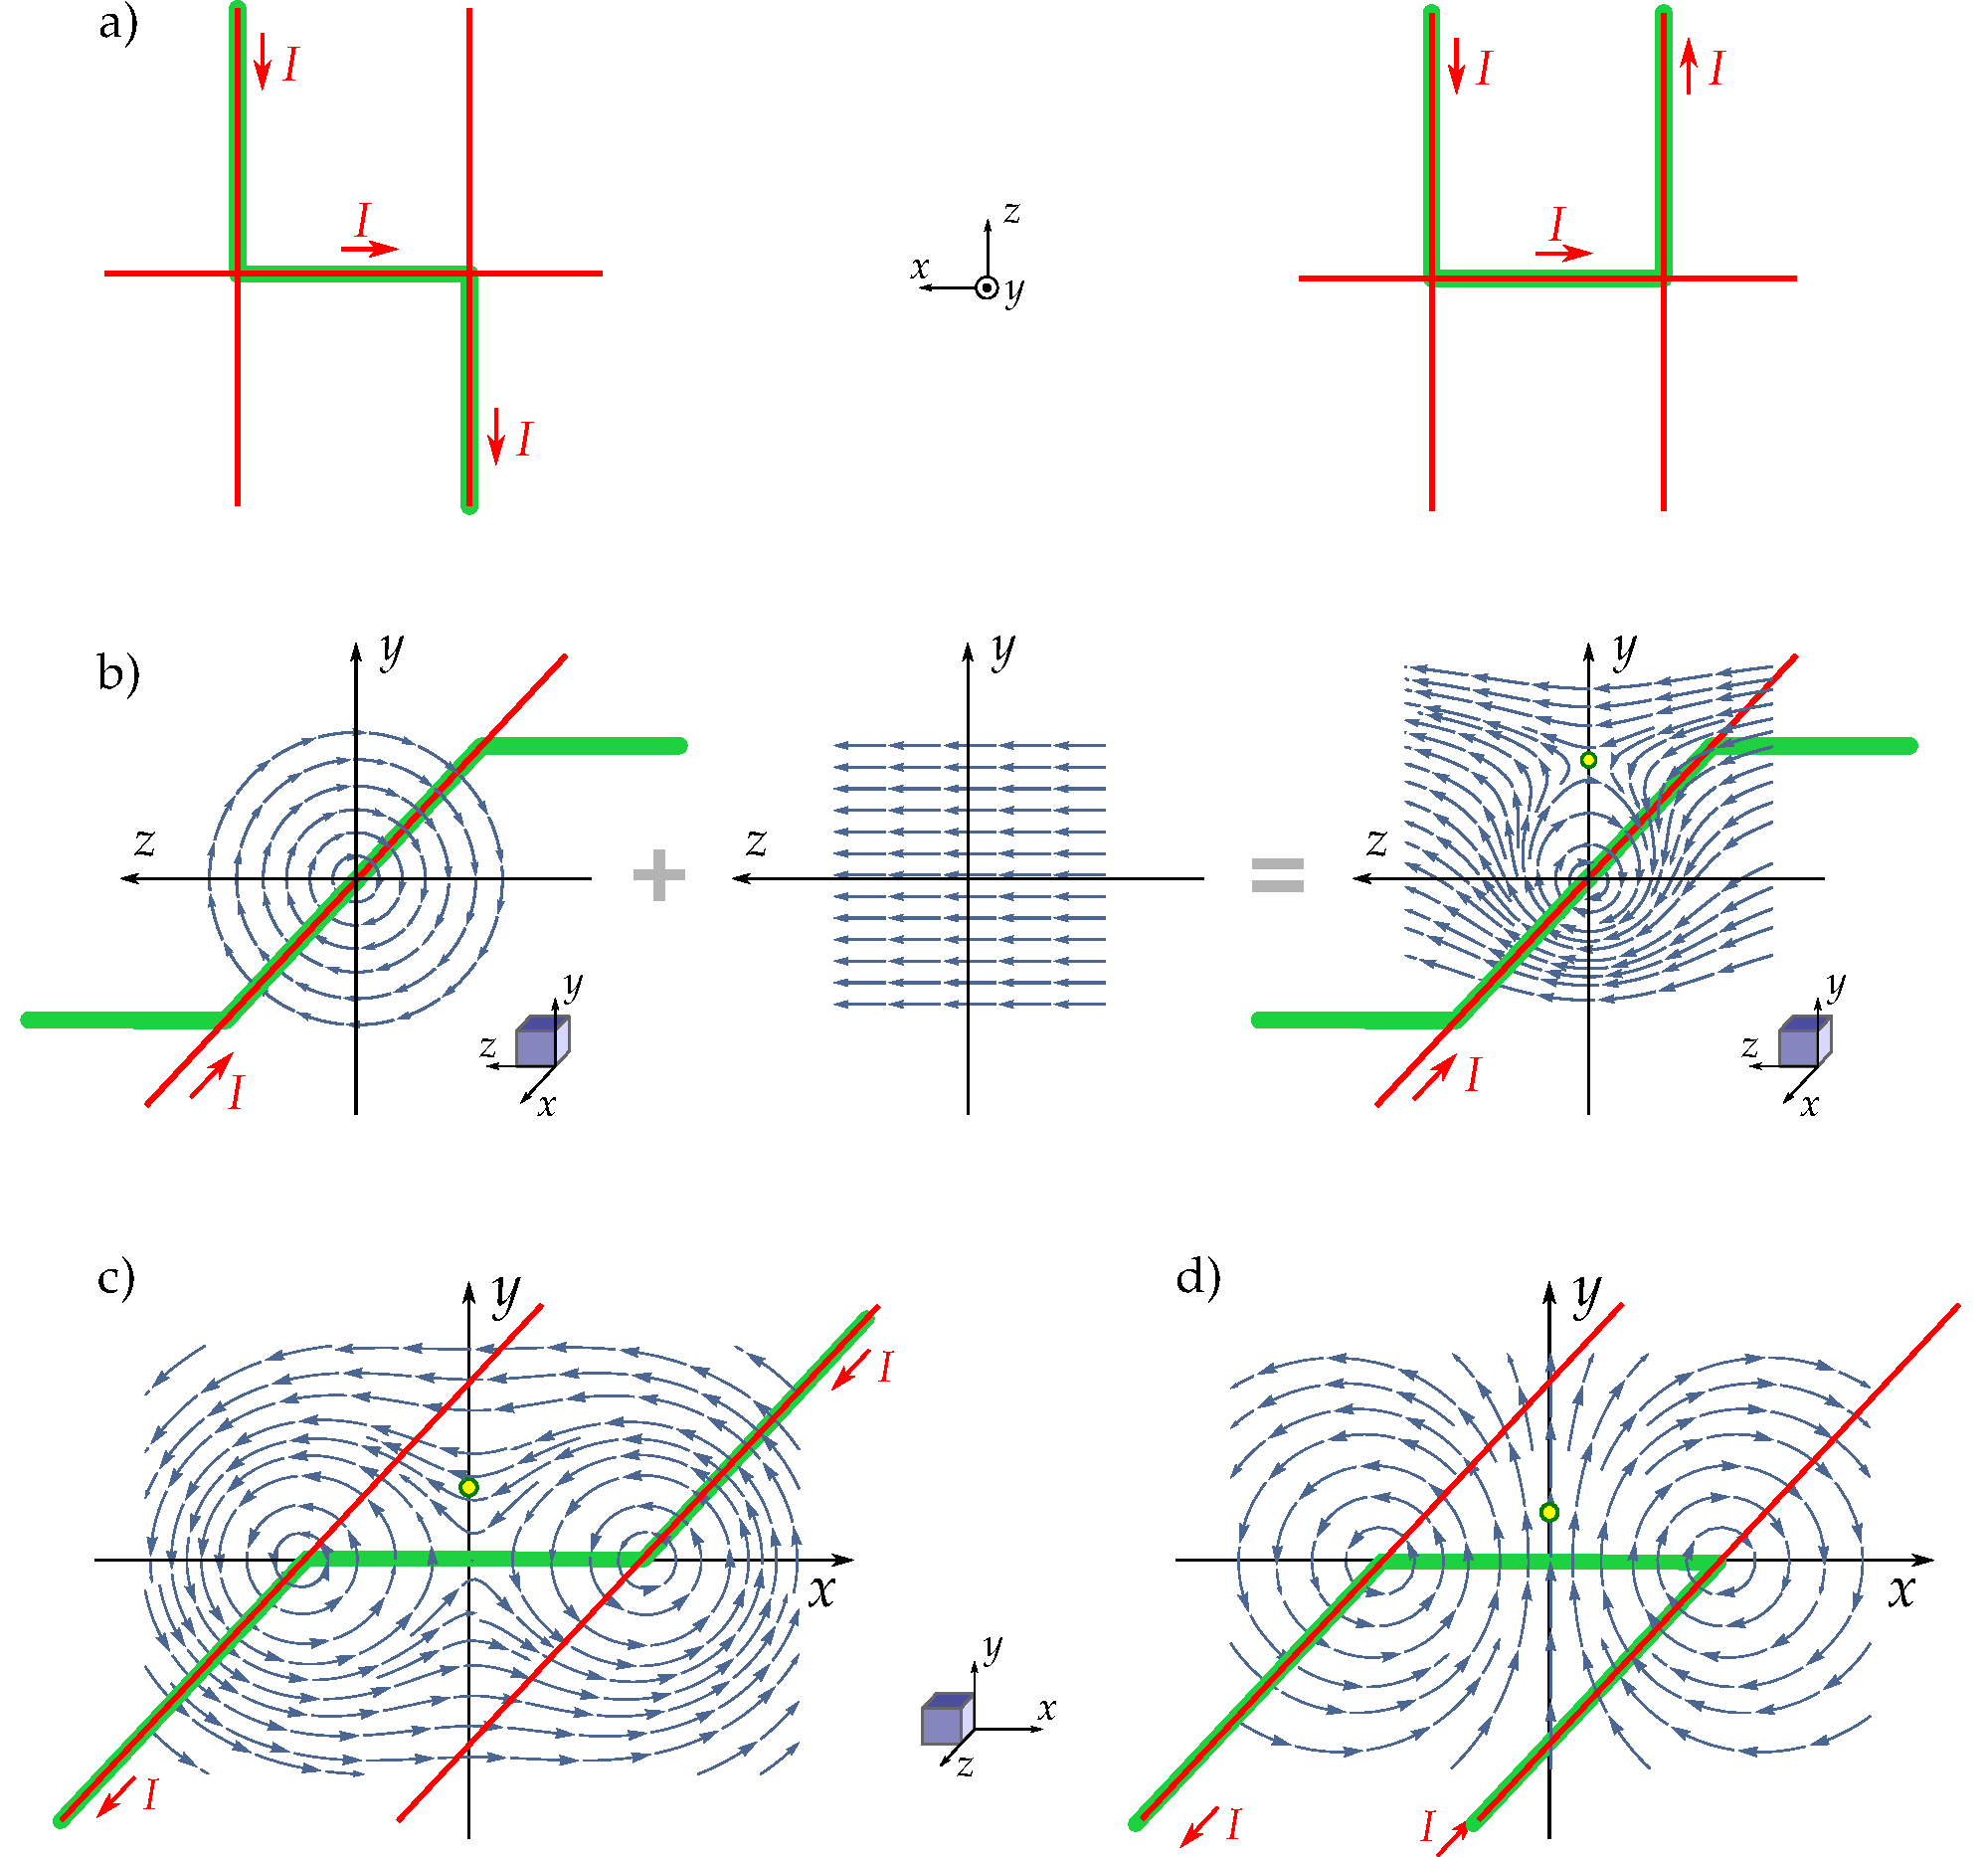
\includegraphics[width=\linewidth]{figures/setup/coldatoms/magfields_chip}
\caption[Champs magnétiques créés par la puce]{
Champs magnétiques créés par la puce.
\textbf{a)} Les fils \mcal{U} et \mcal{Z} portent un courant dans la direction $x$ et une paire de courants parallèles dans la direction $z$.
\textbf{b)} Un champ quadrupolaire est créé par la superposition du courant selon $x$ et d'un champ de biais $B_Z$.
Les courants verticaux peuvent circuler soit (\textbf{c)}) dans le même sens,  soit (\textbf{d)}) dans des sens opposés.
Le module du champ total présente alors respectivement un minimum non-nul ou nul aux positions marquées par les points jaunes.
}
\label{fig:magfields_chip}
\end{figure}

Pour le fil en \mcal{Z} comme pour le fil en \mcal{U}, le centre du piège se situe à une distance de la puce valant approximativement
\begin{equation}
\label{eq:trap_center}
r_0 \simeq \frac{\mu _0}{2\pi}\frac{I}{B_Z}
\end{equation}
et le gradient de champ magnétique à cet endroit vaut
\begin{equation}
\label{eq:trap_center_grad}
|B'(r_0)|=\frac{2\pi}{\mu _0} \frac{B_Z^2}{I} = \frac{B_Z}{r_0} = \frac{\mu _0}{2\pi}\frac{I}{r_0^2}~.
\end{equation}
%
C'est là une caractéristique importante de la géométrie des pièges : plus le centre du piège est proche de la puce, plus le piège sera confinant dans le plan $yz$.
Le piège s'allonge alors dans la direction $x$, prenant une forme de cigare de plus en plus anisotrope.

\clearpage
Comme nous l'avons mentionné, notre dispositif nous permet de mettre en \oe uvre des pièges magnéto-optiques en trois dimensions.
Dans beaucoup d'expériences d'atomes froids, ceux-ci sont réalisés à l'aide de trois paires de faisceaux laser contra-propageants, une dans chaque direction de l'espace.
Il nous est impossible d'envisager cette configuration, puisque l'axe $y$ est rendu inaccessible par la présence de la puce.
L'on peut cependant, avec deux paires de faisceaux laser seulement, simuler une configuration à six faisceaux, en utilisant la surface réfléchissante de la puce.
Deux faisceaux sont alors envoyés parallèlement à la surface de la puce, selon l'axe $x$.
Deux autres faisceaux sont envoyés dans le plan $yz$ et viennent se réfléchir sur la puce avec un angle de $\SI{45}{\degree}$.
Ces réflexions sont équivalentes aux deux faisceaux manquants, réalisant ainsi la configuration à six faisceaux souhaitée.
Le schéma de cette configuration, appelée \og MOT miroir \fg{}, est donné en figure \eqref{fig:mirror_MOT}.

\begin{figure}[h]
\centering
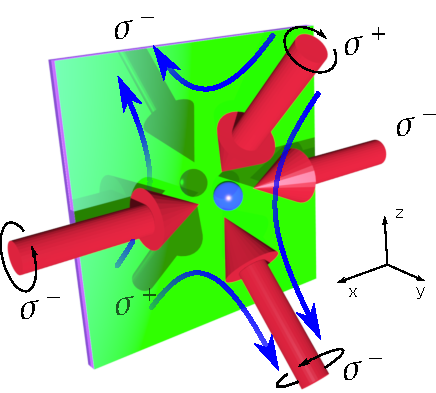
\includegraphics[width=0.6\linewidth]{figures/setup/coldatoms/mirror_MOT}
\caption[Schéma de principe du MOT miroir]{Schéma de principe du MOT miroir :
Deux faisceaux contra-propageants sont envoyés parallèlement à la puce réfléchissante, selon l'axe $x$.
Les deux autres faisceaux dans le plan $yz$ viennent frapper la puce avec un angle de \SIvv{45}{\degree}.
Leur réflexion sur la puce équivaut à deux faisceaux supplémentaires d'hélicité inversée, représentés en ombre derrière la puce.
On obtient bien ainsi une configuration de MOT à six faisceaux, avec les polarisations adaptées, représentées par des flèches tournant autour des faisceaux.
}
\label{fig:mirror_MOT}
\end{figure}


%\clearpage
\subsection{Séquence de piégeage et refroidissement}\label{subsec:exp_seq}
\noindent Grâce à ce dispositif, nous pouvons piéger des nuages d'atomes froids sur puce.
Nous donnons dans ce paragraphe le détail des différentes étapes de piégeage et de refroidissement des atomes.
Les atomes sont envoyés dans le cryostat à partir d'un piège magnéto-optique à deux-dimensions externe, puis ils sont capturés dans deux pièges magnéto-optiques sur puce successifs.
Enfin, les atomes sont transférés dans un piège magnétique pour y être refroidis par évaporation.
L'ensemble de cette séquence est représentée en figure \ref{fig:exp_sequence}.
%	
\begin{sidewaysfigure}
\centering
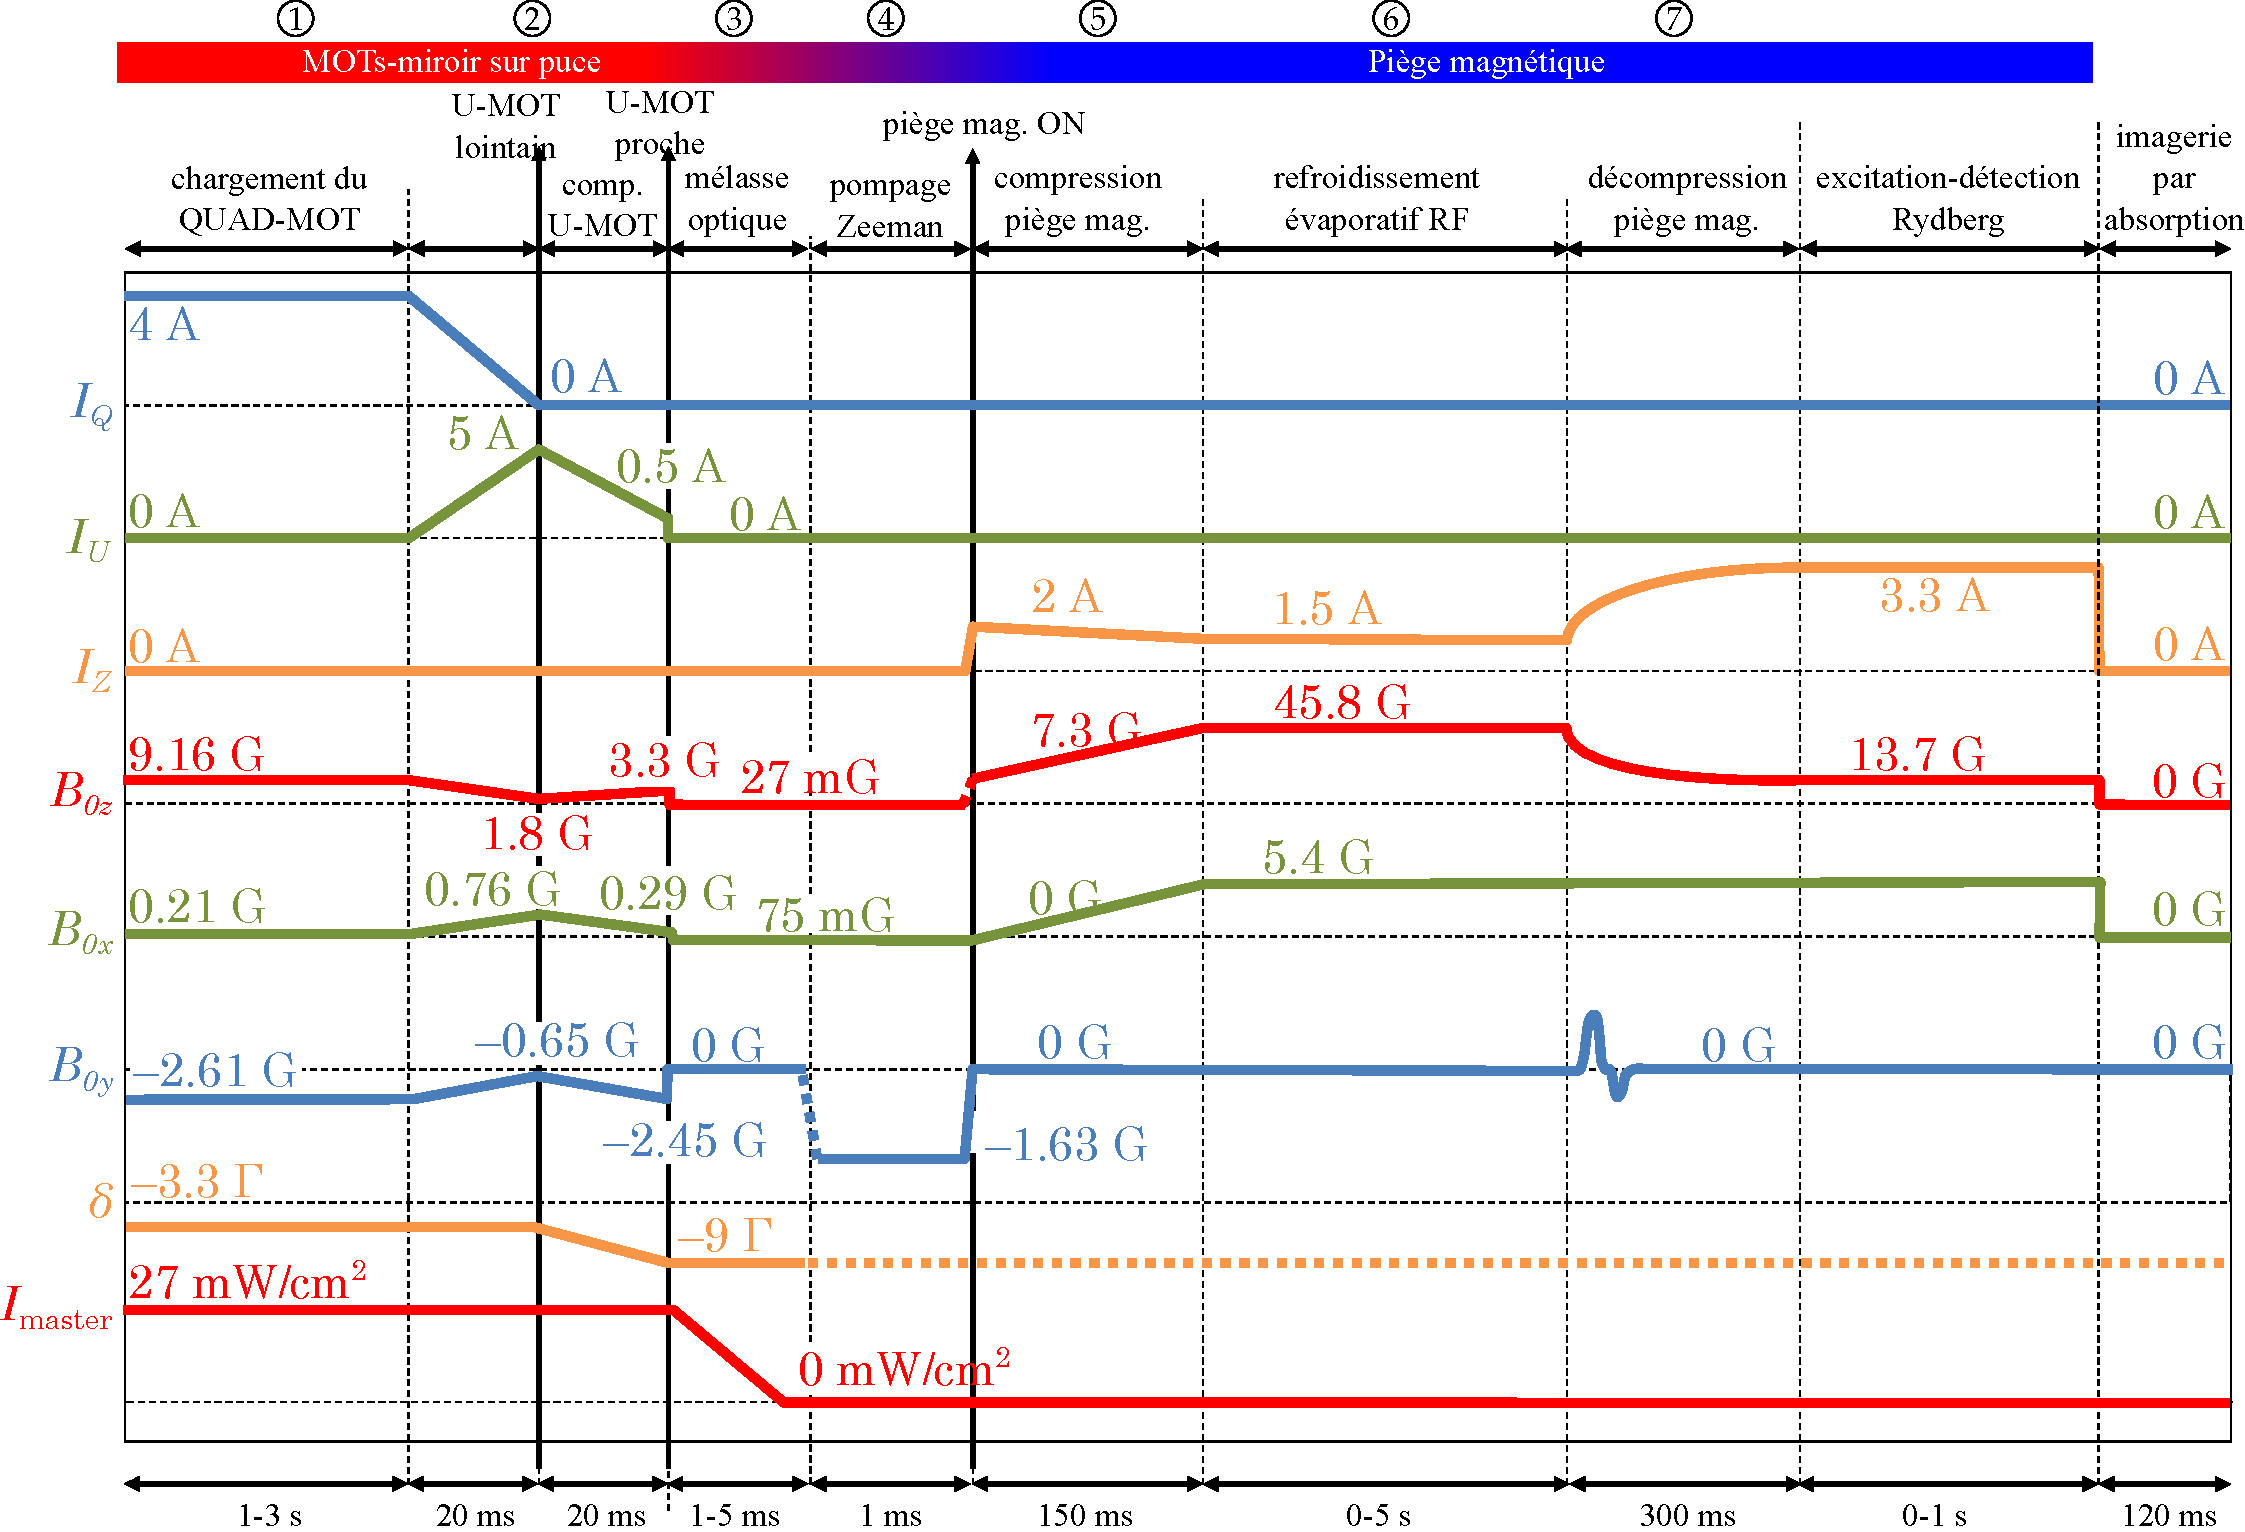
\includegraphics[width=\linewidth]{figures/setup/coldatoms/exp_sequence}
\caption[Séquence expérimentale typique]{Séquence expérimentale typique.% : la durée et les valeurs des paramètres à chaque étape sont précautionneusement optimisés.
Les étapes de piégeage et de refroidissement sont %numérotées de \numrange{1}{7} et 
discutées dans le texte.
Les étapes ultérieures seront décrites par la suite.
$I_{Q,U,Z}$ sont les courants dans la bobine QUAD, le fil \mcal{U} et le fil \mcal{Z}, en Ampères.
$B_{0~x,y,z}$ sont les champs de biais générés par les bobines dans les directions $x,y,z$, en Gauss.
$\delta$ est le désaccord du laser en unité de la largeur de raie $\Gamma=\SI{6.065}{\MHz}$, et $I_{master}$ son intensité en \si[per-mode=symbol]{\milli\watt \per\squared\cm}.
}
\label{fig:exp_sequence}
\end{sidewaysfigure}


\clearpage
\subsubsection*{Système laser}
\noindent Le piégeage magnéto-optique du rubidium 87 exploite la raie D2 de celui-ci.
La raie D2 est représentée en figure \eqref{fig:D2lineRb87} avec le détail des sous-niveaux hyperfins des niveaux $\mathrm{5S_{1/2}}$ et $\mathrm{5P_{3/2}}$ du \Rb{87}.
%	
\begin{figure}[t]
\centering
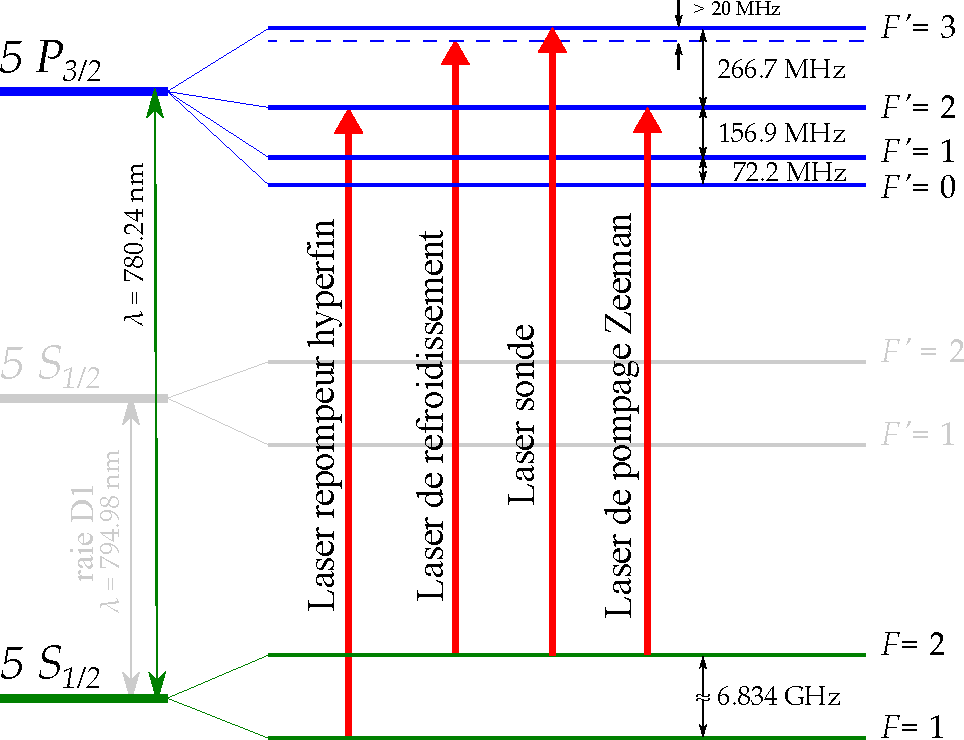
\includegraphics[width=0.8\linewidth]{figures/setup/coldatoms/D2lineRb87}
\caption[Raie D2 du \Rb{87}]{Structure hyperfine de la raie D2 du \Rb{87}.
Les transitions cyclantes sont montrées pour le laser de refroidissement, le laser repompeur, le laser sonde et le laser de pompage Zeeman.
}
\label{fig:D2lineRb87}
\end{figure}
%
Nous utilisons la transition $\ket{F=2} \rightarrow \ket{F'=3}$ de la raie D2 pour piéger et refroidir les atomes.
Cette transition a une largeur naturelle $\Gamma = 2\pi \times \SI{6.065}{\MHz}$ \cite{DATA_STECKRB87}.
Le laser de refroidissement est généré par un système commercial de diode laser amplifiée TOPTICA TA 100.
La fréquence de ce laser est asservie par battement (\og beatlock \fg{}) à un laser maître, lui-même stabilisé par une cavité Fabry-Pérot.
Cette cavité est verrouillée en fréquence sur la transition de refroidissement par absorption saturée dans une cellule de \Rb{87}.
Une commande de tension permet de définir la fréquence du battement et ainsi de contrôler le désaccord du laser de refroidissement par rapport à la transition $\ket{F=2}\rightarrow\ket{F'=3}$.
Le système de stabilisation et de distribution des faisceaux laser de piégeage et de refroidissement est détaillé en annexe \ref{app:laserlock}.

Il arrive qu'un photon du laser de refroidissement excite un atome du niveau $\ket{F=2}$ vers le niveau $\ket{F'=2}$ au lieu de $\ket{F'=3}$.
Cet atome peut alors se désexciter non pas vers le niveau $\ket{F=2}$ mais vers le niveau $\ket{F=1}$, qui est un niveau noir pour le laser de refroidissement.
Afin d'éviter le pompage des atomes vers ce niveau $\ket{F=1}$, il est nécessaire d'envoyer, avec le laser de refroidissement, un laser \og repompeur\fg{} accordé sur la transition $\ket{F=1}\rightarrow \ket{F'=2}$.
Ce laser repompeur est généré par une troisième diode laser, et indépendamment verrouillé en fréquence par absorption saturée.

Deux autres fréquences laser sont utilisées dans notre expérience : les lasers de sonde, qui servent à l'imagerie atomique, et le laser de pompage Zeeman, qui sert à réaliser un pompage optique vers le niveau $\ket{F=2,m_F=+2}$.
Ces faisceaux sont prélevés sur le laser de refroidissement et décalés en fréquence par modulation acousto-optique.
L'ensemble des faisceaux est transporté de la table optique de préparation au cryostat par des fibres optiques mono-modes à maintien de polarisation.
Ils sont enfin mis en forme à proximité immédiate du cryostat. 


%\clearpage
\subsubsection*{Piégeage magnéto-optique}
\noindent	Notre dispositif repose sur trois stades de piégeage magnéto-optique successifs.
Les atomes de rubidium sont stockés dans une cellule en verre, ouverte vers une enceinte sous ultra-vide (UHV) située à l'extérieur du cryostat.
Le travail en environnement cryogénique nous oblige en effet à utiliser une source externe : l'adsorption sur les surfaces froides à l'intérieur du cryostat interdit la présence d'une vapeur de rubidium à partir de laquelle capturer les atomes.
Dans cette enceinte, les atomes sont piégés le long de l'axe $z$ par un piège magnéto-optique à deux dimensions (\og 2D-MOT \fg{}).
Celui-ci est schématisé en figure \eqref{fig:2DMOT}.
L'ensemble du 2D-MOT a été conçu et fabriqué par le laboratoire SYRTE de l'Observatoire de Paris.
%	
\begin{figure}[h]
\centering
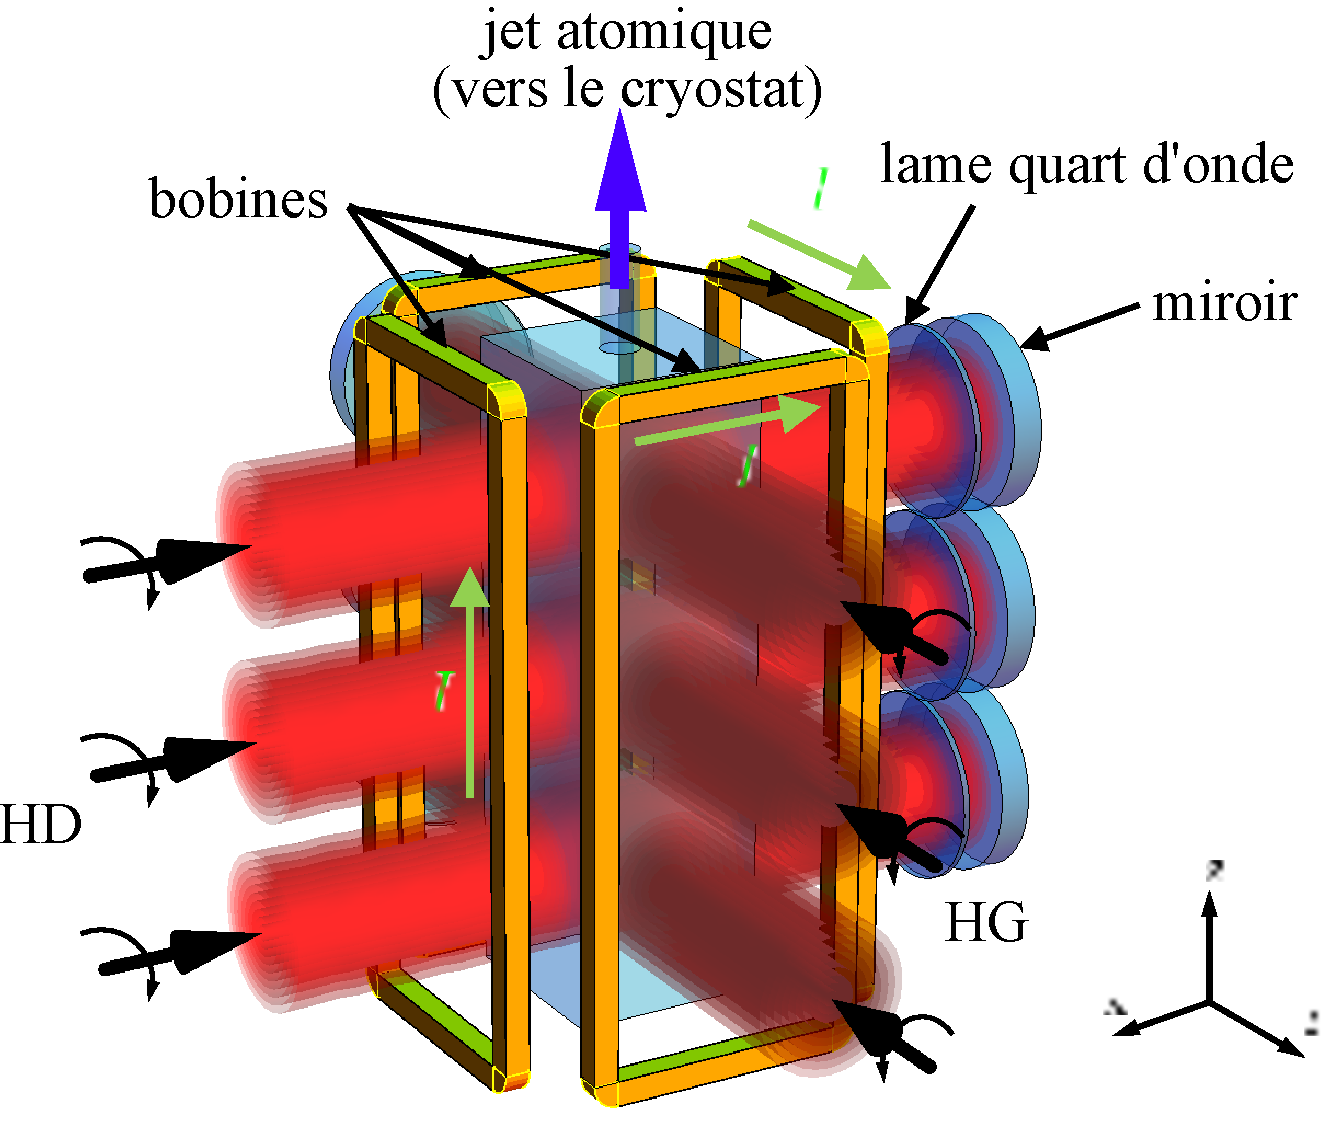
\includegraphics[width=0.6\linewidth]{figures/setup/coldatoms/2DMOT_2}
\caption[Schéma du 2D-MOT]{Schéma du 2D-MOT avec ses trois étages de piégeage.
Les polarisations des faisceaux incidents sont indiquées par les lettres HD (pour hélicité droite) et HG (hélicité gauche).%, relativement à la direction de propagation des faisceaux.
Le sens des courants dans les bobines est indiqué par les flèches vertes et la lettre $I$.
Chaque faisceau est rétro-réfléchi par un miroir, et le double passage par une lame quart d'onde permet de garantir la bonne polarisation du faisceau réfléchi.
Le jet atomique produit par le 2D-MOT est représenté par une flèche violette qui pointe vers le cryostat.
}
\label{fig:2DMOT}
\end{figure}
%

Les atomes piégés dans le 2D-MOT se propagent librement selon l'axe $z$, formant un jet vertical qui arrive jusqu'à la puce atomique à l'intérieur du cryostat.
Les atomes sont alors capturés dans un MOT de grand volume créé par les bobines de biais et le bas de la bobine \og QUAD \fg{}, représentée en figure \eqref{fig:cryo}.
Le bas de la bobine QUAD permet de créer un champ quadrupolaire similaire à celui du fil \mcal{U}, adapté au piégeage magnéto-optique.
Le nombre de spires $n=19$ de la bobine permet de multiplier par autant le courant générateur de champ dans l'équation \eqref{eq:trap_center}.
Le grand volume du champ quadrupolaire ainsi créé permet de capturer efficacement les atomes du jet.
Le chargement de ce gros \og QUAD-MOT \fg{} dure de \SIvv{1}{} à \SIvv{3}{\s}, pendant lesquels on peut y collecter quelques \SIvv{e8} atomes à une température de l'ordre de \SIvv{400}{\uK}.

Le nuage atomique est alors transféré vers un second MOT, créé cette fois par les bobines de biais et le fil \mcal{U}, comme nous l'avons mentionné en \ref{subsec:cryopuce}.
Ce \og U-MOT lointain\fg{} présente des gradients similaires au QUAD-MOT mais un volume plus petit.
Le taux de transfert entre les deux est estimé entre $\num{10}$ et $\SI{40}{\percent}$ par des observations en fluorescence du nuage.
Nous pouvons à ce moment réduire le courant dans le fil \mcal{U}, ce qui d'après les équations \eqref{eq:trap_center} et \eqref{eq:trap_center_grad} rapproche le piège de la surface de la puce et le comprime en augmentant les gradients de champ magnétique.
Les gradients de champ étant plus forts, la force de rappel de la lumière s'en trouve grandie.
On peut alors se permettre d'augmenter le désaccord des faisceaux lasers afin de refroidir le nuage atomique.
Les températures atteintes dans ce \og U-MOT proche\fg{} sont de l'ordre de $\SI{40}{\uK}$, pour un nuage d'environ $\numrange{e7}{e8}$ atomes.

%\clearpage
\subsubsection*{Les étapes intermédiaires : mélasse optique et pompage Zeeman}
\noindent L'objectif, après les étapes de piégeage magnéto-optique, est de transférer les atomes dans le piège de Ioffe-Pritchard créé par le fil \mcal{Z}.
Cela sera d'autant plus efficace que le nuage atomique sera froid, et que les atomes seront bien polarisés dans le sous-niveau Zeeman $m_F=+2$ du niveau hyperfin $\mathrm{5S1/2,F=2}$.
Avant de les transférer vers le \og piège Z \fg{}, nous faisons donc subir aux atomes deux étapes supplémentaires.

Tout d'abord, nous éteignons les champs magnétiques du U-MOT en laissant les faisceaux lasers allumés.
Cela initie une étape de mélasse optique d'une durée comprise entre $\num{1}$ et $\SI{5}{\ms}$, au cours de laquelle le désaccord laser est augmenté alors que la puissance lumineuse est graduellement diminuée jusqu'à zéro.
Cette mélasse optique nous permet de refroidir quelques $\numrange{e6}{e7}$ atomes à des températures inférieures à $\SIvv{10}{\uK}$.

Après l'extinction des lasers de mélasse, un champ magnétique de \SIrange{1}{2}{\gauss} est rapidement allumé sur la direction $-y$, qui lève la dégénérescence des sous-niveaux Zeeman.
Un laser de pompage optique polarisé $\sigma ^+$ se propageant selon $-y$ pompe alors les atomes dans le sous-niveau $m_F=+2$.
Après réflexion sur la puce ce faisceau laser repasse à travers le nuage atomique.
Son hélicité a certes été inversée par la réflexion, mais sa polarisation du point de vue des atomes est restée la même.
Les atomes sont donc encore pompés vers le sous-niveau $m_F=+2$.

%\clearpage
\subsubsection*{Le piégeage magnétique et le refroidissement évaporatif}
\noindent Lorsque le nuage atomique est bien refroidi et polarisé par les étapes de mélasse et de pompage optique, le piège magnétique est allumé.
Pour cela, un courant est imposé dans le fil \mcal{Z}.
Un champ $B_z$ est généré par les bobines, qui permet d'obtenir un champ quadrupolaire comme nous l'avons évoqué en \ref{subsec:cryopuce}, centré sur la position du nuage atomique.
Le champ au centre du piège est alors orienté selon la direction $x$ et le minimum de champ, strictement supérieur à $0$, permet d'éviter les pertes de Majorana par retournement du spin.
Un second champ de biais, $B_x$, permet en outre de limiter les pertes atomiques dues à la présence d'un bruit radio-fréquence dans notre expérience.
Ce bruit peut en effet causer des transitions atomiques vers les états non piégés $m_F<1$ et il s'agit d'ajuster $B_x$ afin d'éviter que les transitions ne soient résonantes avec la fréquence du bruit \cite{PHD_NIRRENGARTEN}.

Une fois allumé, le piège magnétique est immédiatement comprimé afin d'augmenter le taux de collision entre les atomes en vue du refroidissement évaporatif.
La compression du piège est réalisée adiabatiquement en \SI{150}{\ms}.
Le piège comprimé a des fréquences de piégeage de l'ordre de $(\omega_x,\omega_y,\omega_z) \simeq 2\pi \times (\num{24},\num{3400},\num{3400})~\si{\hertz}$ à une distance de \SI{80}{\um} de la puce.
Nous pouvons alors mettre en \oe uvre une séquence de refroidissement évaporatif radio-fréquence :
les atomes les plus chauds sont transférés vers les sous-niveaux Zeeman non piégés par des transitions radio-fréquence (RF), et ainsi sont éjectés du piège.
La fréquence de ces transitions dépend du champ magnétique vu par chaque atome, et donc de sa position dans le potentiel de piégeage.
La fréquence du signal RF, envoyé dans le fil vertical (KM) de la puce (cf figure \ref{fig:chip}), est progressivement diminuée afin d'évaporer les atomes les plus chauds en premier, puis de plus en plus froids.
Le reste du nuage thermalise vite grâce au taux de collision élevé et se trouve ainsi refroidi.
Plusieurs rampes de fréquence successives sont optimisées en durée et en puissance RF, afin d'obtenir le meilleur refroidissement du nuage atomique.
L'étape de refroidissement évaporatif dure jusqu'à \SI{5}{\second} au total.
Le schéma de principe du refroidissement évaporatif RF est donné en figure \eqref{fig:evapRF}.
%
\begin{figure}[!h]
\centering
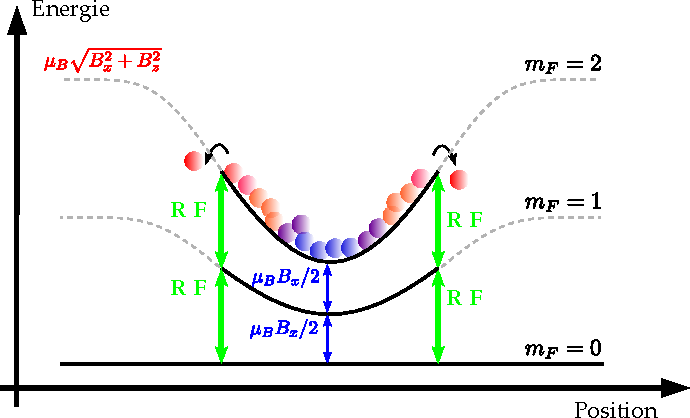
\includegraphics[width=.7\linewidth]{figures/setup/coldatoms/evapRF}
\caption[Refroidissement évaporatif RF]{Refroidissement évaporatif radio-fréquence :
le \og couteau \fg{} RF induit les transitions entre sous-niveaux Zeeman.
Une fois dans les sous-niveaux $m_F<1$, les atomes ne sont plus piégés et sont éjectés du piège.
L'aile chaude de la distribution de Boltzmann est évacuée et les atomes restant sont thermalisés à une température plus faible.
}
\label{fig:evapRF}
\end{figure}

Cette étape de refroidissement nous permet d'abaisser la température du nuage sous le seuil de condensation de Bose-Einstein.
Nous pouvons ainsi produire de façon reproductible des condensats sur puce contenant de \SIrange{10000}{20000}{} atomes.
La séquence de refroidissement peut également être interrompue avant la condensation, et en choisissant la fréquence finale de la rampe RF, nous pouvons choisir la température du nuage atomique.
La figure \eqref{fig:BEC} montre des images du nuage atomique après temps de vol pour différentes valeurs de la fréquence finale de la rampe RF.
%
\begin{figure}[!h]
\centering
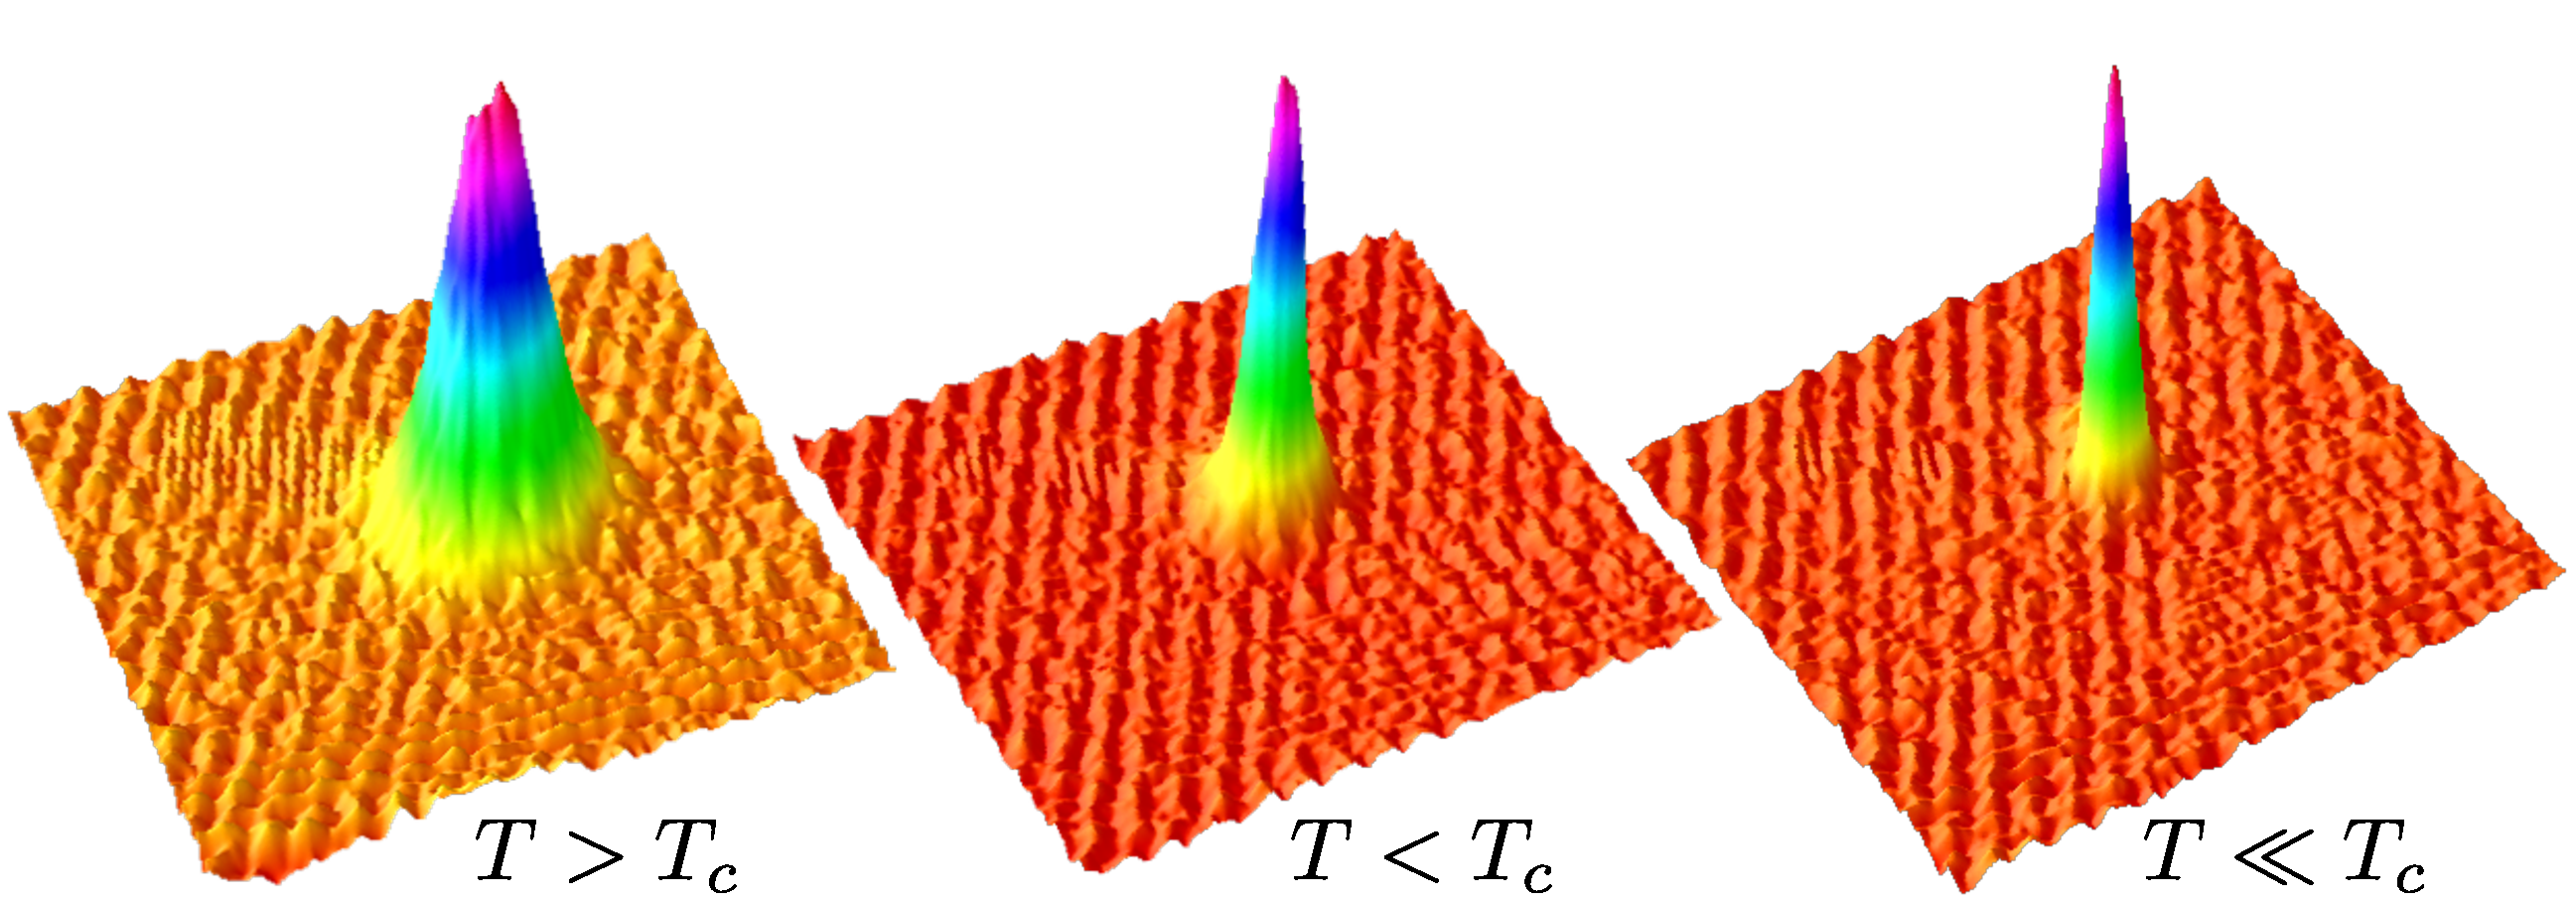
\includegraphics[width=.8\linewidth]{figures/setup/coldatoms/BEC}
\caption[Condensat de Bose-Einstein sur puce]{
Trois nuages de \Rb{87} évaporés jusqu'à des valeurs différentes de fréquence RF, imagés après un temps de vol de \SI{16.5}{\ms}.
Les images donnent directement la distribution d'impulsion au sein du nuage.
Le nuage contient environ $\SI{e4}{}$ atomes, et la tepérature critique de condensation est de l'ordre de $T_C = \SI{100}{\nano\K}$.
\`A gauche, la température est supérieure à $T_C$: le nuage est purement thermique et montre une distribution gaussienne d'impulsion.
Au milieu, la température est inférieure à $T_C$, le nuage montre un double profil en impulsion : un condensat de Bose-Einstein au centre et les atomes du nuage thermique autour.
\`A droite, la température est très petite devant $T_C$ et le condensat est quasi-pur : le nuage présente un profil de Thomas-Fermi dans l'espace des impulsions.
}
\label{fig:BEC}
\end{figure}
%

Enfin, une fois le nuage refroidi à la température souhaitée, le piège magnétique est décomprimé.
Cela permet de choisir soit une distance particulière du nuage atomique à la puce, soit la taille du nuage atomique final.

Les atomes qui seraient restés dans le sous-niveau $m_F=+1$ peuvent à leur tour être éliminés du piège en envoyant sur le nuage un signal micro-onde à \SI{6.8}{\GHz} adressant la transition hyperfine $\ket{F=2,m_F=1} \rightarrow \ket{F=1,m_F=0}$.
En présence d'un champ magnétique, les sous-niveaux Zeeman sont suffisamment résolus pour adresser uniquement cette transition, sans affecter les atomes dans le niveau $\ket{F=2,m_F=+2}$.

%\clearpage	
\subsection{Imagerie atomique par absorption}
\noindent Dans une expérience d'atomes froids, il est essentiel de pouvoir imager et dénombrer correctement le nuage atomique.
L'imagerie par absorption est une technique précise et efficace pour cela.
%Elle consiste à envoyer sur les atomes un faisceau laser, résonnant avec une transition atomique choisie, et à mesurer quelle fraction de la lumière le nuage atomique a absorbé.
Lorsqu'une telle expérience est menée au c\oe ur d'un cryostat, la tâche est rendue plus difficile en raison des accès optiques limités qui contraignent fortement l'optique d'imagerie.

\subsubsection*{Dispositif optique}
\noindent Nous pouvons imager notre nuage atomique de deux façons différentes.
Le dispositif optique d'imagerie est représenté en figure \eqref{fig:probes_CdF}.

Un premier faisceau sonde (\og sonde face \fg{})  entre dans le cryostat et en ressort perpendiculairement à la puce après réflexion sur celle-ci, par le hublot de face.
Un miroir percé permet de laisser passer le faisceau d'entrée et de collecter le faisceau de sortie, qui est ensuite envoyé vers une caméra CCD.
Grâce à l'installation d'une lentille de focale $f=\SI{100}{\mm}$ à la place du hublot de face sur la jupe hélium du cryostat, soit à environ $\SI{100}{\mm}$ de la puce, cet axe d'imagerie peut collecter beaucoup de lumière, avec une limite de résolution de $\SI{1.6}{\um}$.

Un deuxième faisceau sonde (\og sonde côté \fg{}) est envoyé par un hublot de côté ($+x$), se réfléchit sur la puce avec un angle de \SIrange{5}{10}{\degree}, et ressort par l'autre hublot de côté ($-x$). Il est ensuite envoyé vers une autre caméra CCD.
Cet axe d'imagerie ne dispose pas d'une lentille interne au cryostat. Ainsi, la lumière collectée et la résolution optique sont limitées par le diamètre du hublot de sortie du cryostat.
%le diamètre de la première lentille après la sortie du cryostat.
Cette lentille est donc placée le plus près possible de l'enceinte du cryostat.
En raison de cette géométrie, l'imagerie des atomes par la sonde côté forme deux images du nuage atomique : celui absorbe à la fois le faisceau incident et le faisceau réfléchi sur la puce.
Cela nous permet d'évaluer précisément la distance du nuage atomique à la puce : elle vaut la moitié de la distance entre les deux images du même nuage.
La figure \eqref{fig:double_cloud} montre une image d'absorption de la sonde côté par un nuage froid (piégé magnétiquement et refroidi), après un temps de vol de \SI{16.5}{\ms}.

\begin{figure}[h]
\centering
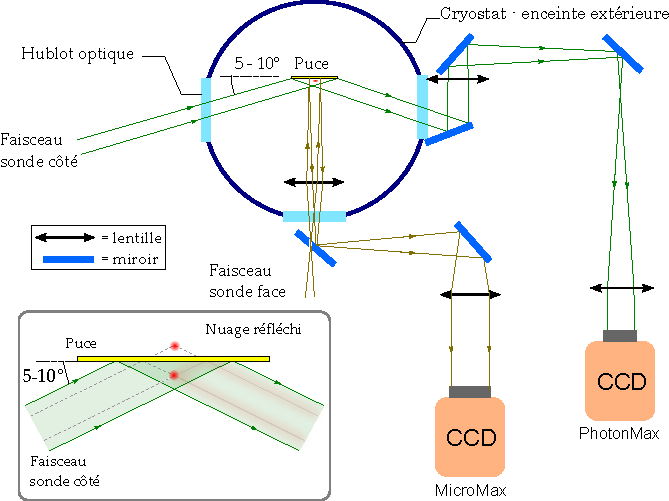
\includegraphics[width=.7\linewidth]{figures/setup/coldatoms/probes_CdF}
\caption[Faisceaux sonde]{Schéma optique des faisceaux sonde dans le cryostat.
L'insert montre de plus près la réflexion du faisceau sonde côté sur la puce et la formation des deux images du nuage.
}
\label{fig:probes_CdF}
\end{figure}

\begin{figure}[h]
\centering
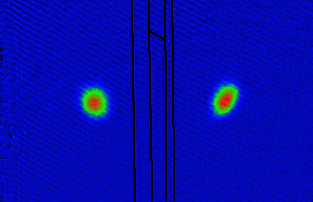
\includegraphics[width=.6\linewidth]{figures/setup/coldatoms/double_cloud_withWires}
\caption[Image par absorption du nuage par la sonde côté]{Image par absorption d'un nuage froid après temps de vol, éclairé par la sonde de côté. Les deux images du nuage sont dues à la réflexion du faisceau sur la puce.
Les ombres portées des fils de la puce sont tracées en surimpression entre les deux images du nuage.
}
\label{fig:double_cloud}
\end{figure}

%\clearpage
\subsubsection*{Principe de l'imagerie par absorption}
\noindent Les atomes peuvent être observés en temps réel par la collecte des photons qu'ils émettent par fluorescence, mais l'imagerie par absorption permet une meilleure précision sur l'estimation du nombre d'atome dans le nuage.
Elle consiste à envoyer sur les atomes un faisceau laser, résonant avec une transition atomique choisie, et à mesurer quelle fraction de la lumière le nuage atomique a absorbé.

Lorsque l'intensité lumineuse reçue par les atomes est largement inférieure à l'intensité de saturation, l'absorption de celle-ci est bien décrite par la loi de Beer-Lambert :
\begin{equation}
\label{eq:Beer-Lambert}
\frac{dI(x,y,z)}{dx} = -\sigma n(x,y,z) I(x,y,z),
\end{equation}
où $I(x,y,z)$ est l'intensité lumineuse au point de coordonnées $(x,y,z)$, $n$ la densité atomique en ce point, $x$ la direction de propagation du faisceau lumineux et $\sigma$ la section efficace de diffusion de la lumière par un atome unique.
L'optique d'imagerie nous oblige cependant à intégrer cette équation dans la direction de propagation $x$.
On obtient alors 
\begin{equation}
\label{eq:Beer-Lambert_integ}
I_f(y,z) = I_i (y,z)\cdot e^{-\int dx~\sigma~n(x,y,z)}
\end{equation}
où $I_i$ est l'intensité du faisceau incident et $I_f$ l'intensité du faisceau à la sortie du nuage atomique.

Les images enregistrées par les caméras permettent d'obtenir les quantités $I_i(y,z)$ et $I_f(y,z)$.
On peut alors calculer la densité optique du nuage , définie comme $OD(y,z) = \int dx~\sigma~n(x,y,z)$, et qui d'après l'équation \eqref{eq:Beer-Lambert_integ} est égale à
\begin{equation}
\label{eq:OD}
OD(y,z) = \int dx~\sigma~n(x,y,z) = -\ln \frac{I_f(y,z)}{I_i(y,z)}.
\end{equation}
L'on en extrait ensuite la densité atomique intégrée le long de l'axe de propagation du laser à partir de l'équation \eqref{eq:OD} :
\begin{equation}
\label{eq:atomic_density}
n(y,z) = \int{dx~n(x,y,z)} = -\frac{1}{\sigma} \ln \frac{I_f(y,z)}{I_i(y,z)} = \frac{OD(y,z)}{\sigma}.
\end{equation}
		
Dans le cas simple d'une lumière résonante avec la transition non-dégénérée d'un système à deux niveaux, la section efficace de diffusion $\sigma$ est donnée directement par la section efficace de diffusion résonante 
\begin{equation}
\sigma = \sigma_0 = \frac{3\lambda^2}{2\pi} = \frac{\Gamma \hbar\omega}{2I_{sat,0}},
\end{equation}
où $\lambda$ est la longueur d'onde de la lumière résonante et $I_{sat,0}$ l'intensité de saturation de la transition dans ce cas idéal.
Les atomes dans notre piège magnétique sont préparés dans l'état $\ket{5S1/2,F=2,m_F=+2}$, et la lumière de sonde est préparée de façon à adresser la transition $\sigma^+$ vers le niveau $\ket{5P3/2,F=3,m_F=+3}$.

\clearpage
\subsubsection*{Corrections et améliorations de l'imagerie par absorption}
\noindent Malgré l'apparente simplicité du dispositif d'imagerie par absorption, plusieurs effets perturbent les mesures du nombre d'atomes et méritent d'être corrigés.

Premièrement, la section efficace de diffusion $\sigma$ dans notre expérience n'est pas égale à la section efficace de diffusion résonante $\sigma_0$.
En effet, la lumière des faisceaux sonde n'est pas parfaitement polarisée $\sigma^+$.
De plus, les atomes ne sont pas tous dans le sous-niveau $m_F=+2$, en particulier lorsque l'on souhaite imager le nuage dans le MOT ou après l'étape de mélasse optique sans le charger dans le piège magnétique.
Enfin, l'interférence entre le faisceau sonde de côté et sa réflexion sur la puce module l'intensité de la lumière vue par le nuage atomique.
La combinaison de ces effets réduit peut être décrite en corrigeant la section efficace de diffusion d'un facteur $\alpha$ \cite{PHD_CELISTRINO,MX_GUERYODELIN_SATABSIM}.
On obtient alors une section efficace de diffusion effective $\sigma = \sigma_0 / \alpha$, ou, de façon équivalente, une intensité de saturation effective $I_{sat} = \alpha\cdot I_{sat,0}$.
La calibration expérimentale de ce paramètre $\alpha$ est effectuée par la mesure de l'intensité de saturation effective $I_{sat}$.
Pour l'absorption de la sonde de côté par un nuage dans le piège magnétique, nous obtenons une valeur $\alpha_{magn} = \num{2.06} \pm \num{0.1}$.
Pour l'absorption de la sonde de côté par un nuage juste après la mélasse optique, nous obtenons une valeur $\alpha_{melasse} = \SI{2.27}{} \pm \SI{0.1}{}$.
Le nombre d'atomes évalué à partir des images par absorption dépend directement de la valeur de ce paramètre $\alpha$.
Les valeurs expérimentales proches de $\alpha=2$ sont tout à fait cohérentes avec le fait que notre faisceau sonde est polarisé linéairement : seule la composante $\sigma^+$ de la lumière résonante avec la transition sonde peut être absorbée.
Cette composante représente la moitié de l'intensité totale envoyée, et seule cette moitié contribue à la saturation de la transition.
Pour un même paramètre de saturation, l'intensité totale du faisceau doit donc être deux fois plus grande que si le faisceau était polarisé $\sigma^+$.
	
Deuxièmement, l'acquisition du signal d'imagerie se fait en trois temps.
Une première image est enregistrée où les atomes absorbent le faisceau sonde, ce qui nous donne l'intensité $I_f$.
Puis une deuxième image est enregistrée après que les atomes sont tombés par gravité, qui nous donne l'intensité du faisceau sonde non absorbé $I_i$.
Enfin, une troisième image est enregistrée sans aucun laser allumé, qui permet de soustraire la lumière de fond
%et le bruit électronique
des deux images précédentes.
Les délais de quelques dizaines de \si{\ms} entre les différentes images ont un effet délétère sur le signal.
En effet, le signal enregistré par la caméra subit un bruit d'imagerie sous la forme de franges, dues à la diffraction et aux interférences du faisceau laser le long de son chemin optique et lors de sa réflexion sur la surface de la puce.
Des vibrations et déformations de petite amplitude des éléments optiques et des variations d'indice de l'air le long du chemin optique décalent ces franges d'une image à l'autre.
L'opération de traitement des images (équation \ref{eq:atomic_density}) ne permet pas de d'affranchir des fluctuations de ces franges, qui viennent ainsi brouiller le signal d'imagerie.
%génèrent des franges dans les images traitées par l'équation \eqref{eq:atomic_density}, semblables à des franges d'interférence.
Ce problème se présente principalement sur l'imagerie par la sonde de face en raison des plus grands délais exigés par la caméra et de la plus grande sensibilité mécanique du chemin optique.
Afin d'y remédier, nous avons implémenté un algorithme de réduction des franges qui, à partir d'une base de plusieurs images du faisceau sonde seul, reconstitue la meilleure combinaison linéaire de celles-ci pour chaque image où le nuage atomique est présent. Cet algorithme est décrit en détail dans \cite{MX_WHITLOCK_FRINGEREDUCTION}.
La figure \eqref{fig:Fringe_Reduction} montre une image d'un nuage froid par absorption de la sonde face, non traitée et après traitement par cet algorithme.

\begin{figure}[h]
\centering
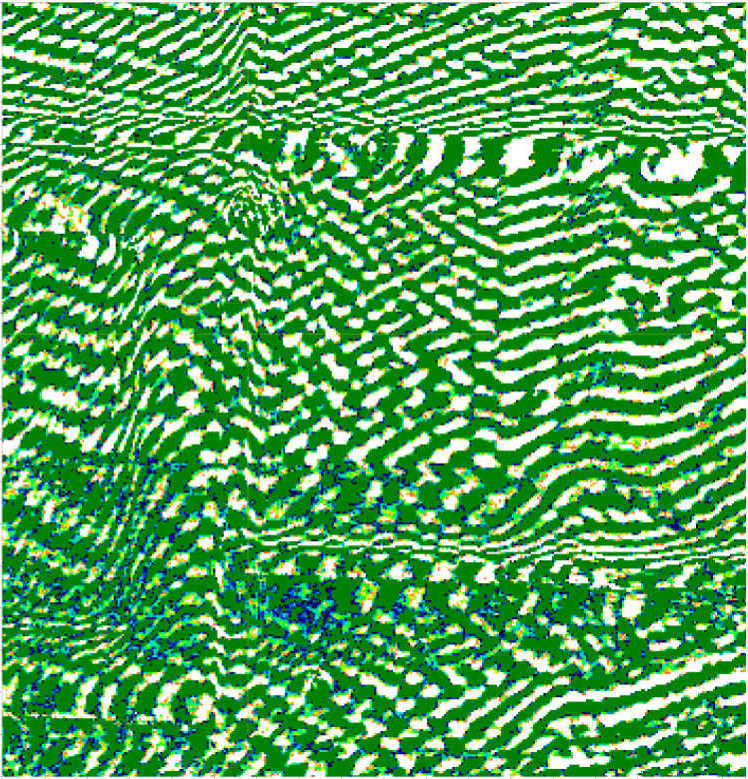
\includegraphics[width=0.35\linewidth]{figures/setup/coldatoms/Normal_abs2_onlyPic}
\hspace{.15\linewidth}
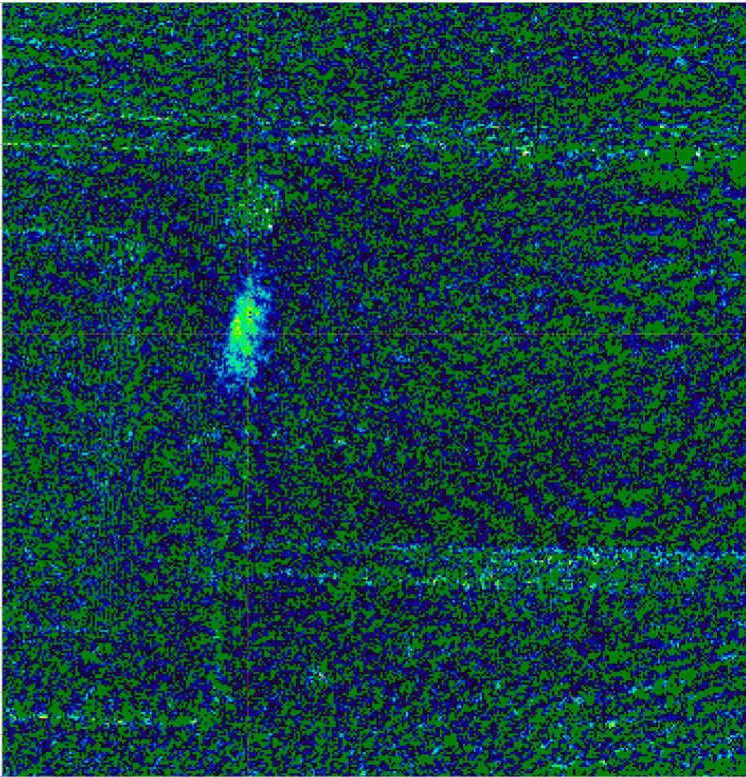
\includegraphics[width=0.35\linewidth]{figures/setup/coldatoms/RF_abs2_onlyPic}
\caption[Effet de l'algorithme de réduction des franges]{
Images du nuage atomique froid par absorption du faisceau sonde face.
\`A gauche, l'image est traitée selon l'équation \eqref{eq:atomic_density}.
\`A droite, la même image après traitement par l'algorithme de réduction des franges.
Les graphes sous les images sont les profils de densité du nuage en coupe horizontale.
L'échelle de couleur est la même pour les deux images et a été optimisée pour l'image de droite.
}
\label{fig:Fringe_Reduction}
\end{figure}

\newpage
Troisièmement, %il peut être intéressant, pour caractériser des nuages très denses, de ne pas calculer la densité optique $OD$ comme à l'équation \eqref{eq:Beer-Lambert_integ}.
%En effet, 
dans le cas d'un nuage très dense optiquement, comme par exemple pour les mélasses optiques, le centre du nuage où la densité atomique est très haute peut absorber l'intégralité de l'intensité incidente $I_i$.
Le rapport des intensités $I_f/I_i$ est alors très faible et dominé par le bruit.
Le signal $I_f/I_i$ au centre du nuage peut ainsi présenter des valeurs négatives, qui seront problématiques lorsque l'on souhaitera en prendre le logarithme.
%Or la valeur de la densité optique au centre du nuage est cruciale à l'ajustement de la densité à un profil gaussien.
Afin de remédier à cela, il peut être intéressant de ne pas calculer la densité optique $OD$ comme à l'équation \eqref{eq:Beer-Lambert_integ}, mais de s'arrêter à l'opération 
\begin{equation}
\label{eq:nolog_abs}
\frac{I_f(y,z)}{I_i(y,z)} = e^{-OD(x,y)} = e^{-\sigma .n(y,z)}.
\end{equation}
Nous appellerons cette opération \og absorption no-log \fg{}.
%Si le nuage présente un profil de densité gaussien, cela permet de se concentrer sur les ailes de ce profil.
Ce traitement du signal permet de s'affranchir de \og l'amplification \fg{} du bruit au centre par le logarithme et du problème des valeurs négatives, en se concentrant sur le signal aux bords du nuage.
Le profil de densité est alors ajusté à l'exponentielle d'un profil gaussien.
%L'ajustement du profil de densité est alors meilleur sur les bords du nuages.
La figure \eqref{fig:nolog_abs} montre l'image d'une mélasse optique par absorption de la sonde de côté, traitée d'après l'équation \eqref{eq:Beer-Lambert_integ} et d'après l'équation \eqref{eq:nolog_abs}.
		

\begin{figure}[h]
\centering
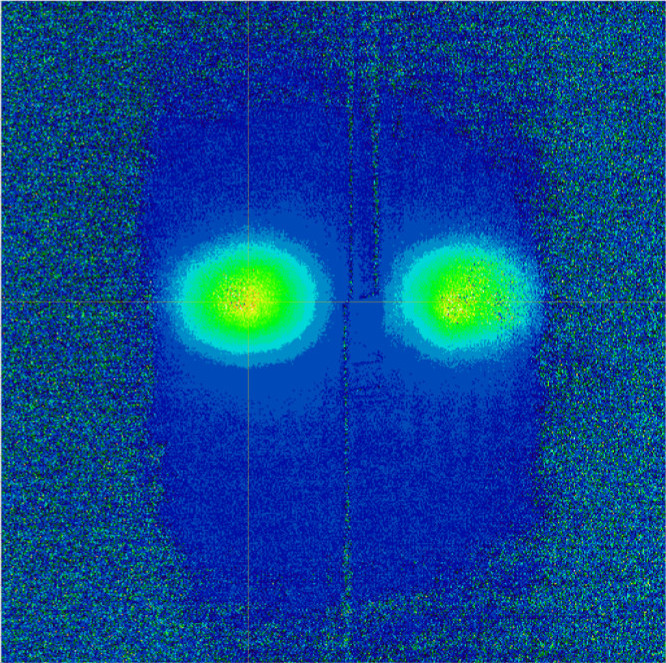
\includegraphics[width=0.35\linewidth]{figures/setup/coldatoms/log_abs_onlyPic}
\hspace{.15\linewidth}
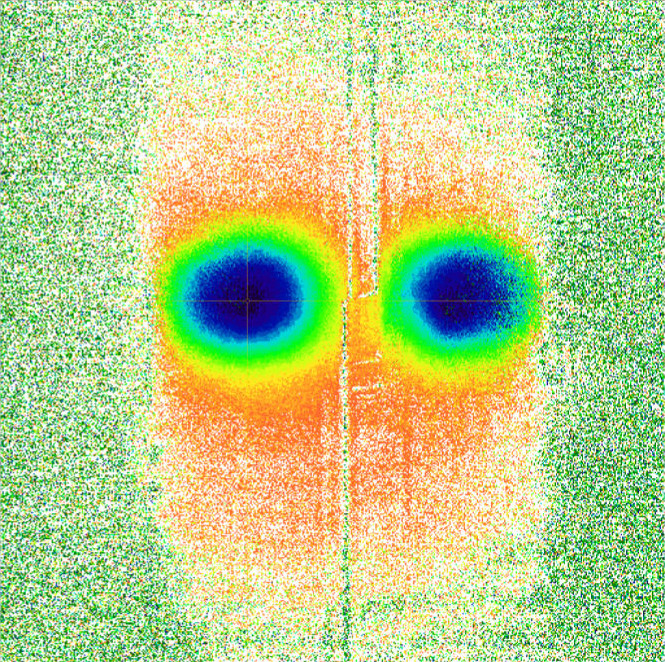
\includegraphics[width=0.35\linewidth]{figures/setup/coldatoms/nolog_abs_onlyPic}
\caption[Absorption \og no-log \fg{} ]{
Images du nuage atomique de mélasse optique par absorption du faisceau sonde côté.
\`A gauche, l'image est traitée par absorption selon l'équation \eqref{eq:Beer-Lambert_integ}.
\`A droite, l'image est traitée selon l'équation \eqref{eq:nolog_abs}.
Les graphes sous les images sont les profils de densité du nuage en coupe horizontale.
L'échelle de couleur est différente pour les deux images, adaptée à l'échelle des profils en coupe représentés.
Les zones bruitées à gauche et à droite ne sont pas éclairées par le faisceau sonde. 
En absorption \og no-log \fg{}, le bruit est plus important dans les zones sombres, mais réduit au centre et sur les bords du nuage.
%Le bruit y est beaucoup plus important si l'on ne prend pas le logarithme du signal (image de droite).
%Cependant, le bruit y est fortement réduit au centre du nuage.
}
\label{fig:nolog_abs}
\end{figure}	

%\clearpage
\subsubsection*{Estimation de la température}
\noindent L'imagerie par absorption permet facilement d'estimer la température du nuage atomique.
En effet, la distribution des impulsions dans le nuage suit la distribution de Maxwell-Boltzmann tant que celui-ci n'est pas condensé.
L'évolution de la taille gaussienne du nuage après extinction du piège, dictée par l'impulsion moyenne dans le nuage,  nous renseigne alors sur sa température par l'équation de propagation balistique
\begin{equation}
\label{eq:tempfit}
\Delta x^2 (t) = \Delta x^2(t_0) + \frac{\kb T}{m} \cdot (t-t_0)^2,
\end{equation}
où $\Delta x$ est l'extension spatiale du nuage dans la direction $x$, $t$ le temps et $t_0$ la référence de temps, $\kb$ la constante de Boltzmann, $m$ la masse d'un atome et $T$ la température du nuage.
En imageant le nuage à différents moments de son expansion (\og temps de vol \fg{}) et en ajustant la largeur gaussienne du profil à l'équation \eqref{eq:tempfit}, on accède à la fois à la température $T$ du nuage et à sa taille initiale dans le piège $\Delta x(t=0)$.
La figure \ref{fig:Tempfit} représente un ajustement de l'évolution de la taille du nuage après relâchement du piège.
%
\begin{figure}[!h]
\centering
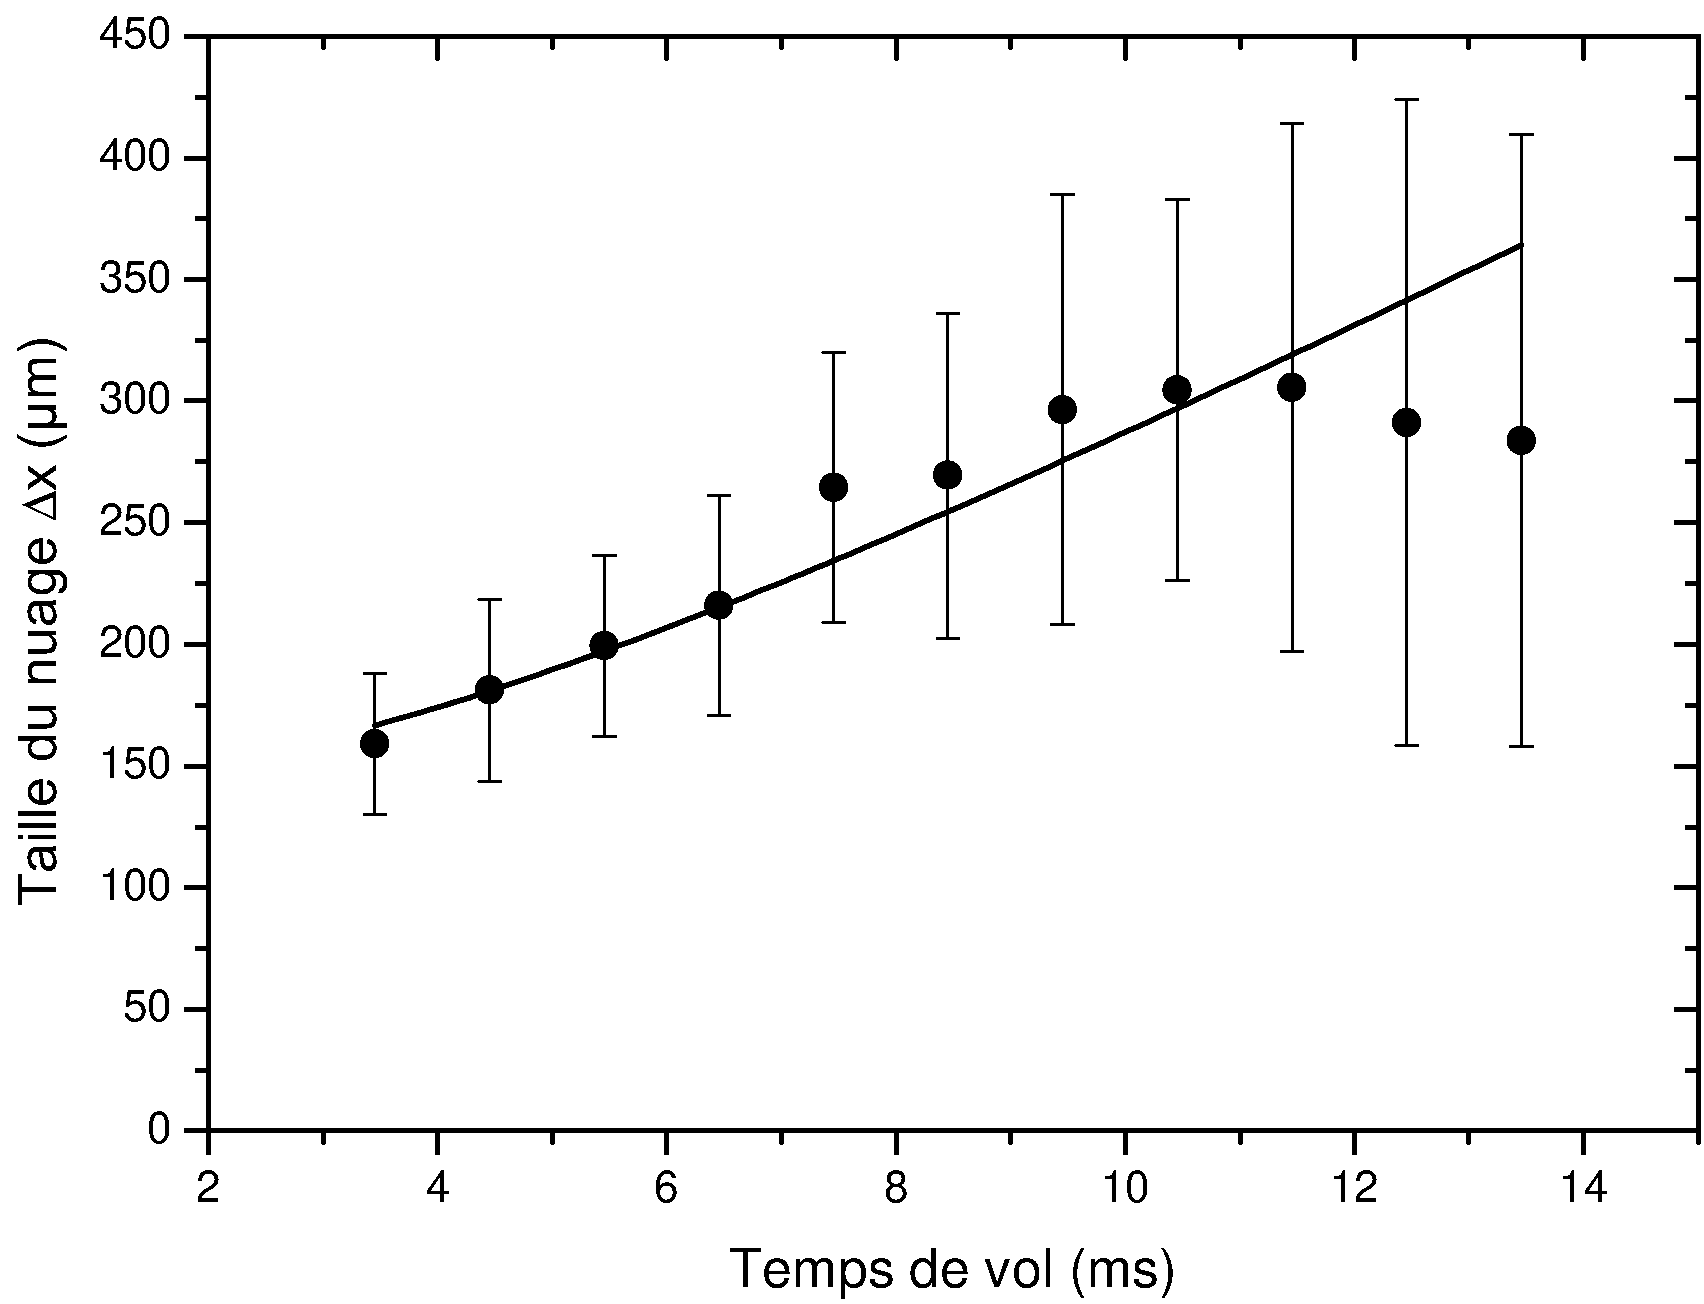
\includegraphics[width=.6\linewidth]{figures/setup/coldatoms/Tempfit}
%donnees du 1er sept 2017
\caption[Estimation de la température d'un nuage par temps de vol]{
Estimation de la température d'un nuage par temps de vol.
Le graphe représente l'évolution de la taille d'un nuage de mélasse optique, en fonction du temps écoulé depuis l'extinction des lasers.
L'ajustement selon l'équation \eqref{eq:tempfit} permet d'estimer la température du nuage à $\SI{6.43}{} \pm\SI{1}{\uK}$, et sa taille initiale à $\SI{142}{} \pm \SI{13}{\um}$.
}
\label{fig:Tempfit}
\end{figure}
	
\clearpage	
\subsection{Quelques nuages typiques}
\noindent Nous avons décrit ici les éléments de notre dispositif qui servent à produire et caractériser des nuages d'atomes ultra-froids.
Le tableau \ref{tab:nuages} présente les caractéristiques principales des différents types de nuages atomiques que nous utiliserons pour y exciter des atomes de Rydberg.

\begin{table}[h!]
	\centering
	\caption[Quelques nuages typiques]{Quelques nuages typiques de notre expérience.
	Pour chacun, nous donnons les caractéristiques suivantes : nombre d'atomes $N$, taille $\Delta x$ du nuage selon $x$, taille $\Delta y,z$ du nuage selon $y$ et $z$, température $T$ est distance à la puce $d$.
	}
	\label{tab:nuages}
	\begin{tabular}{c | c c c c c}
		\toprule\midrule
		{nuage}
		&N 
		&$\Delta x$
		&$\Delta y,z$
		&T
		&d
		\\
		\midrule
		QUAD-MOT
		&quelques \num{e8}
		&
		&
		&\SI{400}{\uK}
		&\SIrange{1}{3}{\mm}
		\\
%		U-MOT lointain
%		&
%		&
%		&
%		&idem
%		&idem
%		\\
		U-MOT proche
		&\SI{e7}
		&\SI{200}{\um}
		&\SI{200}{\um}
		&\SI{40}{\uK}
		&\SI{600}{\um}
		\\
		mélasse optique
		&\SI{5e6}
		&\SI{80}{\um}
		&\SI{80}{\um}
		&\SI{10}{\uK}
		&\SI{600}{\um}
		\\
		piège mag. chaud
		&\SI{1.5e6}
		&
		&
		&\SI{40}{\uK}
		&
		\\
		piège mag. froid
		&\SI{1.2e4}
		&\SI{45}{\um}
		&\SI{4.5}{\um}
		&\SI{0.75}{\uK}
		&\SI{450}{\um}
		\\
		BEC
		&\SIrange{8000}{20000}
		&
		&
		&\SIrange{30}{80}{\nano\K}
		&
		\\
		\midrule
		\bottomrule
 	\end{tabular}
\end{table}

\noindent Ces différents nuages d'atomes froids, ou ultra-froids, vont nous permettre d'explorer l'excitation d'atomes de Rydberg dans différentes conditions.

\clearpage
\section{Excitation et détection d'atomes de Rydberg près d'une puce}

\noindent Cette diversité de nuages atomiques nous permet d'exciter des atomes de Rydberg dans différentes conditions de densité atomique, de température et de distance à la puce.
Nous présentons dans le reste de ce chapitre la partie de notre dispositif expérimental servant à exciter, détecter et manipuler les atomes de Rydberg.
Notre dispositif est particulier dans la mesure où tout ce qui concerne les niveaux de Rydberg a lieu près d'une surface, la puce atomique.
Des champs parasites électriques parasites étant inévitables à proximité d'une surface, la grande sensibilité électromagnétique des atomes de Rydberg sera mise à rude épreuve.

Après avoir donné le principe de l'excitation à deux photons des niveaux de Rydberg et de la détection par ionisation sélective, nous ferons une présentation de rapide de l'effet Stark et de ses conséquences sur nos expériences.
Nous décrirons ensuite les techniques mises en place afin de contrôler les champs électriques près de la puce.
Nous finirons ce chapitre par une présentation de la technique de spectroscopie microonde des niveaux de Rydberg et de son utilisation pour mesurer les champs électriques résiduels.

%\clearpage
\subsection{L'excitation à deux photons des atomes de Rydberg}\label{subsec:2photon_excite}
\noindent Les atomes de rubidium piégés dans un nuage près de la puce sont excités vers les niveaux de Rydberg par une transition laser à deux photons désaccordée par rapport au niveau intermédiaire.
Dans nos expériences, deux niveaux de Rydberg différents ont été excités par laser à partir de l'état fondamental 5S$_{1/2}$ : le niveau 60S$_{1/2}$ et le niveau 50D$_{3/2}$.
Nous décrivons ici l'excitation d'un nuage d'atomes de Rydberg au sein d'un nuage froid dans le piège magnétique, en négligeant les interactions entre atomes de Rydberg et en nous concentrant sur le niveau $\mathrm{60S_{1/2}}$.

La transition du niveau fondamental au niveau de Rydberg est faite par l'absorption d'un photon rouge à $\lambda = \SI{780}{\nano\meter}$, désaccordé de $\delta=+2\pi\times\SI{540}{\MHz}$ par rapport à la transition $\mathrm{5S_{1/2},F=2 \rightarrow 5P_{3/2},F'=3}$, et d'un photon bleu à $\lambda = \SI{480}{\nano\meter}$, accordé pour satisfaire la condition de résonance vers le niveau choisi.
La figure \eqref{fig:2photons} représente le schéma de niveaux de l'excitation du niveau $\mathrm{60S_{1/2}}$.
Les deux faisceaux d'excitation sont superposés et se propagent selon la direction $+x$. Leurs polarisations sont définies par rapport à l'axe de quantification des niveaux atomiques, déterminé par le champ magnétique de biais $B_x$ dans le fond du piège.
La figure \eqref{fig:lasers_excit} représente la géométrie des faisceaux laser d'excitation.
Dans cette configuration, seul le sous-niveau $m_j=+1/2$ du niveau 60S est excité.
%
\begin{figure}[!h]
\centering
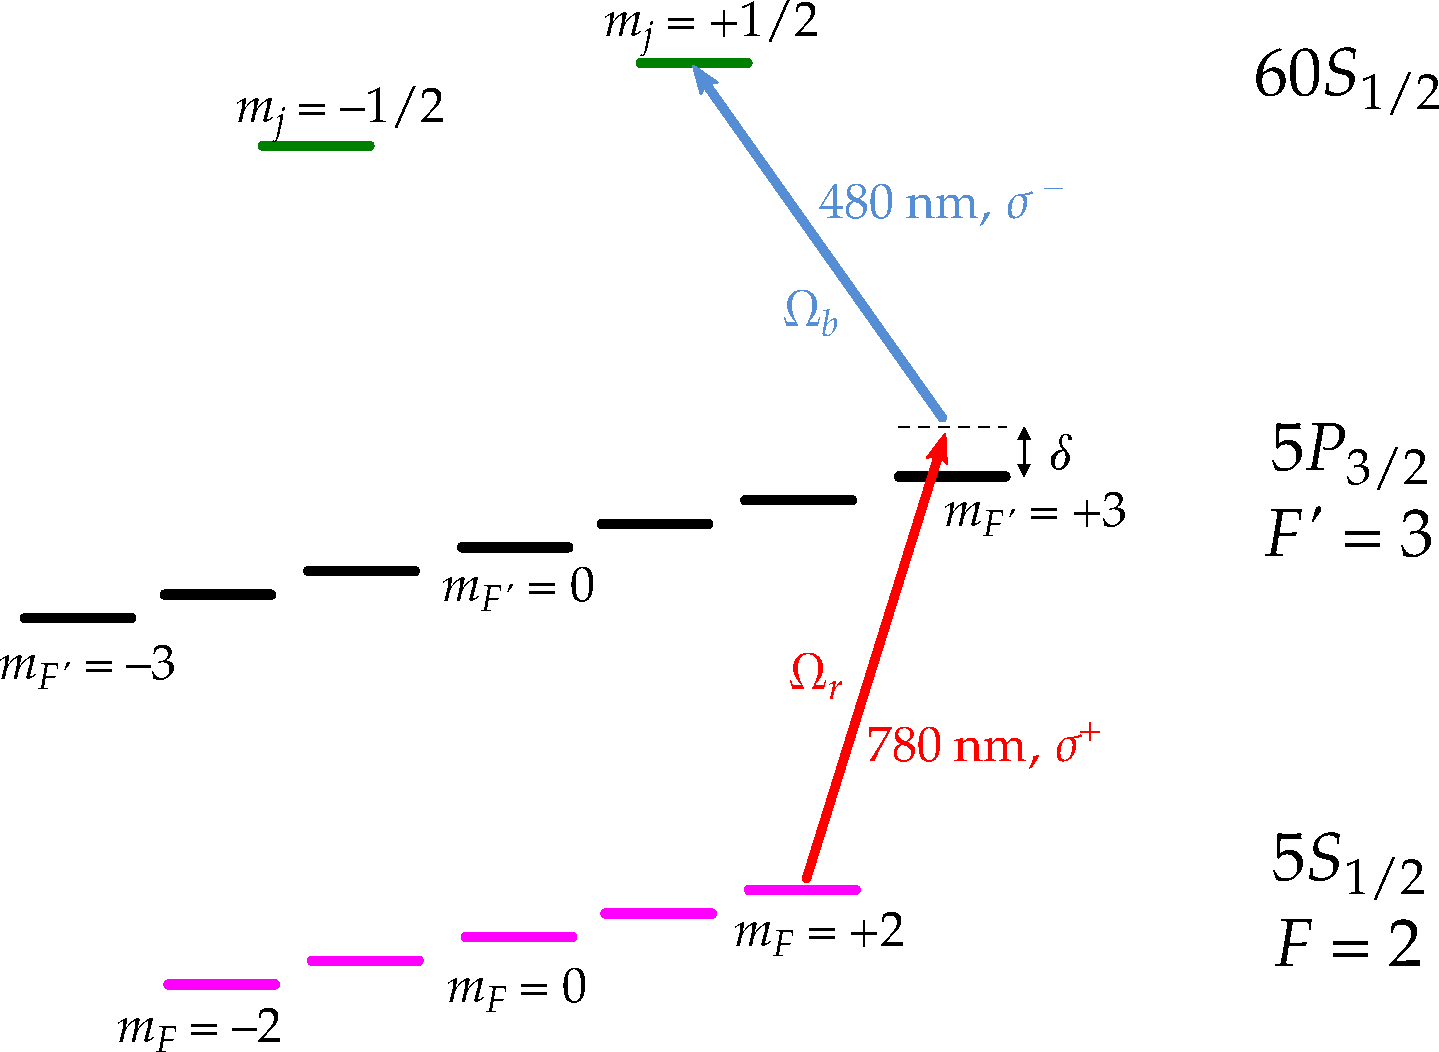
\includegraphics[width=.7\linewidth]{figures/setup/rydberg/2photons}
\caption[Excitation du niveau 60S]{Schéma de l'excitation laser du niveau 60S, à partir d'atomes de \Rb{87} dans le niveau fondamental dans le piège magnétique.
La polarisation de chaque laser est indiquée.
$\Omega_r$ et $\Omega_b$ sont les fréquences de Rabi des transitions à \num{780} et \SI{480}{\nano\meter} respectivement.
$\delta=+2\pi\times\SI{540}{\MHz}$ est le désaccord par rapport au niveau intermédiaire.
}
\label{fig:2photons}
\end{figure}

Le laser rouge d'excitation est extrait du laser maître, mentionné en \ref{subsec:exp_seq}, puis décalé en fréquence par un modulateur acousto-optique.
Le laser bleu à $\SI{480}{\nm}$ est généré par un système commercial TOPTICA TA-SHG 110 de diode laser amplifiée puis doublée en fréquence.
La lumière laser à $\SI{960}{\nm}$ est asservie en fréquence à la même cavité de Fabry-Pérot que le laser maître.
Un modulateur acousto-optique intervient entre la diode et la cavité Fabry-Pérot, qui nous permet de contrôler la fréquence de la diode sur une plage d'environ $\SI{75}{\MHz}$.
%Le laser à $\SI{960}{\nm}$ est ensuite amplifié puis doublé en fréquence grâce à un cristal non-linéaire placé dans une cavité.
Après doublage de la fréquence, cela correspond à un balayage de la fréquence du laser bleu sur une plage de $\SI{150}{\MHz}$.
Le système de stabilisation et de distribution des faisceaux laser d'excitation des niveaux de Rydberg est détaillé en annexe \ref{app:laserlock}.

Le faisceau rouge a typiquement un col de $\SI{150}{\um}$ et une puissance de $\SI{50}{\micro\watt}$ au niveau des atomes.
Le laser rouge est désaccordé de $\delta=+\SI{540}{\MHz}$ par rapport à la transition $ \ket{\mathrm{5S_{1/2},F=2,m_F=+2}} \rightarrow \ket{\mathrm{5P_{3/2},F'=3,m_F'=+3}}$, dont le moment de transition dipolaire vaut $\SI{2.98931 (62)} ea_0$ \cite{DATA_STECKRB87}.
D'après les caractéristiques du faisceau, la fréquence de Rabi correspondant à cette transition est de l'ordre de $\Omega_r \simeq 2\pi\times \SI{40}{\MHz}$.
Le taux d'émission spontanée de photons rouge par le niveau intermédiaire, de durée de vie $\Gamma^{-1} \simeq \SI{26}{\ns}$, est donné par
\begin{equation}
\label{eq:scattering_5P3/2}
\Gamma_{sp} = \frac{1}{2} \frac{\Omega_r^2 \Gamma}{\delta^2 + \Omega_r^2 + \Gamma^2}
\simeq \frac{\Omega_r^2}{2\delta^2} \Gamma,
\end{equation}
où $\Gamma = 2\pi \times \SI{6.065}{\MHz}$ est la largeur naturelle du niveau $\mathrm{5P_{3/2}}$.
La dernière égalité est vérifiée dans l'approximation $\delta^2 \gg \Omega_r^2, \Gamma^2$, qui est ici valide.
Avec nos valeurs d'intensité et de désaccord du laser, on obtient $\Gamma_{sp} \simeq \num{2.74e-3} \Gamma = 2\pi\times \SI{0.0166}{\MHz}$, ce qui correspond à l'émission d'un photon  toutes les $\Gamma_{sp}^{-1} = \SI{9.565}{\us}$.
Or lorsqu'un atome absorbe et ré-émet un tel photon, il gagne une énergie moyenne
$\Delta E = p^2/(2m_{Rb87}) = h^2/(2m_{Rb87} \lambda^2) = \frac{3}{2}\kb\times\SI{120}{\nano\kelvin}$.
Étant données nos valeurs d'intensité et de désaccord, cela implique un taux de chauffage de $\Gamma_{sp}\,\Delta E /\kb = \SI{12.6}{\nano\K/\us}$.
Le piège est ainsi chauffé par le laser rouge d'excitation, %\footnote{
%Le problème du chauffage du nuage est discuté plus en détail en \ref{subsec:rate_equation}.}
ce qui limite à la fois la puissance que l'on peut envoyer sur le nuage, et le nombre d'impulsions laser d'excitation que l'on peut faire subir à un même nuage sans l'altérer.

Le faisceau bleu a typiquement un col de $\SI{22}{\um}$ et une puissance estimée à $\SI{4}{\milli\watt}$ au niveau des atomes.
Le moment dipolaire de la transition $ \ket{\mathrm{5P_{3/2},F'=3,m_F'=+3}} \rightarrow \ket{\mathrm{60S_{1/2},m_j=+1/2}}$ est cependant bien plus faible que le précédent, et vaut $\SI{9.9e-3} ea_0$
\footnote{Nous rappelons ici que, comme nous l'avons mentionné en \ref{sec:alkalRydberg}, le bon nombre quantique magnétique pour les niveaux de Rydberg est $m_j$ et non pas $m_F$.}.
La fréquence de Rabi pour cette transition est alors de $\Omega_b = 2\pi\times \SI{8}{\MHz}$.
Les fréquences de Rabi des deux transitions satisfont l'approximation $\Omega_{r,b} \ll \delta$, ce qui nous permet de négliger l'occupation du niveau intermédiaire, et donc de l'éliminer adiabatiquement \cite{TXT_ASPECTFABRE_QUANTOPT}.
Le système à trois niveaux se ramène alors à un système effectif à deux niveaux, couplés par une fréquence de Rabi
\begin{equation}
\label{eq:Rabi_2photons}
\Omega = \frac{\Omega_r \Omega_b}{\delta}.
\end{equation}
Avec nos paramètres, on obtient une fréquence de Rabi $\Omega = 2\pi \times \SI{296}{\kHz}$ pour la transition $\ket{\mathrm{5S_{1/2},F=2,m_F=+2}} \rightarrow \ket{\mathrm{60S_{1/2},m_j=+1/2}}$.
Ce paramètre peut être varié simplement en ajustant la puissance du laser rouge ou la puissance du laser bleu.

%
\begin{figure}[!h]
\centering
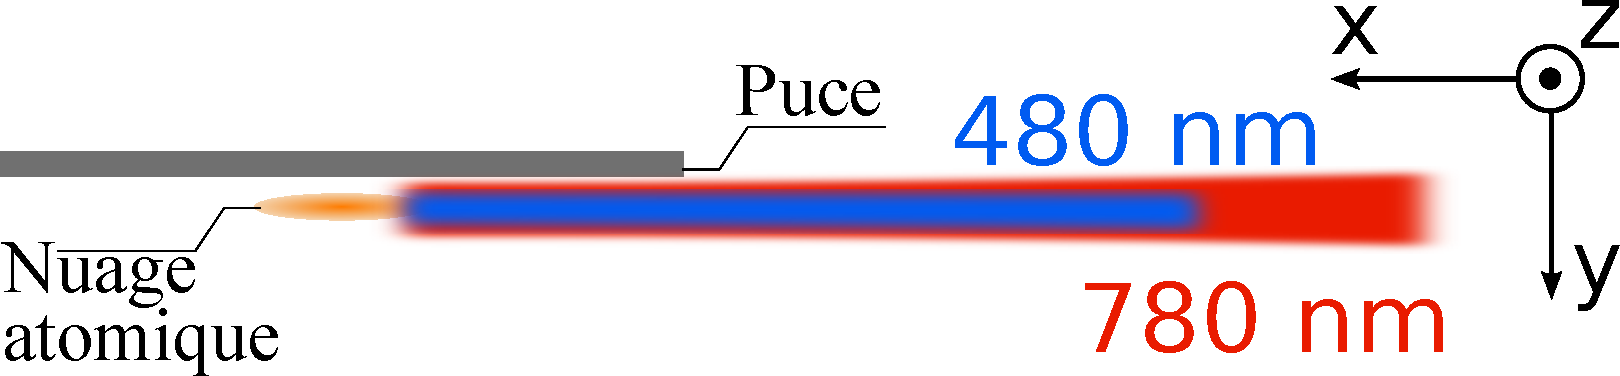
\includegraphics[width=.6\linewidth]{figures/setup/rydberg/lasers_excit}
\caption[Faisceaux laser pour l'excitation des Rydberg]{Schéma représentant la géométrie des faisceaux laser d'excitation.
}
\label{fig:lasers_excit}
\end{figure}

%\clearpage	
\subsection{La détection par ionisation des atomes de Rydberg}\label{subsec:detection}
\noindent L'électron de valence d'un atome de Rydberg alcalin est très proche du seuil d'ionisation.
Il est donc très facile de l'arracher au noyau en appliquant un champ électrique.
Nous exploitons cette caractéristique pour détecter les atomes de Rydberg par ionisation en champ électrique :
une fois l'atome ionisé, le c\oe ur atomique est accéléré par des électrodes vers un détecteur à avalanche (Channeltron).


%
\begin{figure}[h]
\centering
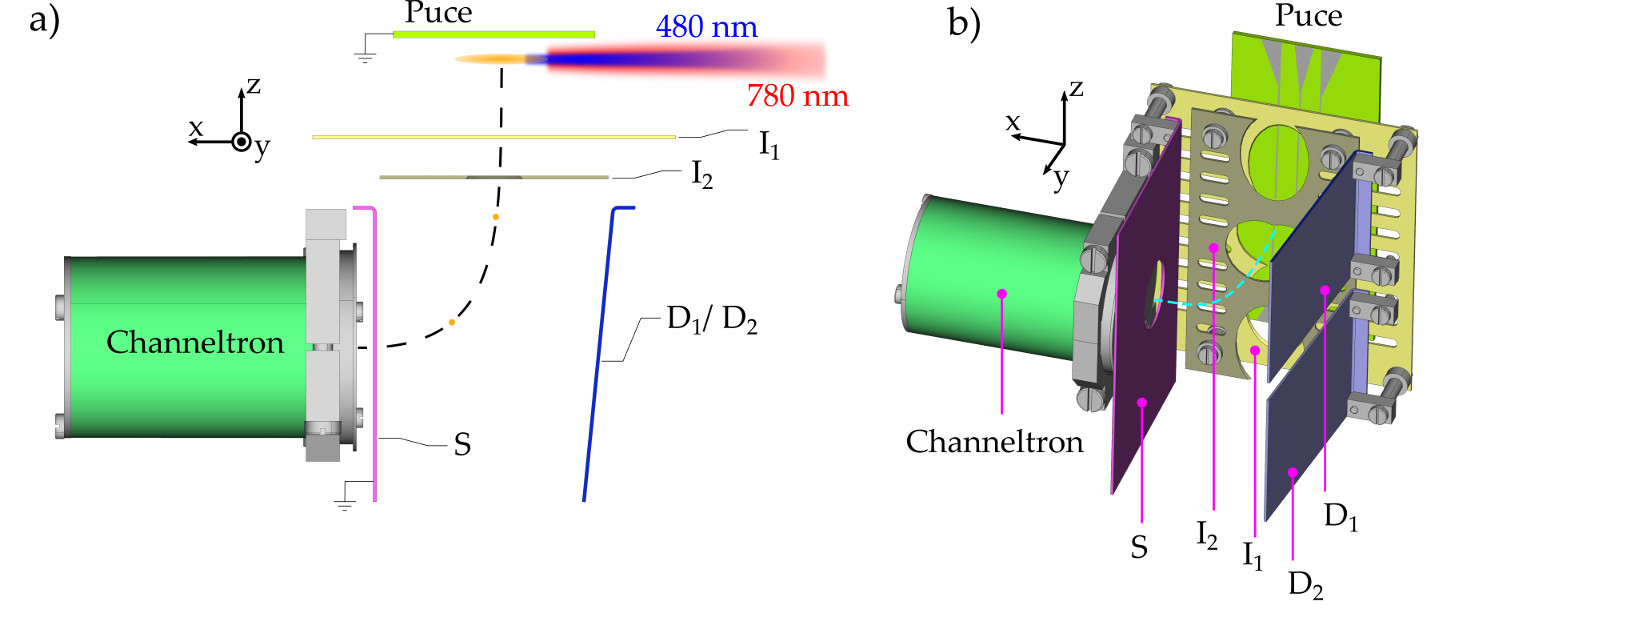
\includegraphics[width=\linewidth]{figures/setup/rydberg/schema_detect}
\caption[Système de détection des atomes de Rydberg]{Schéma représentant le système de détection des atomes de Rydberg.
\textbf{a)} vu de dessus et \textbf{b)} en projection axonométrique.
Après excitation, les atomes de Rydberg sont ionisés par les élctrodes $I_1$ et $I_2$.
Les ions ainsi créés et accélérés sont défléchis par les électrodes $D_1$ et $D_2$, en direction du détecteur Channeltron.
L'électrode $S$ est mise à la masse et sert à écranter la tension présente à l'entrée du Channeltron.
La trajectoire des ions est indiquée en lignes pointillées et les faisceaux lasers d'excitation sont représentés en \textbf{a)}.
}
\label{fig:schema_detect}
\end{figure}
%
La figure \eqref{fig:schema_detect} présente un schéma détaillé du système de détection par ionisation.
Au moment de la détection, une tension négative est appliquée sur les électrodes d'ionisation $I_1$ et $I_2$.
La tension sur ces électrodes crée un champ électrique de l'ordre de quelques $\SI{100}{\V/\cm}$ au niveau des atomes, la puce étant mise à la masse.
Ce champ électrique ionise les atomes de Rydberg et accélère les ions positifs ainsi créés.
Ces ions sont ensuite défléchis en direction du Channeltron par les électrodes $D_1$ et $D_2$, mises en permanence à un potentiel $V_{defl} = +\SI{150}{\V}$.
Une grille placée à l'entrée du Channeltron est alimentée par une tension de $\SI{-3000}{\V}$.
Une électrode trouée mise à la masse est placée devant cette grille afin d'écranter les $\SI{-3000}{\V}$ pour la région de piégeage des atomes.
Lorsque les ions arrivent dans le Channeltron, celui-ci génère par avalanche un signal électronique qui est envoyé vers un amplificateur et un discriminateur permettant de décompter les ions détectés.
Le Channeltron est isolé thermiquement et chauffé à une température de $\SI{42}{\K}$ afin d'augmenter son efficacité.

\newpage
\subsubsection*{Sélectivité de niveau de la détection par ionisation}
\noindent Chaque atome de Rydberg présente une énergie différente, telle que discutée en \ref{sec:alkalRydberg}.
Cela signifie qu'ils sont tous à une distance différente du seuil d'ionisation, et \textit{in fine} que chaque niveau de Rydberg sera ionisé pour une valeur de champ électrique spécifique.
On peut ainsi appliquer une rampe de tension sur les électrodes d'ionisation, afin que chaque niveau de Rydberg soit ionisé à un instant différent.
Alors, les ions correspondants seront détectés à des instants différents par le Channeltron et pourront être distingués.
Des fenêtres temporelles de détection peuvent alors être définies, qui permettent de compter les atomes détectés dans chacun des différents niveaux.
La figure \eqref{fig:arrTimes6057} montre un signal de détection sélective des niveaux de Rydberg $\mathrm{60S_{1/2}}$ et $\mathrm{57S_{1/2}}$.
La rampe de tension et les fenêtres temporelles de détection sont optimisées afin de distinguer au mieux les différents niveaux de Rydberg détectés.
L'efficacité de détection de notre dispositif a été mesurée à $\SI{90}{} \pm \SI{10}{\percent}$, en comparant le nombre d'atomes de Rydberg détectés par ionisation à la réduction du nombre d'atomes dans l'état fondamental mesuré par absorption \cite{PHD_CELISTRINO}.
%
\begin{figure}[!h]
\centering
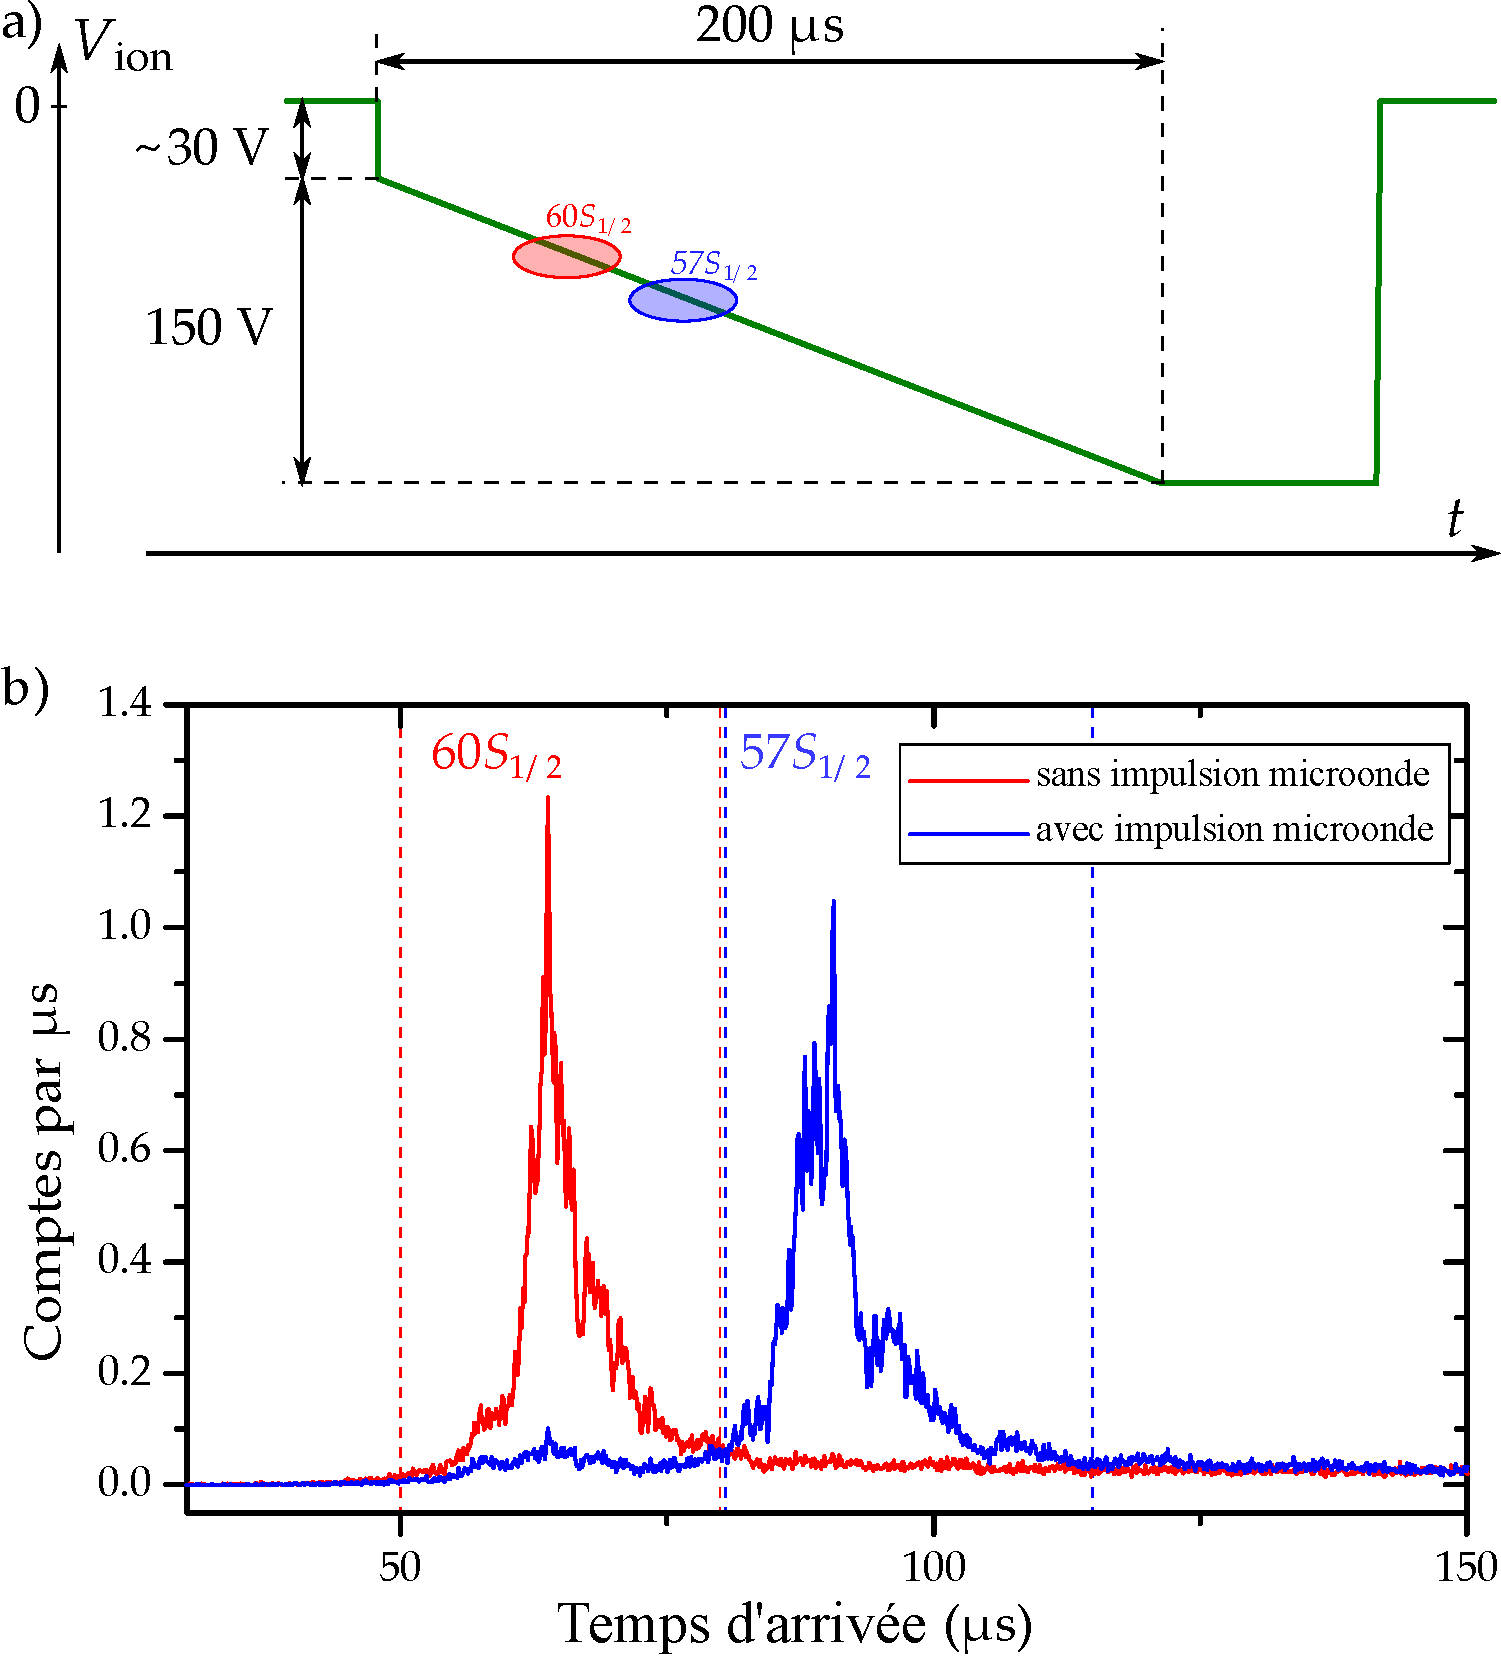
\includegraphics[width=.7\linewidth]{figures/setup/rydberg/arrTimes6057}
\caption[Détection sélective des niveaux $\mathrm{60S_{1/2}}$ et $\mathrm{57S_{1/2}}$]{
Détection sélective des atomes de Rydberg.
\textbf{a)} Une rampe de tension $V_{ion}$ typique appliquée sur les électrodes d'ionisation.
Les seuils d'ionisation des niveaux $\mathrm{60S_{1/2}}$ et $\mathrm{57S_{1/2}}$ sont indiqués en rouge et bleu respectivement.
\textbf{b)} Temps d'arrivée des ions correspondants. Des fenêtres temporelles de détection, représentées en pointillés, sont définies pour compter sélectivement les atomes dans les niveaux $\mathrm{60S_{1/2}}$ et $\mathrm{57S_{1/2}}$.
Les atomes sont préparés dans l'état $\mathrm{60S_{1/2}}$ et le niveau $\mathrm{57S_{1/2}}$ est peuplé par une impulsion $\pi$ de la transition microonde adéquate.
Les échelles de temps sont différentes en \textbf{a)} et \textbf{b)}.
}
\label{fig:arrTimes6057}
\end{figure}
%


\newpage		
\subsection{Les champs électriques parasites, défi des atomes de Rydberg sur puce}\label{subsec:flashRb}
	%problème des champs électriques et flash de Rb}
\noindent Comme nous l'avons dit au chapitre \ref{chapter:Rydberg}, les atomes de Rydberg sont des objets extrêmement sensibles au champ électromagnétique.
Or, dans notre expérience, nous souhaitons exciter et manipuler des atomes de Rydberg à proximité immédiate d'une surface, la puce à atomes.
Les champs électriques parasites étant inévitables près d'une surface, la présence de la puce va rendre difficile l'excitation et la manipulation des atomes de Rydberg.

\subsubsection*{Premiers spectres}
\noindent Ce problème est très clair sur les premiers spectres optiques que nous avons fait de la transition $\ket{\mathrm{5S_{1/2}}} \rightarrow \ket{\mathrm{60S_{1/2}}}$, présentés en figure \eqref{fig:vieilles_raies}.
%
\begin{figure}[!h]
\centering
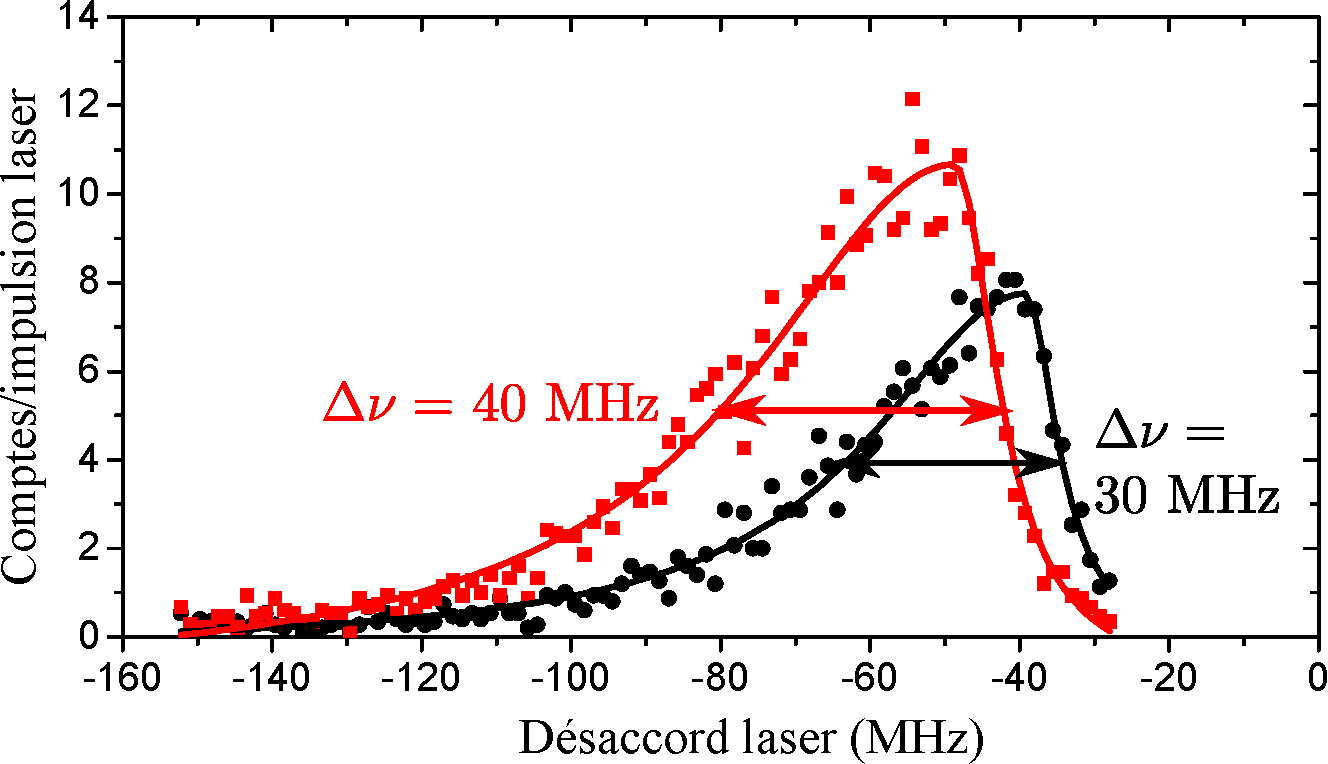
\includegraphics[width=.8\linewidth]{figures/setup/rydberg/vieilles_raies}
\caption[Spectres d'excitation laser 5S-60S avant le dépôt de rubidium sur la puce]{
Deux spectres laser de la transition $5\mathrm{S}\rightarrow60\mathrm{S}$, avant correction des inhomogénéités et de la dérive du champ électrique.
Leurs largeurs sont de $\SI{30}{\MHz}$ et $\SI{40}{\MHz}$ respectivement, et ils sont décalés en fréquence de $\SI{12}{\MHz}$ l'un par rapport à l'autre.
Les deux spectres ont été pris dans les mêmes conditions, à \SI{1}{\hour} d'intervalle, pendant laquelle un MOT était piégé devant la puce.
L'origine de l'axe des abscisses correspond à la fréquence résonante de la transition $\mathrm{5S}\rightarrow\mathrm{60S}$ en l'absence de champ électrique.
}
\label{fig:vieilles_raies}
\end{figure}
%
Ces premiers spectres présentent des largeurs de raie de plusieurs dizaines de $\si{\MHz}$, et une forme asymétrique caractéristique d'un élargissement Stark inhomogène.
De plus, une heure de fonctionnement de l'expérience cause un déplacement en fréquence de la raie de \SI{12}{\MHz}.

Cet effet est causé par la variation spatiale et temporelle du champ électrique dans la région du nuage atomique :
%L'énergie des niveaux de Rydberg dépend fortement du champ électrique extérieur au niveau de chaque atome.Ainsi, 
si les atomes dans différentes régions du nuage voient des champs électriques différents, la fréquence de la transition $\mathrm{5S}\rightarrow\mathrm{60S}$ sera déplacée différemment dans chaque région par l'effet Stark, et la raie spectrale s'en trouvera élargie.
Une largeur de raie de $\SI{40}{\MHz}$ correspond à un champ électrique variant de $\SIrange{0}{0.667}{\V/\cm}$ sur l'extension du nuage, d'après les coefficients Stark donnés en table \ref{tab:Stark_60S}.
Or le nuage utilisé pour ces spectres était un MOT de $\sim \SI{200}{\um}$ de diamètre, ce qui nous donne une valeur de gradient de champ électrique de l'ordre de $\SI{35}{(\V/\cm)\per\cm}$.


%\clearpage
\subsubsection*{Potentiel de contact du rubidium sur l'or et dépôt contrôlé}
\noindent La cause principale de l'inhomogénéité spatiale et temporelle des champs électriques est l'accumulation d'un dépôt d'atomes de rubidium sur la surface en or de la puce :
lorsque les atomes du piège sont relâchés à la fin de chaque séquence, une partie d'entre eux entre en contact avec la surface froide de la puce et s'y dépose.
Des dépôts volontaires d'atomes sur la puce, à partir de nuages piégés, nous ont confirmé l'importance de ce phénomène et de ses effets sur les spectres d'excitation laser.

L'accumulation d'atomes de rubidium sur la puce forme d'importants dipôles électriques.
En effet, les niveaux de Fermi de l'or et du rubidium étant différents, lorsque les deux métaux sont mis en contact les électrons se déplacent de l'un à l'autre pour équilibrer les niveaux de Fermi.
Un potentiel électrostatique de contact est alors créé entre l'or et le rubidium.
La surface de la puce étant mise à la masse, ce sont les plaques de rubidium déposé qui se chargent à $\SI{2.5}{\V}$ environ.
Or le dépôt de rubidium depuis les nuages piégés est un processus lent et non contrôlé, sur des échelles de longueur de l'ordre du $\si{\mm}$.
Cela a pour conséquence un champ électrique variant dans le temps et inhomogène à une distance de la puce inférieure à quelques $\si{\mm}$.
C'est justement là que se trouvent les atomes piégés que l'on souhaite exciter.

La solution que nous avons mise en \oe uvre fut de saturer le dépôt de rubidium sur la puce, en faisant un dépôt contrôlé macroscopique sur une surface grande devant la région de piégeage.
Pour que cela fonctionne, il est important que le rubidium déposé reste métallique, non oxydé, et ne migre pas dans le cryostat en raison de différences de températures.
Ces contraintes nous ont décidés à faire le dépôt de rubidium à froid, lorsque le cryostat est sous vide et thermiquement stable.
Le dépôt contrôlé a été réalisé grâce à l'installation de dispenseurs de rubidium dans le cryostat, orientés de façon à pouvoir couvrir la puce de rubidium métallique.
La figure \eqref{fig:depotRb} illustre qualitativement la structure des champs électriques au voisinage de la puce avant et après le dépôt de rubidium.
Les dispenseurs nous ont permis de déposer une couche de rubidium, estimée à environ $\SI{80}{\nano\meter}$ d'épaisseur, sur une partie importante de la surface de la puce.

%
\begin{figure}[h]
\centering
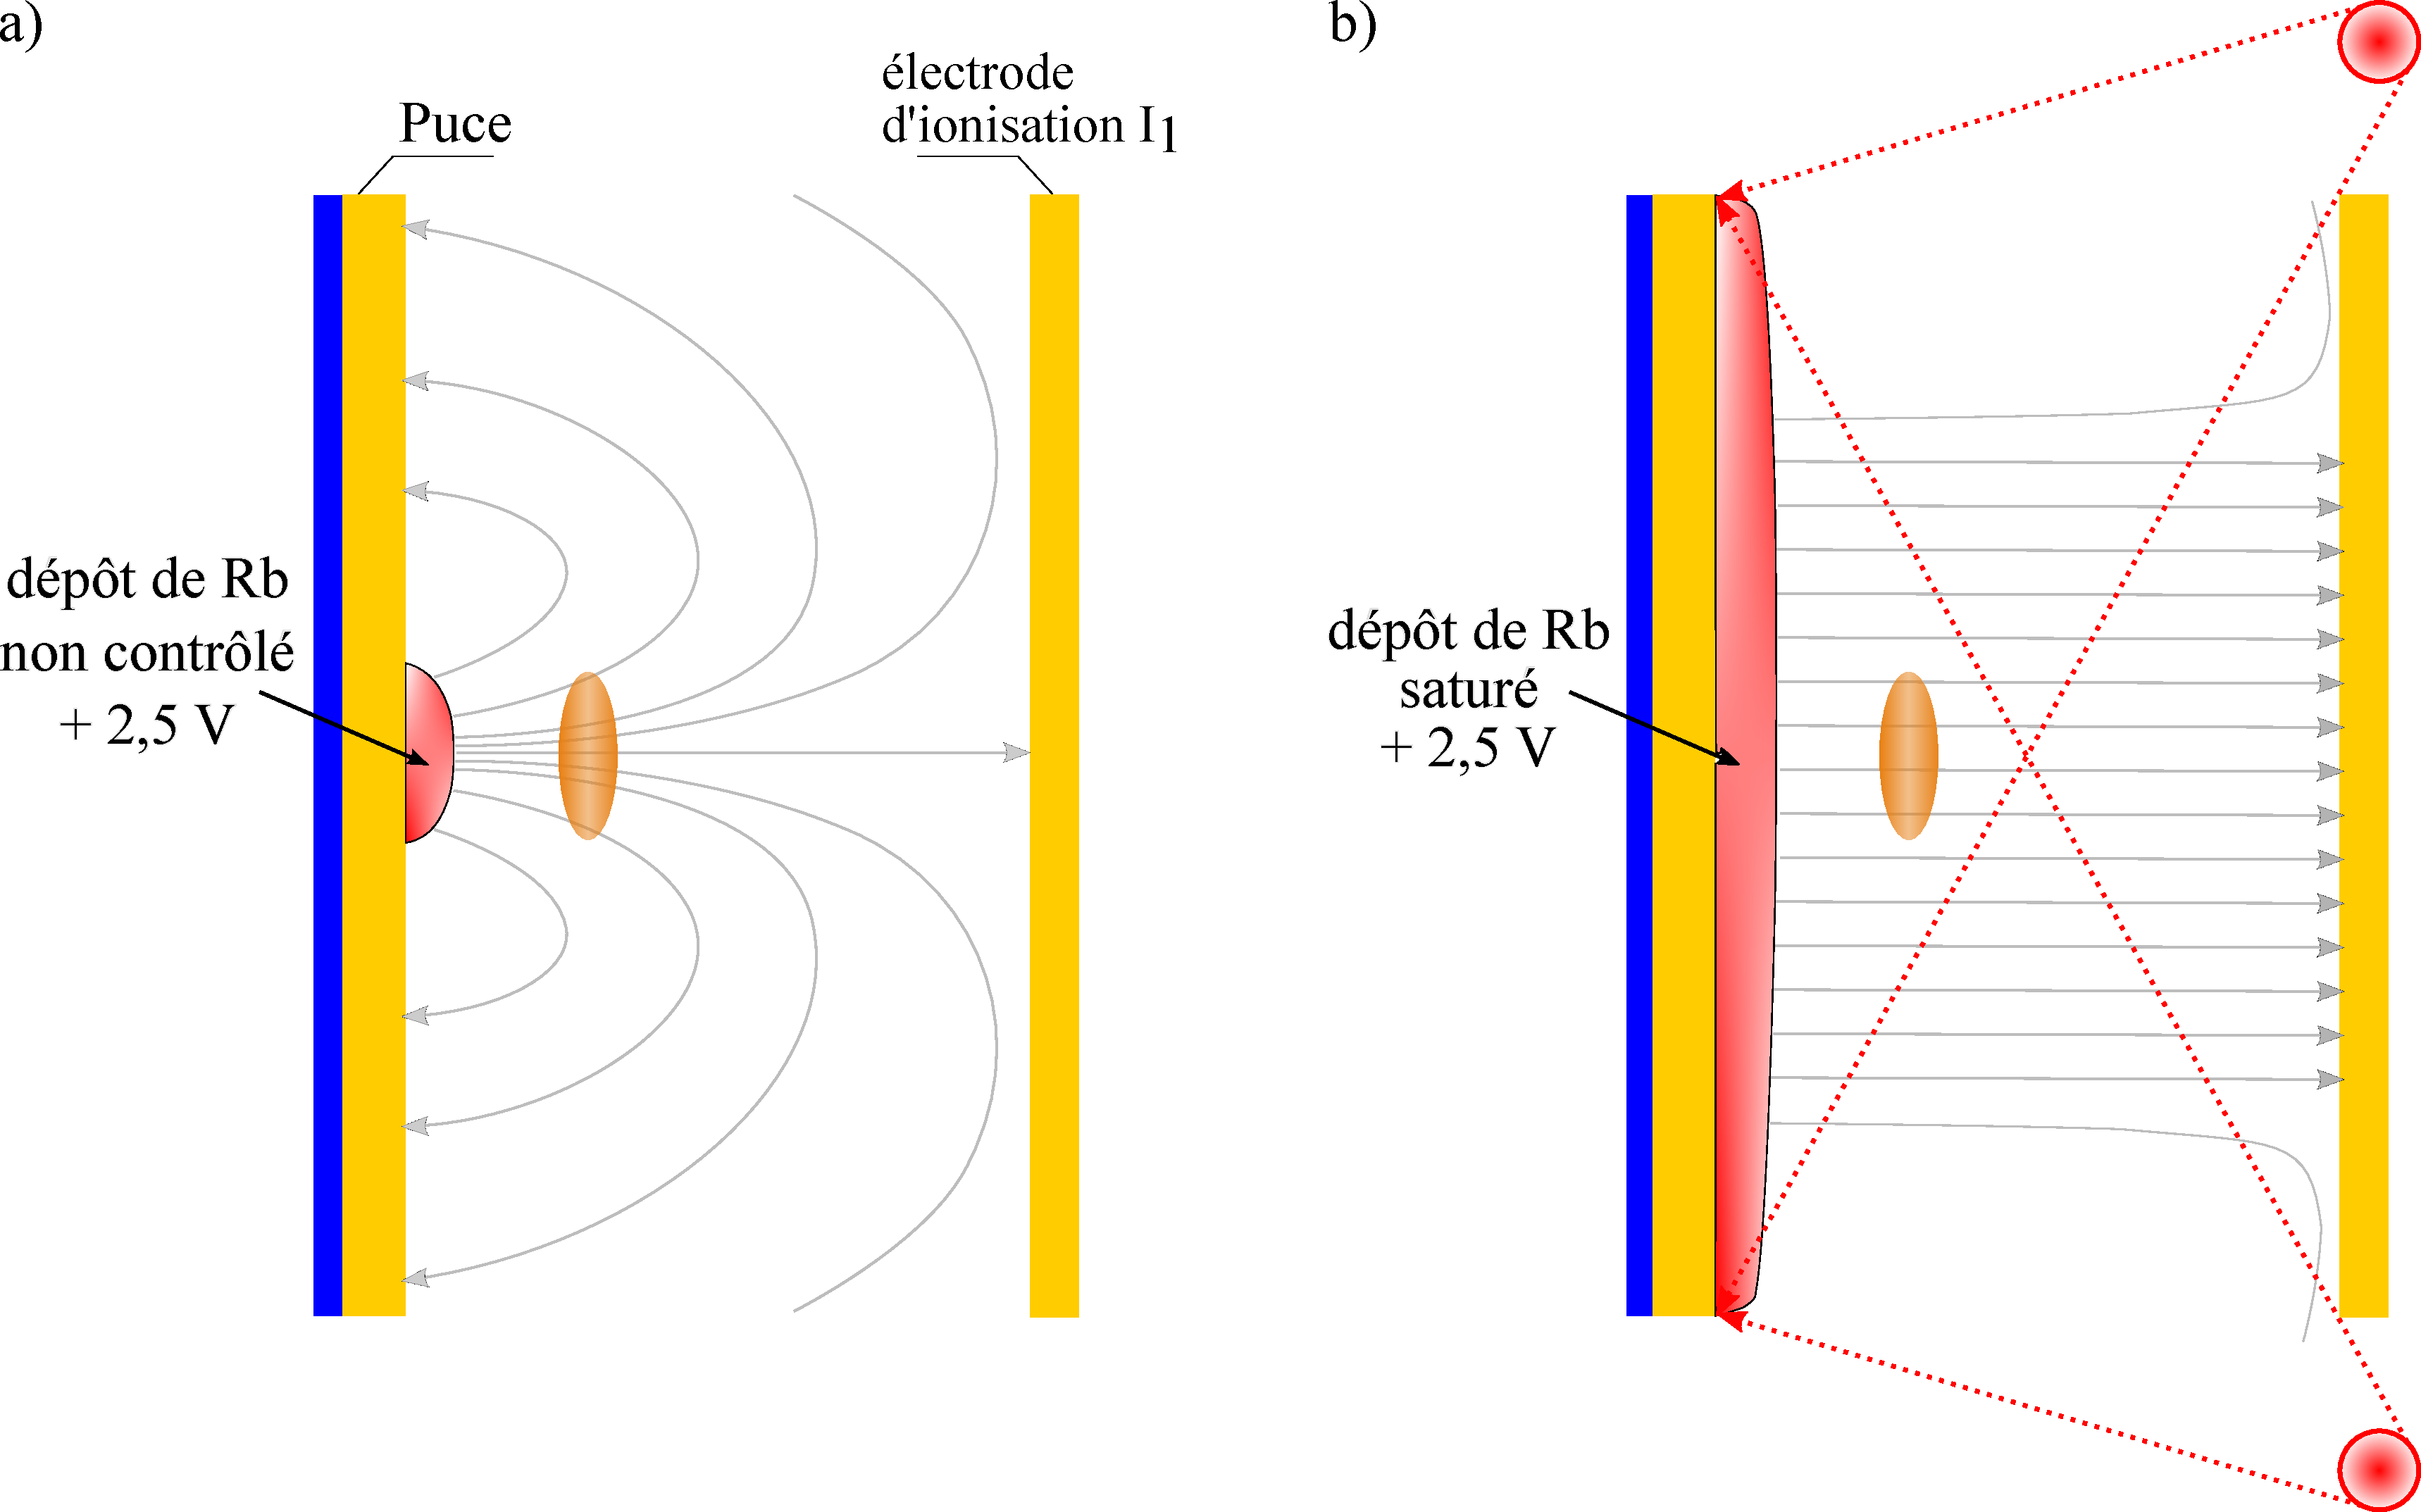
\includegraphics[width=\linewidth]{figures/setup/rydberg/depotRb}
\caption[Dépôt contrôlé de rubidium sur la puce]{
Schéma illustrant les dépôts de rubidium sur la puce et les champs électriques qui en résultent.
Les dépôts de rubidium sont représentés en rouge et les traits gris fléchés représentent les lignes de champ électrique.
Les surfaces représentées en jaune (puce et électrode d'ionisation) sont mise à la masse.
L'ovale orange représente la position du nuage atomique (les échelles ne sont pas respéctées).
\textbf{a)} Dépôt non-contrôlé dû aux atomes piégés : le champ électrique est inhomogène et varie dans le temps.
\textbf{b)} Dépôt contrôlé réalisé grâce aux dispenseurs de rubidium (indiqués par les cercles rouges) : le champ électrique créé par le potentiel de contact rubidium-or est homogène et stable dans le temps.
}
\label{fig:depotRb}
\end{figure}
%

\clearpage
Un spectre d'excitation laser enregistré juste après ce dépôt de rubidium dans un MOT à $\SI{500}{\um}$ de la puce est présenté en figure \eqref{fig:raiefine_depot}.
Les conditions d'excitation sont similaires à celles des spectres présentés en figure \eqref{fig:vieilles_raies}, mais la largeur de raie spectrale est de seulement $\Delta\nu=\SI{1.7}{\MHz}$.
Le dépôt de rubidium a donc eu un effet extrêmement bénéfique sur l'excitation d'atomes de Rydberg au voisinage de la puce.

Des optimisations ultérieures des conditions d'excitation nous ont permis d'obtenir des raies spectrales d'une largeur de $\Delta\nu \simeq \SI{625}{\kHz}$, que nous attribuons majoritairement à une fluctuation lente de la fréquence des lasers \cite{PHD_CELISTRINO}.

\begin{figure}[h]
\centering
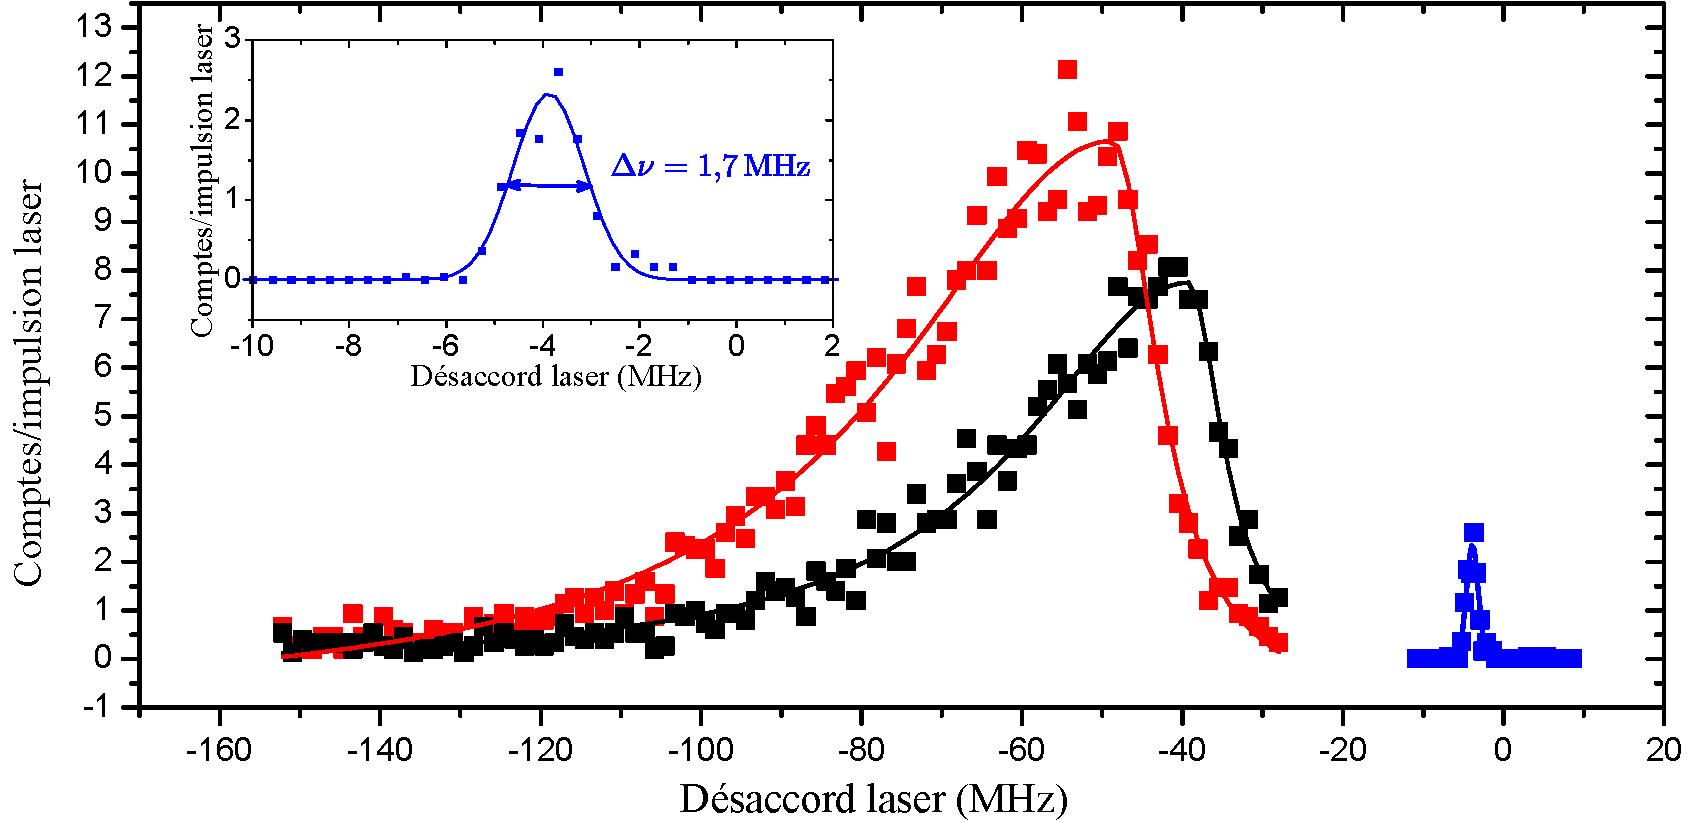
\includegraphics[width=\linewidth]{figures/setup/rydberg/avant-apres-coating}
%setup/rydberg/raiefine_depot}
\caption[Spectres d'excitations laser 5S-60S avant et après le dépôt de rubidium sur la puce]{
Spectres d'excitations laser 5S-60S d'atomes piégés dans un MOT, juste avant (noir et rouge) et juste après (bleu) le dépôt de rubidium sur la puce.
L'insert reprend le spectre bleu à une échelle plus adaptée.
L'ajustement gaussien donne une largeur de $\Delta\nu=\SI{1.7}{MHz}$ :
la largeur de raie a été considérablement réduite par le dépôt contrôlé de rubidium.
}
\label{fig:raiefine_depot}
\end{figure}


%\clearpage	
\subsection{Contrôle du champ électrique perpendiculaire à la puce}\label{subsec:compensation}
\noindent Le dépôt saturé de rubidium sur la puce nous a permis de réduire considérablement les inhomogénéités de champ électrique.
% mais ne garantit en rien un champ nul
Nous souhaitons néanmoins pouvoir contrôler la valeur moyenne du champ à la position du nuage atomique, dans deux optiques.
La première est la réduction de l'effet des inhomogénéités résiduelles.
En effet, en raison de la forme quadratique de l'effet Stark, plus la valeur moyenne du champ électrique est élevée, plus la raie spectrale sera élargie par une même variation autour de la valeur moyenne.
Pour des valeurs de champ électrique comprises entre $F-\Delta F$ et $F + \Delta F$, l'élargissement de la raie spectrale vaut
%
\begin{equation}
\label{eq:Stark_broadening}
\begin{aligned}
\nu(F-\Delta F) - \nu(F+\Delta F) &= A (F-\Delta F)^2 - A (F-\Delta F)^2 \\
&= A\cdot [(F-\Delta F)^2 - (F+\Delta F)^2] \\
&= -4A \cdot F\cdot \Delta F
\end{aligned}
\end{equation}
%Cela se conçoit fort bien à l'observation de la figure \eqref{fig:Stark_60S}.

La seconde optique d'un contrôle plus fin du champ électrique est de pouvoir déplacer en fréquence %la transition laser vers les niveaux de Rydberg ainsi que 
les transitions microonde entre niveaux de Rydberg voisins.
Cet aspect du contrôle des champs électriques nous sera surtout utile lorsque nous nous intéresserons aux niveaux de Rydberg circulaires, dans les chapitres \ref{chapter:circsim} et \ref{chapter:50c}.
	
Le moyen le plus direct dont nous disposons pour le contrôle du champ électrique est l'application d'une tension sur les électrodes d'ionisation $I_1$ et $I_2$ représentées en figure \eqref{fig:schema_detect}.
Il est raisonnable de supposer, étant donnée la grande surface de ces électrodes, que le champ créé entre celles-ci et la puce est homogène spatialement, au moins là où se situe le nuage atomique.
Le contrôle de la tension appliquée à ces électrodes présente une exigence technique particulière :
%demande un certain raffinement technique :
nous voulons contrôler le champ électrique vu par les atomes à l'échelle de la dizaine de $\si{\mV/\cm}$, tout en étant capable d'appliquer une tension de quelques centaines de Volts sur les mêmes électrodes afin d'ioniser et détecter les atomes de Rydberg.

Nous avons pour cela conçu un circuit électronique permettant de commuter rapidement la tension appliquée aux électrodes, entre une voie basse tension à bas bruit pendant l'excitation des atomes de Rydberg et une voie haute tension servant à leur détection.
Ce circuit est schématisé en figure \eqref{fig:detectionbox_ENS}.
%
\begin{figure}[!h]
\centering
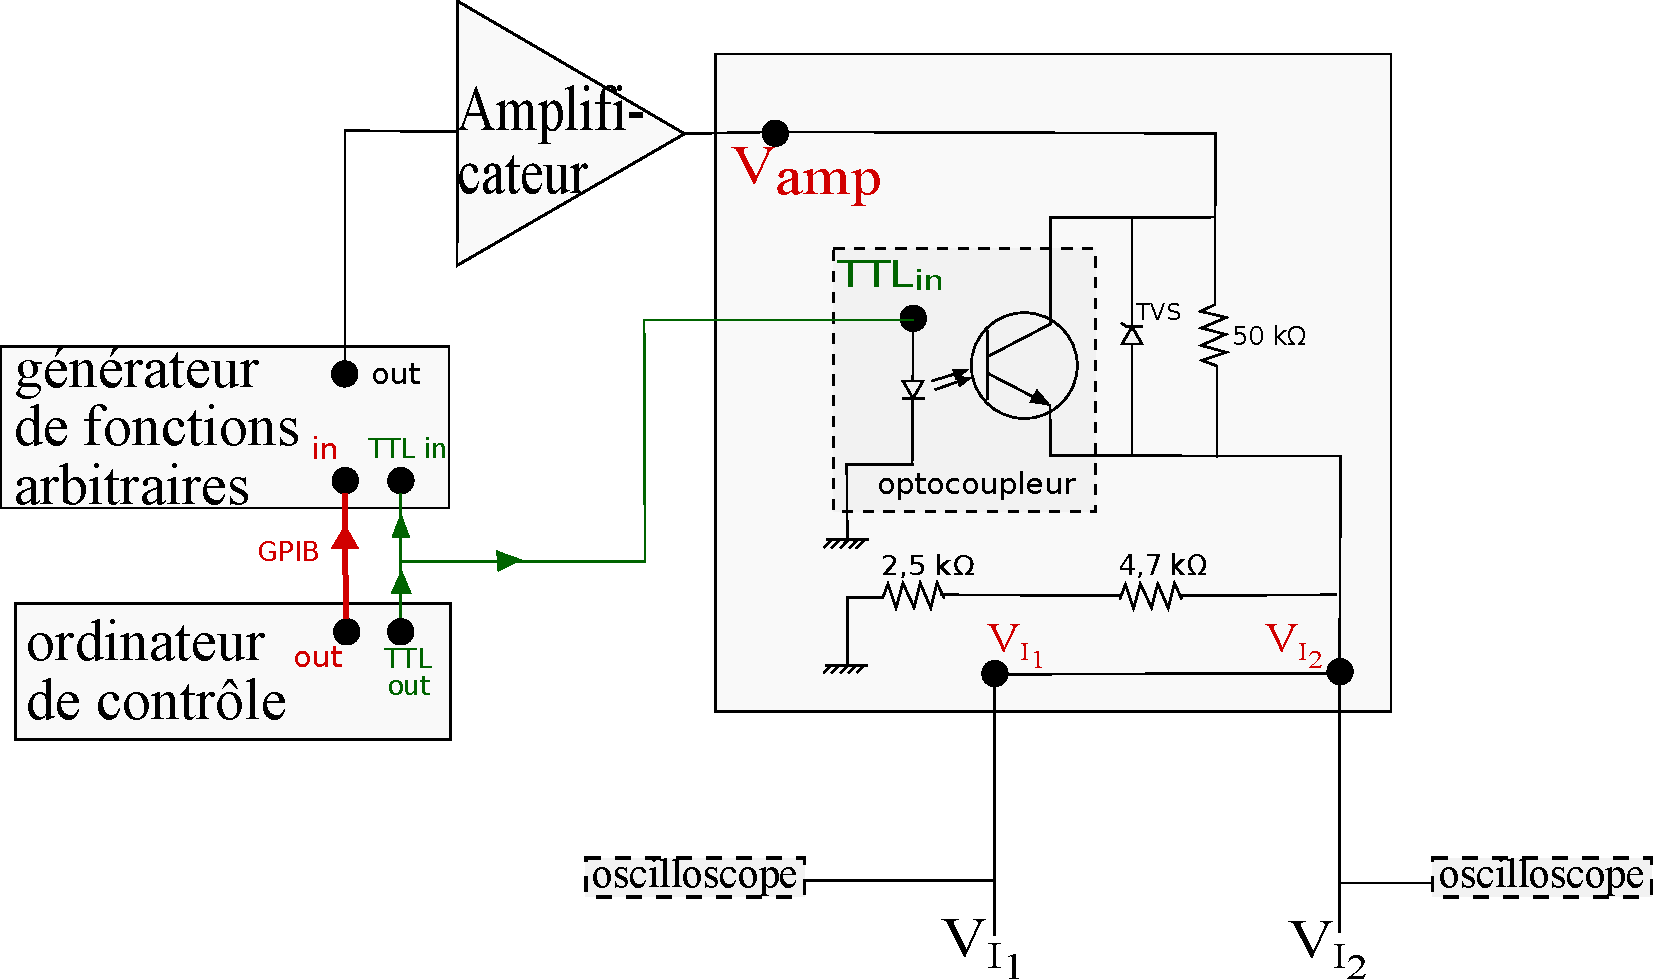
\includegraphics[width=.8\linewidth]{figures/setup/rydberg/detectionbox_ENS}
\caption[Premier circuit de contrôle de la tension des électrodes d'ionisation]{
Premier circuit de contrôle de la tension des électrodes d'ionisation.
Les tensions sont fournies par un générateur de fonctions arbitraires contrôlé par ordinateur, puis amplifiées par un amplificateur haute tension de gain $\times \num{50}$, délvrant jusqu'à $\pm \SI{150}{\V}$.
Pendant l'excitation des atomes de Rydberg, l'optocoupleur est bloquant.
Le pont diviseur de tension créé par la résistance de $\SI{50}{\kilo\ohm}$ d'une part et de $\SI{2.5}{} + \SI{4.7}{\kilo\ohm}$ divise par un facteur $\num{8}$ le bruit électronique au niveau des électrodes, au prix d'une réduction d'autant du signal.
Pendant la phase de détection, l'optocoupleur est passant et le pont diviseur est ainsi court-circuité.
La tension appliquée aux électrodes est alors directement la tension en sortie de l'amplificateur.
}
\label{fig:detectionbox_ENS}
\end{figure}
%

%\clearpage
\subsection{Manipulation cohérente des états de Rydberg}\label{subsec:mw_spectro}

\noindent Nous avons jusqu'ici limité notre exposé à l'excitation laser d'atomes vers un niveau de Rydberg déterminé.
Or nos expériences reposent sur la manipulation des atomes de Rydberg entre plusieurs états, en vue de deux objectifs.
Le premier est la caractérisation des interactions entre niveaux de Rydberg et le second est le développement d'un système quantique pouvant servir de plateforme pour la simulation quantique.

Les différences d'énergie entre niveaux de Rydberg voisins, comme nous l'avons évoqué au chapitre \ref{chapter:Rydberg}, sont dans le domaine des microondes millimétriques.
Cela correspond grossièrement à des fréquences de transition de l'ordre de $\SI{10}{}$ à $\SI{100}{\GHz}$.
La spectroscopie de ces transitions (\og spectroscopie microonde \fg{}) est l'outil majeur dont nous disposons pour caractériser les atomes de Rydberg au-delà de la spectroscopie laser de la transition depuis le niveau fondamental.
Son application pour l'étude du mouvement d'un nuage dense d'atomes de Rydberg sera discutée à la fin du chapitre \ref{chapter:60s}.
Son application à l'étude des atomes de Rydberg circulaires et à leur manipulation cohérente sera discutée aux chapitres \ref{chapter:circsim} et \ref{chapter:50c}.

Ici, nous évoquerons la manipulation cohérente d'un \og qubit de Rydberg \fg{} réalisé entre les états $\mathrm{60S}$ et $\mathrm{61S}$, ainsi que l'utilisation de la spectroscopie de la transition $\mathrm{60S} \rightarrow \mathrm{60P}$ pour mesurer les champs électriques résiduels.
Ces deux expériences 
%ont été menées avant l'installation des électrodes RF, et avec le premier circuit de contrôle du champ électrique (cf. \ref{subsec:compensation}). Elles 
sont décrites en détail dans la thèse de Carla Hermann Avigliano \cite{PHD_HERMANN}.

%\clearpage
\subsubsection*{Un qubit de Rydberg d'une grande longévité}
\noindent Au sein de notre dispositif, la cohérence d'un système quantique à deux niveaux réalisé entre deux niveaux de Rydberg est limitée en premier lieu par l'inhomogénéité du champ électrique résiduel.
De bons candidats à la réalisation d'un tel qubit seront donc des niveaux dont la sensibilité au champ sera la plus faible possible ou, à défaut, la plus similaire possible.
Les coefficients d'effet Stark quadratique synthétisés en table \eqref{tab:Stark_60S} nous éclairent dans notre choix : nous utiliserons les niveaux $\mathrm{60S_{1/2}}$ et $\mathrm{61S_{1/2}}$.
La quantité pertinente ici est le décalage en fréquence de la transition par l'effet Stark différentiel entre ces deux niveaux.
Celui-ci vaut $A_{\mathrm{60S1/2,61S1/2}} = \SI{-11}{\MHz \per (\V \per\cm) \squared}$.
La spectroscopie de la transition $\ket{g}=\ket{\mathrm{60S_{1/2},m_j=1/2}} \rightarrow \ket{e}=\ket{\mathrm{61S_{1/2},m_j=1/2}}$ est présentée en figure \eqref{fig:spectro_60S61S}.

La largeur de raie de $\Delta\nu=\SI{6.6}{\kHz}$ est de bon augure pour la manipulation cohérente de ce qubit.
Afin d'estimer son temps de cohérence de façon plus précise, nous avons effectué une spectroscopie Ramsey avec écho de spin entre les deux niveaux, dont le principe est schématisé en figure \eqref{fig:spinEcho_60S61S}.

\begin{figure}[h]
\centering
\vspace{1em}
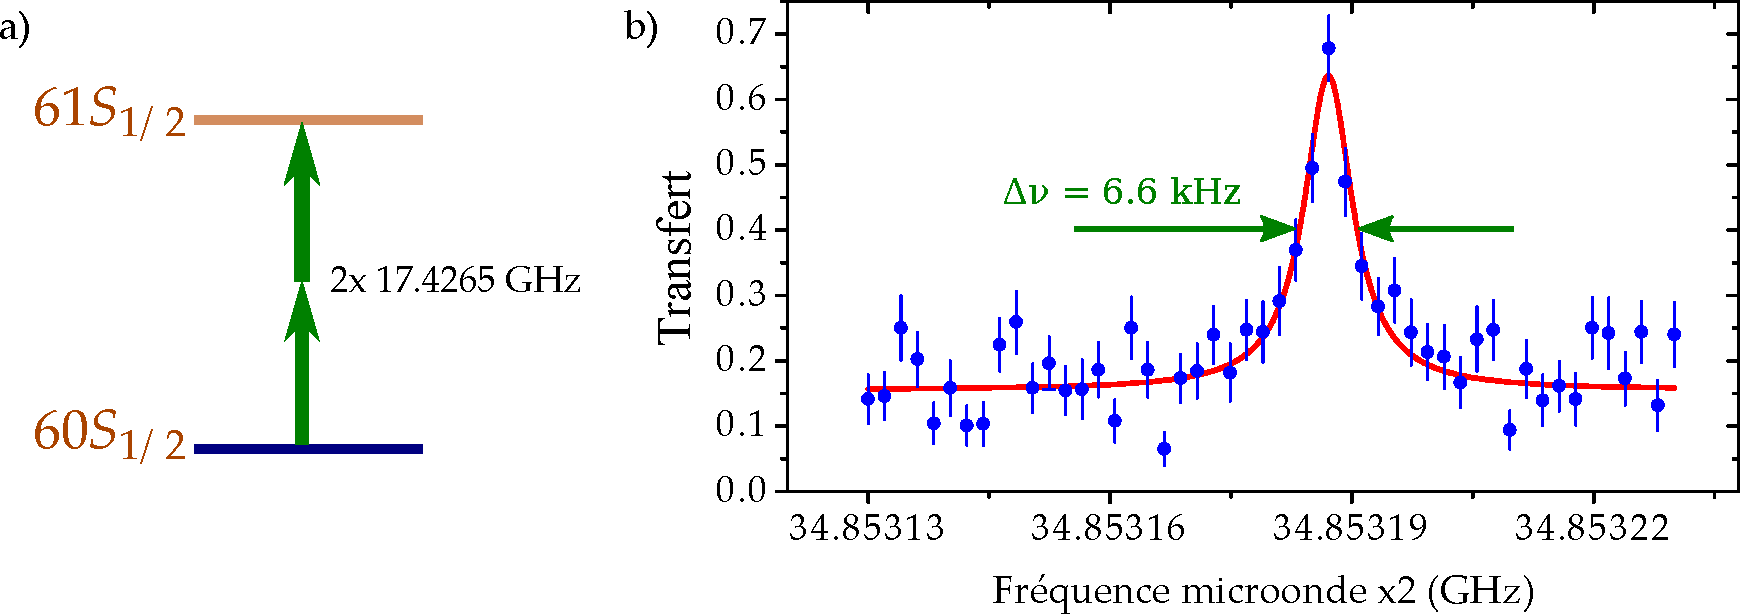
\includegraphics[width=.8\linewidth]{figures/setup/rydberg/spectro_60S61S}
\caption[Spectroscopie de la transition 60S-61S]{
Spectroscopie de la transition 60S-61S.
\textbf{a)} Diagramme de niveaux de la transition microonde à deux photons.
\textbf{b)} Spectre micro-onde de la transition, pour une durée d'excitation de $\SI{300}{\us}$. La courbe rouge est un ajustement lorentzien.
}
\label{fig:spectro_60S61S}
\end{figure}

\begin{figure}[!h]
\centering
\vspace{1em}
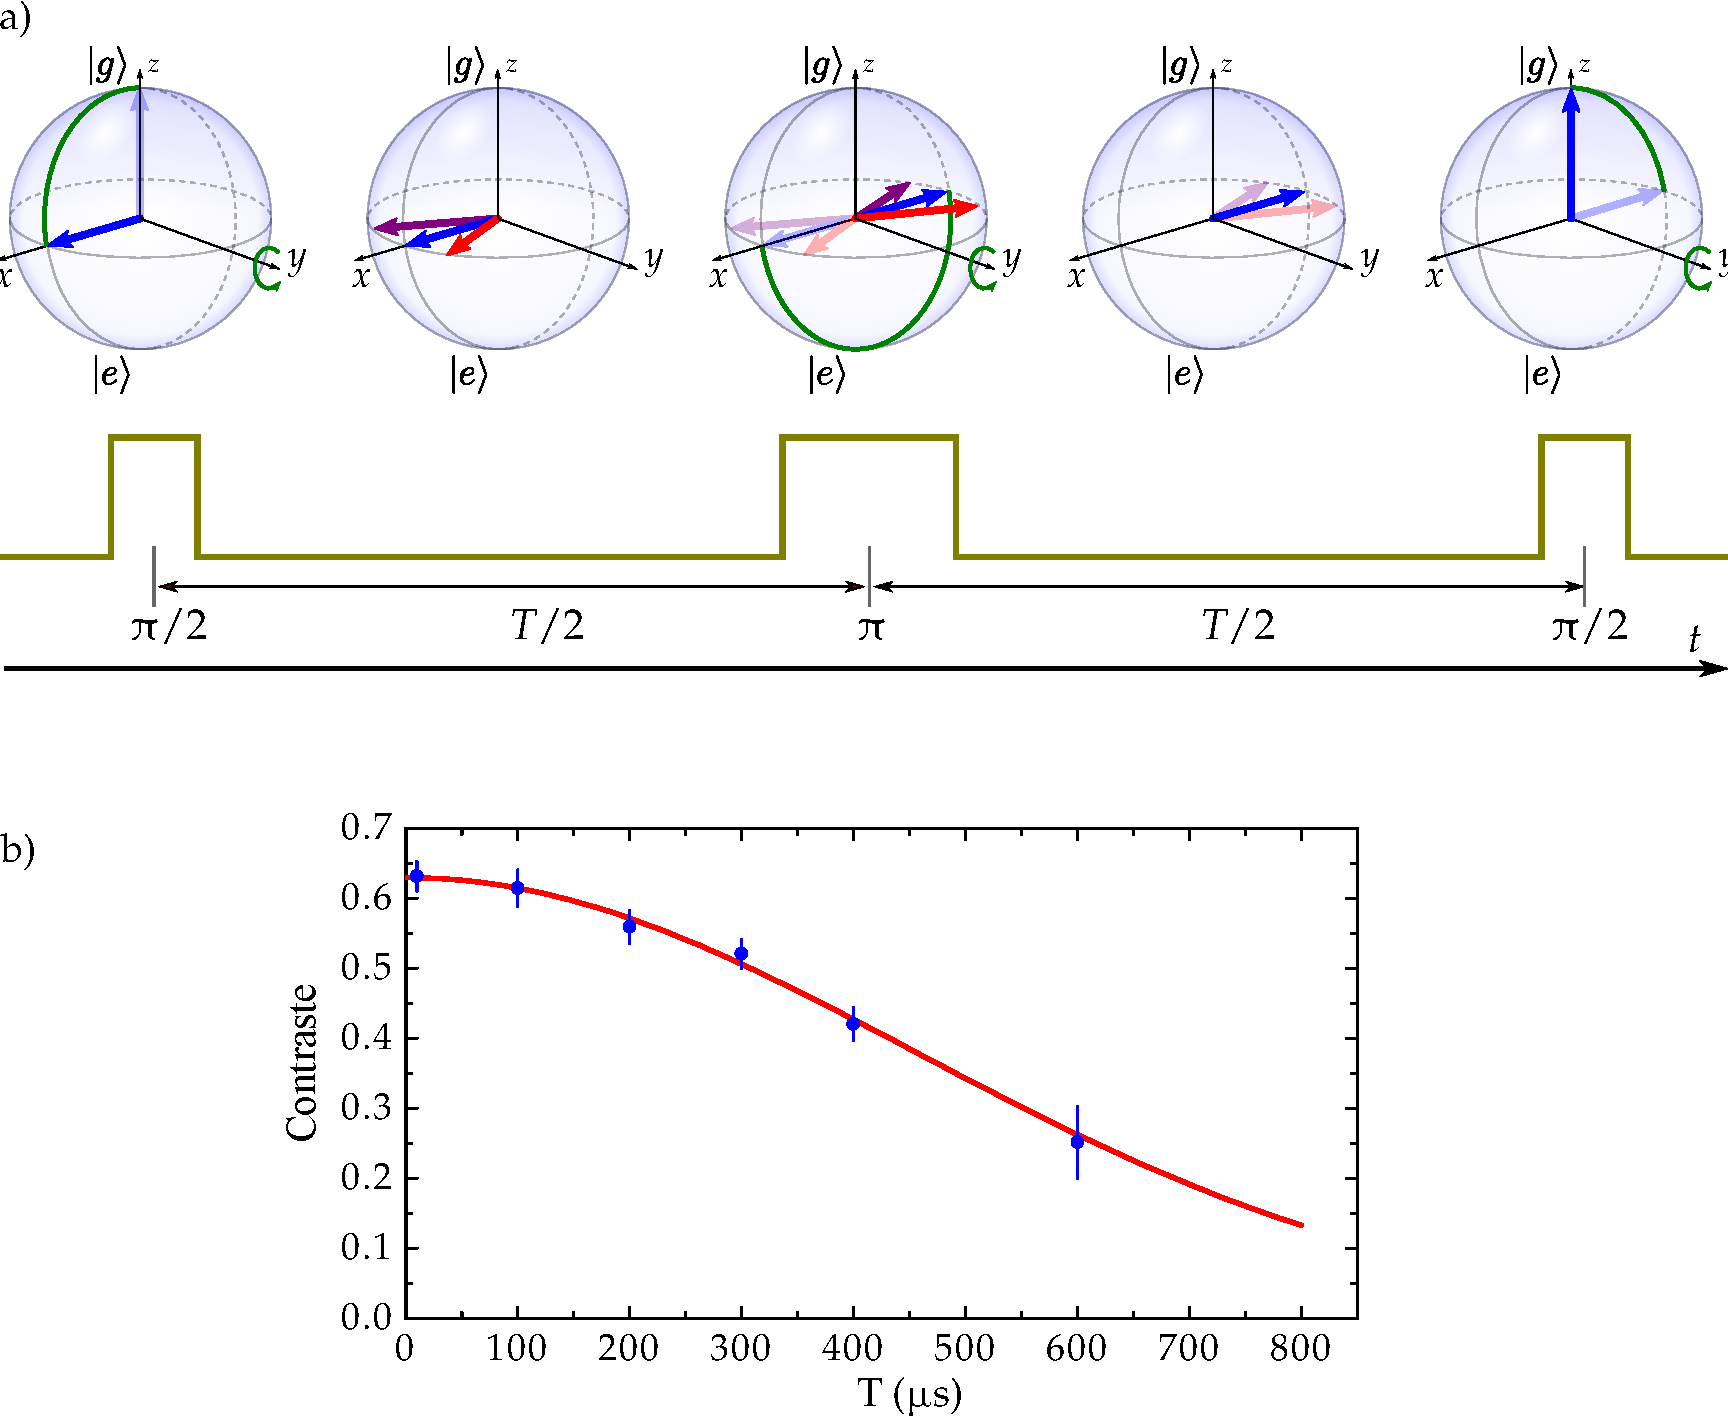
\includegraphics[width=.8\linewidth]{figures/setup/rydberg/spinEcho_60S61S}
\caption[Écho de spin 60S-61S]{
Spectroscopie Ramsey avec écho de spin sur la transition 60S-61S.
\textbf{a)} Principe de l'écho de spin représenté sur la sphère de Bloch. $\ket{g}$ et $\ket{e}$ représentent les états $\mathrm{60S_{1/2}}$ et $\mathrm{61S_{1/2}}$ respectivement.
\textbf{b)} Contraste des franges de Ramsey avec écho de spin, en fonction de la durée de $T$ de l'intervalle d'évolution. La courbe rouge est un ajustement gaussien.
}
\label{fig:spinEcho_60S61S}
\end{figure}

\newpage
La technique d'écho de spin permet de se libérer des sources de décohérence stables dans le temps, telles que l'inhomogénéité spatiale du champ électrique.
L'impulsion $\pi$ intercalée à la moitié de l'évolution de la superposition d'état agit comme un renversement du temps.
Les effets de déphasage de la superposition ne variant pas dans le temps sont ainsi compensés dans la deuxième moitié de son évolution.
L'ajustement gaussien du contraste des franges de Ramsey en fonction du temps total d'évolution permet d'extraire un temps de cohérence à $1/e$ de la superposition de $T_2 = \SI{631}{\us}$.
Ce temps de cohérence est trois fois supérieur à la durée de vie des niveaux de Rydberg, qui est de l'ordre de $\SI{200}{\us}$.
Cela signifie que, alors que la plupart des atomes de Rydberg ont été perdus par désexcitation radiative, ceux qui ne l'ont pas été, donc ceux que nous détectons, gardent leur cohérence pendant une durée $T_2$.

%\clearpage
\subsubsection*{Mesure des champs électriques résiduels}
\noindent La même technique de spectroscopie microonde nous a permis de mesurer les champs électriques résiduels.
Pour cela, à l'inverse de l'expérience précédente, nous voulions une transition aussi sensible que possible à l'effet Stark.
Nous avons donc choisi la transition $\mathrm{60S}\rightarrow\mathrm{60P}$., qui présente un effet Stark quadratique de .
Celle-ci se sépare par effet Zeeman entre les transitions $\mathrm{60S_{1/2},m_j=1/2} \rightarrow \mathrm{60P_{3/2},m_j=-1/2}$ %, présentant un effet Stark différentiel de $\SI{586.1}{\MHz \per (\V \per\cm) \squared}$ 
et $\mathrm{60S_{1/2},m_j=1/2} \rightarrow \mathrm{60P_{3/2},m_j=+3/2}$, qui présentent des effets Stark différentiels de $\SI{586.1}{}$ et $\SI{479.1}{\MHz \per (\V \per\cm) \squared}$ respectivement.
%Les atomes étant piégés dans le piège magnétique, l'effet Zeeman est ici important.
%En particulier, c'est le champ magnétique qui détermine l'axe de quantification, et donc l'axe de symétrie de la fonction d'onde des niveaux $P$.
%Pour cette raison, un champ électrique parallèle au champ magnétique produira un déplacement d'énergie par effet Stark différent d'un champ électrique perpendiculaire au champ magnétique.
L'anistropie des niveaux $P$ en présence d'un champ magnétique, ici celui qui sert à piéger les atomes, nous a permis d'estimer indépendamment le champ électrique résiduel perpendiculairement et parallèlement à la puce.
Le champ résiduel perpendiculaire à la puce a été mesuré à $\SI{0.09}{\V/cm}$, cette valeur pouvant être compensée par l'application d'une tension sur les électrodes d'ionisation.
Le champ parallèle à la puce a été mesuré à $\SI{0.09}{\V/cm}$ à $\SI{150}{\um}$ de la puce, décroissant jusqu'à des valeur comprise entre $\SI{0.05}{}$ et $\SI{0.06}{\V/\cm}$ pour des distances à la puce supérieures à $\SI{300}{\um}$.
Ce champ résiduel parallèle à la puce ne pourra être compensé qu'après installation des électrodes RF.

Enfin, cette expérience nous a permis d'estimer les gradients résiduels du champ électrique au voisinage de la puce, à partir de la taille du nuage et de la largeur des raies spectrales de transition, principalement due à un élargissement Stark inhomogène, tel que présenté en \ref{subsec:flashRb}.
Ces estimations ont été faites dans l'approximation d'un gradient de champ constant et principalement situé sur la composante $F_x$.
La table \ref{tab:fieldGrad} synthétise ces mesures.
%
\begin{table}[!h]
	\centering
	\caption[Estimation des gradients de champ électrique près de la puce]{Gradient de champ électrique au voisinage de la puce, à différentes distances.%, selon les directions $x$ et $z$.
	}
	\label{tab:fieldGrad}
	\begin{tabular}{c c c}
		\toprule\midrule
		Distance à la puce
		& $\partial |F| / \partial x$
		& $\partial |F| / \partial z$\\		
		$\si{\um}$
		& $\si{(\V/\cm)\squared}$
		& $\si{(\V/\cm)\squared}$\\
		\midrule
		\SI{150}{} & \SI{1.428}{} & \SI{21.714}{} \\
		\SI{245}{} & \SI{1.504}{} & \SI{9.023}{} \\
		\SI{338}{} & \SI{2.166}{} & \SI{11.597}{} \\
		\SI{455}{} & \SI{1.566}{} & \SI{9.011}{} \\
		\SI{555}{} & \SI{0.9}{} & \SI{5.088}{} \\
		\SI{675}{} & \SI{0.76}{} & \SI{4.277}{} \\
		\midrule
		\bottomrule
 	\end{tabular}
\end{table}
%

Nous pouvons en déduire que la distance à la puce à laquelle nous choisissons de placer les atomes de Rydberg aura une influence déterminante sur leur exposition à un effet Stark inhomogène.

\subsection{Temps de vie des atomes de Rydberg et température effective}\label{subsec:lifetime}
\noindent Nous avons calculé, au chapitre \ref{chapter:Rydberg}, la durée de vie du niveau $\mathrm{60S}$ à différentes températures.
La figure \ref{fig:lifetime_60S} montre une mesure expérimentale du nombre d'atomes de Rydberg détectés dans le nuage atomique, en fonction du délai entre l'excitation et la détection des atomes de Rydberg.

L'ajustement exponentiel de cette mesure donne un temps de vie de $\tau_{\mathrm{60S}} = \SI{210}{} \pm \SI{4}{\us}$, alors que le temps de vie théorique calculé à la température de l'hélium liquide vaut $\SI{239.8}{\us}$ (cf table \ref{tab:lifetime_60S}).
La différence de temps de vie peut s'expliquer par différents effets :
les atomes sont exposés au rayonnement du corps noir à température ambiante et à la température de l'azote liquide, qui peut entrer par les hublots d'accès optique.
De plus, la géométrie complexe des surfaces conductrices au voisinage des atomes (puce et électrodes) changent la densité de mode du rayonnement électromagnétique par rapport à celle du vide.

Afin de rendre compte simplement de ces effets, nous calculons une température effective.
C'est la température pour laquelle le calcul du temps de vie théorique présenté au chapitre \ref{chapter:Rydberg} donnerait la valeur de temps de vie mesurée.
Cette température effective pour le niveau $\mathrm{60S}$ dans notre cryostat est de $\SI{36}{\kelvin}$.

\begin{figure}[h]
\centering
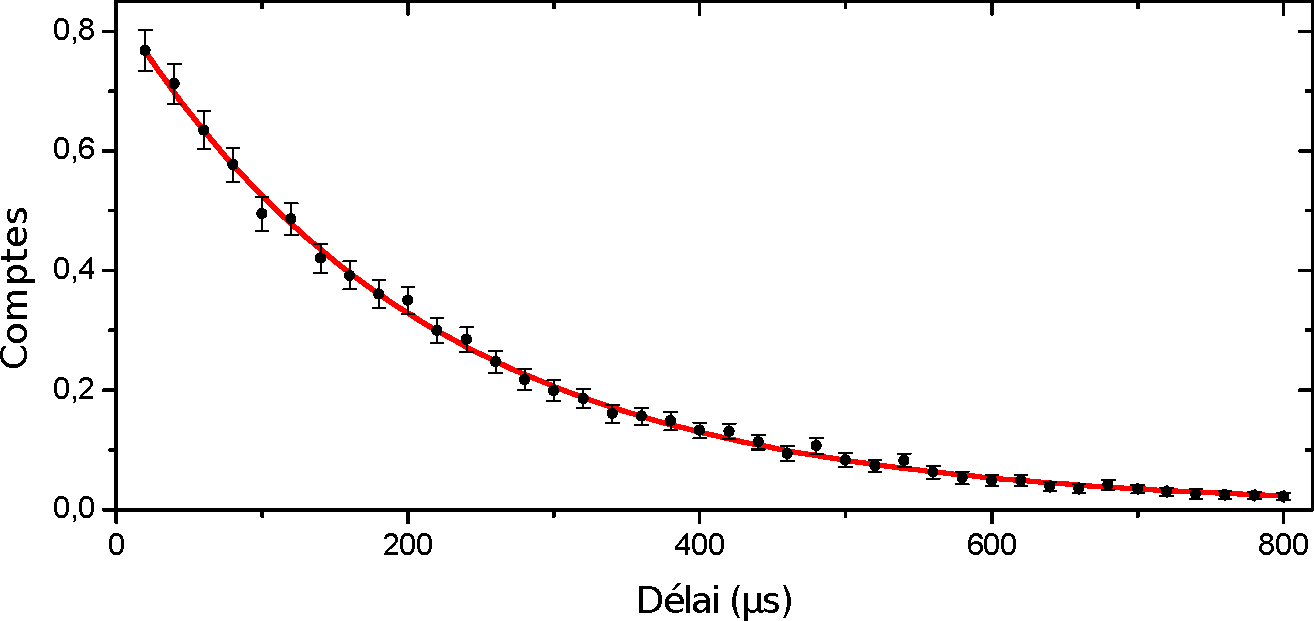
\includegraphics[width=0.8\linewidth]{figures/setup/rydberg/lifetime_60S}
\caption[Durée de vie du niveau 60S]{
Nombre d'atomes de Rydberg dans le niveau $\mathrm{60S}$ détectés, en fonction du délai entre l'impulsion laser d'excitation et la rampe d'ionisation servant à leur détection.
L'ajustement exponentielle donne un temps de vie de $\SI{210}{} \pm \SI{4}{\us}$.
}
\label{fig:lifetime_60S}
\end{figure}

\section*{Conclusion}
\noindent Nous avons, dans le présent chapitre, décrit le fonctionnement du dispositif expérimental sur lequel nous avons effectué nos travaux.
Le dispositif cryogénique et la puce à atomes nous permettent de piéger et refroidir des nuages d'atomes de \Rb{87} jusqu'à la condensation de Bose-Einstein.
Un second aspect du dispositif nous permet d'exciter, manipuler et détecter des atomes de Rydberg au sein de ces nuages d'atomes ultra-froids.

La difficulté particulière que présente la manipulation d'atomes de Rydberg près d'une surface, due à leur très grande sensibilité au champ électromagnétique, a été surmontée par le dépôt contrôlé d'une couche macroscopique de rubidium sur la surface de la puce atomique.
Ce dépôt garantit en effet une bonne homogénéité des champs électriques résiduels, mise en évidence par l'étroitesse des raies de transition optique et par la longévité du qubit de Rydberg réalisé entre les niveaux $\mathrm{60S}$ et $\mathrm{61S}$.

Nous disposons ainsi 
%, malgré ses fortes exigences techniques,
d'un dispositif performant et prometteur pour l'étude des interactions entre atomes de Rydberg.
% froids.